% !TEX encoding = UTF-8 Unicode
% !TEX root = DesignDocument.tex

\documentclass{book}

% !TEX root = SystemTemplate.tex

\usepackage[width=6.5in, height=9.2in, top=1.0in, papersize={8.5in,11in}]{geometry}
\usepackage[pdftex]{graphicx}
%\usepackage{draftwatermark}
\usepackage{amsmath}
\usepackage{amsthm}
\usepackage{amssymb}
%\usepackage{txfonts}
\usepackage{textcomp}
%\usepackage{amsthm}

\usepackage[all]{xy}
\usepackage{fancyhdr}
\pagestyle{fancy}
\usepackage{hyperref}
\usepackage{verbatim}
\usepackage{algorithm}
\usepackage{algorithmic}
\usepackage{array}
\usepackage{color}
\usepackage{listings}
\lstset{language=c,frame=ltrb,framesep=5pt,basicstyle=\normalsize,
 keywordstyle=\ttfamily\color{DarkRed},
identifierstyle=\ttfamily\color{DarkBlue}\bfseries,
commentstyle=\color{OliveGreen},
stringstyle=\ttfamily,
showstringspaces=false,tabsize = 3}
\usepackage{calc}
\usepackage{doxygen}
\usepackage[utf8]{inputenc}
\usepackage{makeidx}
\usepackage{multicol}
\usepackage{multirow}
\usepackage[table]{xcolor}
\usepackage{tabularx}
\usepackage{framed}
\usepackage{xspace}
\usepackage{etex}
\usepackage{todonotes}
\usepackage{pdfpages}
\usepackage{pgfgantt}


\definecolor{color02}{rgb}{0.18,0.35,0.59}
\definecolor{color03}{rgb}{0.44,0.59,0.82}
\definecolor{color06}{rgb}{0.35,0.35,0.35}


\newtheorem{summary}{Summary:}
\newtheorem{example}{Example:}


\definecolor{OliveGreen}{cmyk}{0.64,0,0.95,0.40}
\definecolor{DarkBlue}{cmyk}{0.76,0.76,0,0.20}
\definecolor{DarkRed}{cmyk}{0,1,1,0.45}


\def      \RR             {{\mathbb R}} 
\def      \DS            {\displaystyle} 

\setlength{\oddsidemargin}{0mm} 
\setlength{\evensidemargin}{0mm} 

%\SetWatermarkLightness{0.975}
%\SetWatermarkScale{6}
%\SetWatermarkText{\includegraphics{test.png}}

\pagestyle{fancy}
\renewcommand{\chaptermark}[1]{\markboth{#1}{}}
\renewcommand{\sectionmark}[1]{\markright{\thesection\ #1}}
\fancyhf{}
\fancyhead[LE,RO]{\bfseries\thepage}
\fancyhead[LO]{\bfseries\rightmark}
\fancyhead[RE]{\bfseries\leftmark}
%\fancyfoot[LE,RO]{Confidential and Proprietary}
%\renewcommand{\headrulewidth}{0.5pt}
%\renewcommand{\footrulewidth}{0pt}
%\addtolength{\headheight}{0.5pt}
%\setlength{\footskip}{0mm}
%\renewcommand{\footruleskip}{0pt}


\definecolor{MSBlue}{rgb}{.204,.353,.541}
\definecolor{MSLightBlue}{rgb}{.31,.506,.741}
\definecolor{MSBlue1}{rgb}{0.18,0.35,0.59}
\definecolor{MSBlue2}{rgb}{0.44,0.59,0.82}
\definecolor{MSBlue3}{rgb}{0.35,0.35,0.35}


\usepackage{titlesec}
\titleformat{\chapter}[display]
{\normalfont\bfseries\color{MSBlue1}}    %\normalfont\bfseries\filcenter}
{\LARGE\thechapter}
{1ex}
{\titlerule[2pt]
\vspace{2ex}%
\LARGE}
[\vspace{1ex}%
{\titlerule[2pt]}]

\definecolor{MSBlue}{rgb}{.204,.353,.541}
\definecolor{MSLightBlue}{rgb}{.31,.506,.741}
\definecolor{MSBlue1}{rgb}{0.18,0.35,0.59}
\definecolor{MSBlue2}{rgb}{0.44,0.59,0.82}
\definecolor{MSBlue3}{rgb}{0.35,0.35,0.35}

%\titleformat*{\section}{\Large\bfseries\sffamily\color{MSBlue}}
%\titleformat*{\subsection}{\large\bfseries\sffamily\color{MSLightBlue}}
%\titleformat*{\section}{\Large\bfseries\color{MSBlue1}}
%\titleformat*{\subsection}{\large\bfseries\color{MSBlue2}}

\titleformat*{\section}{\Large\bfseries\color{MSBlue}}
\titleformat*{\subsection}{\large\bfseries\color{MSLightBlue}}
\titleformat*{\subsubsection}{\large\bfseries\color{MSBlue3}}
\setcounter{secnumdepth}{3}
\renewcommand{\thesubsubsection}{\thesubsection.\alph{subsubsection}}

% Save the original chapter command as stdchapter
\let\stdchapter\chapter

%redefine the backmatter command
\let\stdbackmatter\backmatter
\makeatletter% We need the '@' letter to call if@openright
\renewcommand{\backmatter}{
\stdbackmatter
% need to set the page counter back to 1
\setcounter{page}{1}
%% Redefine the \chapter command for our Back Matter
\renewcommand{\chapter}[1]{
  \if@openright\cleardoublepage\else\clearpage\fi% chapters begin on right page
  \stdchapter{##1}% output standard chapter heading
  \setcounter{section}{0}% restart the section numbering
  \renewcommand{\thepage}{BM-\arabic{page}}% Redefine page numbering format
  \renewcommand{\thesection}{\arabic{section}}% Redefine section number format
}}
\makeatother% Restore the normal behavior of '@'

%redefine the appendix command
\let\stdappendix\appendix
\makeatletter% We need the '@' letter to call if@openright
\renewcommand{\appendix}{
\stdappendix
%% \titleformat{\chapter}[display]
%% {\normalfont\bfseries\color{MSBlue1}}    %\normalfont\bfseries\filcenter}
%% {\LARGE Appendix \thechapter}
%% {1ex}
%% {\titlerule[2pt]
%% \vspace{2ex}%
%% \LARGE}
%% [\vspace{1ex}%
%% {\titlerule[2pt]}]
  %%% Since counters are different in the appendix section
  %%% we redefine \chapter to explicitly reset the page number
  %%%  (comment out to see effect)
  \renewcommand{\chapter}[1]{
    \stdchapter{##1}\setcounter{page}{1}
    %%% We also redefine page numbering
    \renewcommand{\thepage}{\Alph{chapter}-\arabic{page}}
  }
}
\makeatother% Restore the normal behavior of '@'


\makeatletter% We need the '@' letter to call if@openright
\newcommand{\agreement}{
  \renewcommand{\chapter}[1]{
    \if@openright\cleardoublepage\else\clearpage\fi% chapters begin on right page
    \pagestyle{plain}% turn off fancy headers
    \setcounter{section}{0}% Reset the section number
    \setcounter{page}{1}% Reset the page number
    \renewcommand{\thepage}{SA-\arabic{page}}% Set format for page numbering
    \renewcommand{\thesection}{\arabic{section}}% Set format for section numbering
    \refstepcounter{chapter}% Add it to the index/toc for on-line viewing
    \addcontentsline{toc}{chapter}{##1}% Add to the table of contents
  }
}
\makeatother% Restore the normal behavior of '@'


 % This sets the format.

% Add your title page contents here 
\title{{\color{SDColor3} \rule{\linewidth}{0.5mm}}\\[2mm] {\huge \bfseries \color{SDColor3} Crowd Control }\\[-1mm] {\color{SDColor3}\rule{\linewidth}{0.5mm}} \\  \vfill
{\LARGE \bfseries \color{SDColor4} Senior Design Final Documentation }\\  \vfill 
{\color{SDColor3} Bowtaps} }
\author{\color{SDColor3}  Johnathan Ackerman \and \color{SDColor3} Daniel Andrus\and  \color{SDColor3} Charles Bonn \and \color{SDColor3} Evan Hammer\and \color{SDColor3} Joseph Mowry }
\date{\color{SDColor3} \today}


\begin{document}

\frontmatter

\addcontentsline{toc}{chapter}{Title}
\maketitle
\tableofcontents
\addcontentsline{toc}{chapter}{Contents}
\listoffigures
\addcontentsline{toc}{chapter}{List of Figures}
\listoftables
\addcontentsline{toc}{chapter}{List of Tables}
\listofalgorithms
\addcontentsline{toc}{chapter}{List of Algorithms}\

\chapter{Overview Statements}
% !TEX root = DesignDocument.tex

\section{Mission Statement}
Mission statement inserted here.   

\section{Elevator Pitch}
Elevator Pitch inserted here.   
  % add mission statement to mission.tex

\chapter{Document Preparation and Updates}
% !TEX root = DesignDocument.tex



Current Version [1.5.3]
\vspace*{5mm}

{\color{SDColor5}
\noindent
\textit{Prepared By:}\\
\textit{Johnathan Ackerman}\\
\textit{Daniel Andrus}\\
\textit{Charles Bonn}\\
\textit{Evan Hammer}\\
\textit{Joseph Mowry}
}
\vfill
\noindent
{\color{SDColor3} \textit{\textbf{Revision History}}}\\
\begin{tabular}{|>{\raggedright}p{1.5cm}|>{\raggedright}p{3cm}|>{\raggedright}p{1.5cm}|>{\raggedright}p{9cm}|}
\hline
\textit{\textbf{Date}} &  \textit{\textbf{Author}} & \textit{\textbf{Version}} & \textit{\textbf{Comments}}\tabularnewline
\hline
 \textit{\textbf{10/1/15}} & \textit{Charles Bonn} & \textit{1.0.0} & \textit{Sprint 1 \& Senior Design Contract}\tabularnewline
 \hline
  \textit{\textbf{11/3/15}} & \textit{Charles Bonn} & \textit{1.1.0} & \textit{Sprint 2 Documentation}\tabularnewline
 \hline
 \textit{\textbf{12/11/15}} & \textit{Charles Bonn} & \textit{1.2.0} & \textit{Sprint 3 finished, résumés added}\tabularnewline
\hline
 \textit{\textbf{1/15/16}} & \textit{Daniel Andrus} & \textit{1.2.1} & \textit{iOS documentation added}\tabularnewline
\hline
 \textit{\textbf{1/18/16}} & \textit{Joseph Mowry} & \textit{1.3.0} & \textit{Winter Sprint Report added}\tabularnewline
\hline
 \textit{\textbf{2/12/16}} & \textit{Charles Bonn} & \textit{1.4.0} & \textit{Sprint 4 Report, general content added}\tabularnewline
\hline
 \textit{\textbf{2/18/16}} & \textit{Joseph Mowry} & \textit{1.5.0} & \textit{Sprint 5 Report, various chapter revisions}\tabularnewline
\hline
 \textit{\textbf{2/19/16}} & \textit{Charles Bonn} & \textit{1.5.1} & \textit{Sprint 5 Report, organizational changes, chapter revisions}\tabularnewline
\hline
 \textit{\textbf{2/24/16}} & \textit{Johnathan Ackerman} & \textit{1.5.2} & \textit{Overview rewrite}\tabularnewline
\hline
 \textit{\textbf{3/17/16}} & \textit{Evan Hammer} & \textit{1.5.3} & \textit{Document cleanup, organizational changes}\tabularnewline
\hline
\textit{\textbf{4/29/16}} & \textit{Johnathan Ackerman} & \textit{1.6.0} & \textit{Completed Chapter 6}\tabularnewline
\hline
\textit{\textbf{4/22/16}} & \textit{Joeseph Mowry} & \textit{1.6.1} & \textit{Completed Chapters 0, 1}\tabularnewline
\hline
\textit{\textbf{4/30/16}} & \textit{Evan Hammer} & \textit{1.6.2} & \textit{Completed Chapters 2, 3}\tabularnewline
\hline
\textit{\textbf{5/2/2016}} & \textit{Joeseph Mowry} & \textit{1.6.3} & \textit{Completed Chapter 4}\tabularnewline
\hline
\textit{\textbf{5/2/2016}} & \textit{Charles Bonn} & \textit{1.6.4} & \textit{Completed Chapters 8, 9, 10}\tabularnewline
\hline
\textit{\textbf{5/2/2016}} & \textit{Johnathan Ackerman} & \textit{1.6.5} & \textit{Completed Chapter 7}\tabularnewline
\hline
\textit{\textbf{5/3/2016}} & \textit{Dan Andrus} & \textit{1.6.6} & \textit{Completed Chapter 5}\tabularnewline
 &  &  & \tabularnewline
\hline
\end{tabular}
\vfill


 
\mainmatter

%% The term "cleaning" used in the syllabus means removing all of the sample content I
%% have provided.   You can comment out by using the comment character or the comment
%% environment.  

%%  Add to the following chapters

% !TEX root = DesignDocument.tex


\chapter{Overview and Concept of Operations}

%The overview should take the form of an executive summary.  Give the reader a feel 
%for the purpose of the document, what is contained in the document, and an idea 
%of the purpose for the system or product. 

\section{Bowtaps and Its Team}

Bowtaps is a start up company from Rapid City, SD that began working together at the SDSM\&T campus. Our goal is to create easy to use software applications that help ease the everyday life of the user. Their software aims to be both well-constructed and maintainable, and their products are made with sustainability in mind. Bowtaps currently consists of the members Charles Bonn, Johnathan Ackerman, Daniel Andrus, Evan Hammer, and Joesph Mowry. Their roles and experience are further detailed in section C of this document.

\section{Crowd Control}
Crowd Control is our flagship product designed and created by Bowtaps. Its goal is to combine GPS tracking, group messaging and group management features into one easy to use application. A primary focus of this product is to be maintainable and modular, so that if better solutions arise, those can be implemented with minimal refactoring.

User information is perhaps our greatest focus in Crowd Control's design; careful measures were taken to assure that sensitive user information is kept safely, vulnerabilities are removed, and risks are mitigated. Before Crowd Control is released to the public, we will implement an encryption scheme called AES-256. Bowtaps also uses third-party services such as Parse and Sinch that guarantee safety in storage and transmission of data through their access points.

Crowd Control, in addition to being written in a maintainable, well-designed manner, is aimed to be a sustainable commercial product. Bowtaps is using what they have gathered from various business accelerators and entrepreneurship-focused learning material to apply those concepts to the real-life startup company, Bowtaps, LLC. Bowtaps uses their recently acquired business skills to market Crowd Control, project associated finances, and seek investors for expansion.

\subsection{Purpose of the System}
Crowd Control is a mobile application designed to ease the experience of going out though the implementation of integrated group messaging, GPS tracking and group management features. Along with the features to manage your group at the event Crowd Control also gives suggestions of local events, restaurants and attraction. This allows the group to continue even when the next item on the agenda is a mystery. 

Even though Crowd Control is initially designed for the event-goer scene, it's uses can be expanded to fit more purposes. Crowd Control can be used to help manage any kind of group at an event such as church groups, tour groups, or school field trips.

\section{Business Need}
\begin{comment}
Use this section to define what business need exist and how this software will 
meet and/or exceed that business need.   (still fill out)
\end{comment}

Currently, there is no product on the market that encompasses all the features of group management, in-app messaging, and GPS tracking in one easy-to-use package. For example, Facebook is a popular option for group messaging and event creation, but it doesn't allow users to track each other for a duration of time. Crowd Control allows for both group messaging and event creation, as well as GPS tracking and better group management, specifically tailored to those at an event. Facebook's limited group management features are specifically designed for planning an event ahead-of-time, not necessarily managing during an event.

Crowd Control not only addresses the needs of those seeking group management/communication during events, but also helps serve as a platform for businesses to advertise themselves to users in the form of events and promotions. Those events are available in the form of nearby events that users can choose to set as their destination upon creating a group. This is a mutually beneficial feature for the users and for the businesses themselves.

\section{Deliverables}
\begin{comment}
Provide a complete description of the client requested deliverables.   This section should be the section your software contract references.   ( still fill out)
\end{comment}
The deliverables for this two-semester senior design project are the following items:
	\begin{itemize}
	  \item Crowd Control mobile application
	  \item Associated JavaDoc documentation
	  \item Senior Design document - some included items include:
	  	\begin{itemize}
		  \item General documentation
		  \item User manual and various code documentation
		  \item Business plan for Bowtaps, LLC
		  \item Sprint reports
		\end{itemize}
	  \item Design fair presentation
	\end{itemize}


\section{System Description}
Behind the UI, Crowd Control is written using an MVC architecture. IOS is written natively in Swift under the IDE XCode. On the Android side, the code is written in Native Mobile Java under Android Studio.

The code for Android uses XML files for storing layout-related code, which act as the view in the MVC pattern. Each activity acts as a controller. Each one of the models has an interface, which is how the controllers get access to the functions and data provided by the model. Each interface is set up in such a way that it uses OOP inheritance to generalize the models, thus abstracting our third party software. This contract allows us to write our code in such a way that, if ever needed, we could change the underlying implementation of certain modules with minimal refactoring.\\\\
%Remove explicit newlines after iOS section is taken care of.
The iOS platform follows a very similar MVC design pattern, too.\\
(TODO: iOS details needed.)

\subsection{Integrated Group Messaging}
Integrated group messaging is an important feature of Crowd Control. It allows for communication between cross platform, different phone brands, and different carriers. This allows for seamless communication between users with out the issues associated with messaging such as messages not using the same format, messages not going to all recipients, and messages with users in the group that you do not want to have your personal information.

Currently this is handled by a third party called Sinch. Sinch messaging handles the encryption of messages for the security of our users. Also, Sinch uses app to app messaging. In this way, any device with Crowd Control can send a message to other group members. However, since our app is currently only implemented on Android, messages can only be passed between Android users. It only needs either an internet connection or cell service to function.

\subsection{GPS Location services}
GPS allows for tracking of members in the group on a local map of the area. With this feature you will be able to keep track of anyone in the group off of their last GPS check in. This is useful to help locate members of the group that maybe lost or unable to be located. This feature will have the option of being able to opt out when the user does not want to have their location known to the group. When the users battery is low it will allow for the check in period to be extended or turned off to save battery life.


\subsection{Group Management Features}
The group management features allow for information to be shared with the group. A group management menu will allow for a group agenda to be posted as well as updates when the agenda changes. With the GPS features it will allow for the group leader to set way-points for the group.  

\subsection{Suggestions}
Suggestions are both a plus for the user and our way of making revenue. Suggestions are sponsored by local businesses in the form of an ad. Although these are not traditional ads, they are in the form of local points of interest such as restaurants, bars, amusement parks, or bowling allies. The possibilities are endless. With the suggestion method it will allow for our users to have helpful suggestions of places for their group to attend as well as exposure for the local businesses that are sponsoring Crowd Control.


\section{System Overview and Diagram}
The basic overview of Crowd Control can be seen in the diagram below. See Figure~\ref{ModuleFlowDiagram}. Crowd Control will be using a model-view-controller design structure. With the model view controller design method we are able to abstract the user interface from the control structures that will communicate with the third party services such as Parse, Google play services, or Sinch. The model of each respective operating system ( Android or iOS ) will be able to communicate with the respective mapping feature ( Google Play Services or Apple Map Features ). While both models will be able to communicate with Parse, our back end server. Though Parse, using their features, will be able to connect user profiles to their Facebook and twitter accounts for faster log in.

\begin{figure}[tbh]
\begin{center}
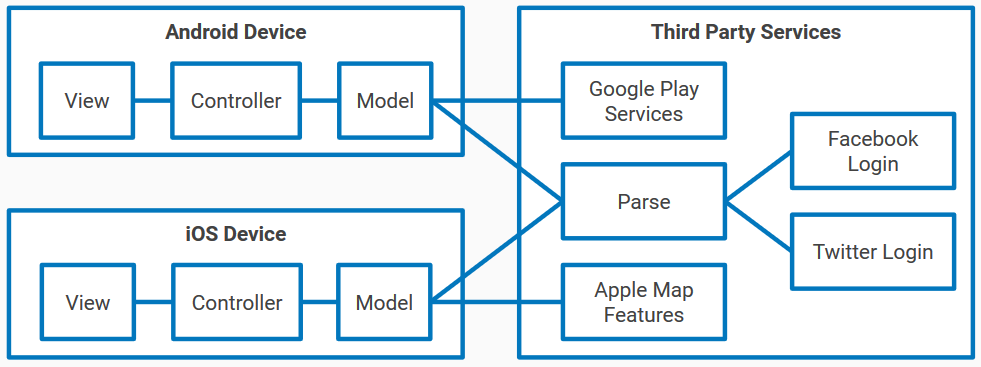
\includegraphics[width=0.75\textwidth]{Additional/designpictures/ModuleFlowDiagram.png}
\end{center}
\caption{Basic System Flow Diagram \label{ModuleFlowDiagram}}
\end{figure}

\section{Technologies Overview}
Some technologies used in the creation of Crowd Control are Google Play Services, Apple Map Features, Parse, Sinch, and Android Studio.

\subsection{Google Play Services}
	\subsubsection{Description}
	Google Play Services contains the native android API for mapping features. With this it allows for communication between a map and your GPS location along with other mapping features.
\newline
REFERENCE LINK:  \url{https://developers.google.com/android/guides/setup}
	\subsubsection{Usage}
	Google Play Services will be used on the Android device as the default map. We chose to go with Google Play services to give android users a more native feel when it comes to using the mapping features. This allows for a less intrusive feel when it comes to using Crowd Control, will be used for displaying your location on a map, displaying other users in your group on a map, and displaying event suggestions on the map.

\subsection{Apple Map Features}
	\subsubsection{Description}
	Apple Map Features is the native iOS API for mapping features. With this it allows for commiseration between a map and your gps location along with other mapping features.
\newline
REFERENCE LINK: \url{https://developer.apple.com/maps/}
	\subsubsection{Usage}
	Apple Map Features will be used on the iOS device as default. We chose to go with Apple Map Features to give iOS users a more native, less intrusive feel. This will be used for displaying your location, displaying other users from your group, and displaying local event suggestions on the map.

\subsection{Parse}
	\subsubsection{Description}
	Parse is abstracted behind all of our models. Our usage of it is restricted to the functions we provided ourselves though the implementations of our models, keeping all of the actual parse code out of the controllers. Parse gives us access to a web-based database that is fully protected by an experienced third party.
\newline
REFERENCE LINK: \url{http://parse.com/}
	\subsubsection{Usage}
	Parse is abstracted behind all of our models. Our usage of it is restricted to the functions we provided ourselves though the implementations of our models, keeping all of the actual parse code out of the controllers.
	Parse is our back-end database. It saves all the group information into a web accessible parse database, as well as storing personal log in information to another Parse database local to the phone. The globally stored information is paced among members of the group, were as the locally stored information is used for automatic log in at the convenience of our users. The web-based storage will also hold all of the location values(though encrypted), and by using a service, will keep those value up-to-date on any given device.
	
\subsection{Sinch}
	\subsubsection{Description}
	Sinch is a third party, device to device, communication API. We have selected it for its encryption, and ready to use app-to-app messaging platform. This platform will work with either wi-fi connection, or cell service. 
\newline
REFERENCE LINK: \url{https://www.sinch.com/}
	
	\subsubsection{Usage}
	Sinch has its own service to handle the sending and receiving of messages. We have constructed a fragment(with the help of some Sinch code) to control a user interface to grab messages passed by the user. We have also modified the basic one-to-one message sending to send the message to the entire group.



  %% All tracks
% !TEX root = DesignDocument.tex

\chapter{User Stories,  Requirements, and Product Backlog}
\section{Overview}

This document contains the features, creation and develpment of crowd control. It covers prerequsit user stories, to the design and implimentation of the application its self.

%The overview should take the form of an executive summary.  Give the reader a feel 
%for the purpose of the document, what is contained in the document, and an idea 
%of the purpose for the system or product. 

 %The user stories 
%are provided by the stakeholders.  You will create he backlogs and the requirements, and document here.  
%This chapter should contain 
%details about each of the requirements and how the requirements are or will be 
%satisfied in the design and implementation of the system.

%Below:   list, describe, and define the requirements in this chapter.  
%There could be any number of sub-sections to help provide the necessary level of 
%detail. 




\section{User Stories}
%This section can really be seen as the guts of the document.  This section should 
%be the result of discussions with the stakeholders with regard to the actual functional 
%requirements of the software.  It is the user stories that will be used in the 
%work breakdown structure to build tasks to fill the product backlog for implementation 
%through the sprints.

%This section should contain sub-sections to define and potentially provide a breakdown 
%of larger user stories into smaller user stories.   Each component must have a test identified, 
%meaning you need to know how you plan to test it.  If a requirement is not testable, then 
%some justification needs to be made on why the requirement has been included.  
 %The results of the tests should go in the testing chapter. 


\subsection{User Story \#1 }
As a user i want to be able to join a group.

\subsubsection{User Story \#1 Breakdown}
As a user i want the ability to join a group. Group joining options would be from a list or from an invite from a user. 

\subsection{User Story \#2} 
As a user i want the abilitiy to track locations of other members in the group.

\subsubsection{User Story \#2 Breakdown}


\subsection{User Story \#3} 
As a user i want post agenda for the group.

\subsection{User Story \#4} 
As a user i want to i want the abilitiy to look for local groups

\subsection{User Story \#5} 
As a user i want the ability to have suggestions of local activities.

\subsection{User Story \#6} 
As a user i want the ability to leave a group.

\subsection{User Story \#7} 
As a user i want the ability to have a list of local groups.

\subsection{User Story \#8} 
As a user i want the abilitiy to login.

\subsection{User Story \#9}
As a user i would like to message other members of the group.

\subsection{User Story \#10} 
As a user i would like my information protected. 



\section{Requirements and Design Constraints}
%Use this section to discuss what requirements exist that deal with meeting the 
%business need.  These requirements might equate to design constraints which can 
%take the form of system, network, and/or user constraints.  Examples:  Windows 
%Server only, iOS only, slow network constraints, or no offline, local storage capabilities. 

This section will cover the main design requirement in all aspects of crowd control.


\subsection{System  Requirements}
%What are they?  How will they impact the potential design?  Are there alternatives? 

Sense there we are creating Crowd Control to run on two different platforms, both iOS and Android, there are two sets of requirements that will be similar between both platforms. Even though they are both similar, implimentation between both will be differnet. With them both being different they are split into two sections as listed below.

\subsubsection{iOS Requirements}
\begin{itemize}
\item{Use Apple Mapping Features}
\item{Access Parse as the Database}
\end{itemize}
\subsubsection{Android Requirements}
\begin{itemize}
\item{Use Google Maps}
\item{Access Parse as the Database}
\end{itemize}
\subsubsection{Parse Requirements}
\begin{itemize}
\item{Delete groups when group is not in use}
\end{itemize}

\subsection{Network Requirements}
%What are they? 

Network requrements are mobile networks as this is a mobile applications. The requirement on our part is making sure that the application is able to reach the server and use at little data as possible when connected to the network. Making sure we use as little data as possible will help our users not use all of their data. 

\subsection{Development Environment Requirements}
%What are they?  Is the system supposed to be cross-platform?

The development enviroment requirement is that Crowd Control be avalabe on both iOS and Android platforms. Being cross platform allows for us to reach as many users as possible. Android development will be handled with Android Studio and iOS will be developed with xCode.


\subsection{Project  Management Methodology}
%The stakeholders might restrict how the project implementation will be managed. 
 %There may be constraints on when design meetings will take place.  There might 
%be restrictions on how often progress reports need to be provided and to whom. 

We have set restrictions on the developemnt of Crowd Control and are listed as follows:
 
\begin{itemize}
\item GitHub issues will be used to keep track of current status as well as backlogs for the product.
\item There will be 6 total sprints over 2 scimesters for this products.
\item The sprint cycles are 3 weeks long.
\item Progress reports will be summited to Dr. McGough and Brian Butterfeild at the end of each sprint.
\item Github will be used for source control. 
\end{itemize}


\section{Specifications}
%Any specifications that need to be understood?  Put it here.  

\section{Product Backlog}
T%he full product backlog should go here.  The sprint backlogs are located in the project chapter.

 
\begin{itemize}
\item What system will be used to keep track of the backlogs and sprint status?
\item Will all parties have access to the Sprint and Product Backlogs?
\item How many Sprints will encompass this particular project?
\item How long are the Sprint Cycles?
\item Are there restrictions on source control? 
\end{itemize}


\section{Research or Proof of Concept Results}
%This section is reserved for the discussion centered on any research that needed 
%to take place before full system design.  The research efforts may have led to 
%the need to actually provide a proof of concept for approval by the stakeholders. 
 %The proof of concept might even go to the extent of a user interface design or 
%mockups. 


The Proof of conecpt is a rough design that impliments basic features of Crowd Control. Basic features are currently under construction. This is currently a functional prototype with improvements in the future.
\newline 
\newline
Below are screen shots of both android and iOS proof of concepts.
(current formatting issues need to fix)
\subsection{iOS Proof of Concept Screen Shots}

Below are screen shots from the iOS version of CrowdControl.


	\begin{figure}[tbh]
	\begin{center}
	\fbox{\includegraphics[scale=.1 ]{Additional/iOS/iOSPictures/img_3901.png}}
	\end{center}
	\caption{iOS login select screen \label{iOSloginselectscreen}}
	\end{figure}

	\begin{figure}[tbh]
	\begin{center}
	\fbox{\includegraphics[scale=.1]{Additional/iOS/iOSPictures/img_3896.png}}
	\end{center}
	\caption{iOS email login screen \label{iOSemailLoginScreen}}
	\end{figure}

	\begin{figure}[tbh]
	\begin{center}
	\fbox{\includegraphics[scale=.1]{Additional/iOS/iOSPictures/img_3897.png}}
	\end{center}
	\caption{iOS create account screen \label{iOScreateAccountScreen}}
	\end{figure}

	\begin{figure}[tbh]
	\begin{center}
	\fbox{\includegraphics[scale=.1]{Additional/iOS/iOSPictures/img_3898.png}}
	\end{center}
	\caption{iOS group infomation screen \label{iOSGroupScreen}}
	\end{figure}

	\begin{figure}[tbh]
	\begin{center}
	\fbox{\includegraphics[scale=.2]{Additional/iOS/iOSPictures/img_3899.png}}
	\end{center}
	\caption{iOS map view screen \label{iOSmapScreen}}
	\end{figure}

	\begin{figure}[tbh]
	\begin{center}
	\fbox{\includegraphics[scale=.1]{Additional/iOS/iOSPictures/img_3900.png}}
	\end{center}
	\caption{iOS messaging main screen \label{iOSmessagingMain}}
	\end{figure}


\subsection{Android  Proof of Concept Screen Shots}

Below are screen shots from the Android version of CrowdControl.


	\begin{figure}[tbh]
	\begin{center}
	\fbox{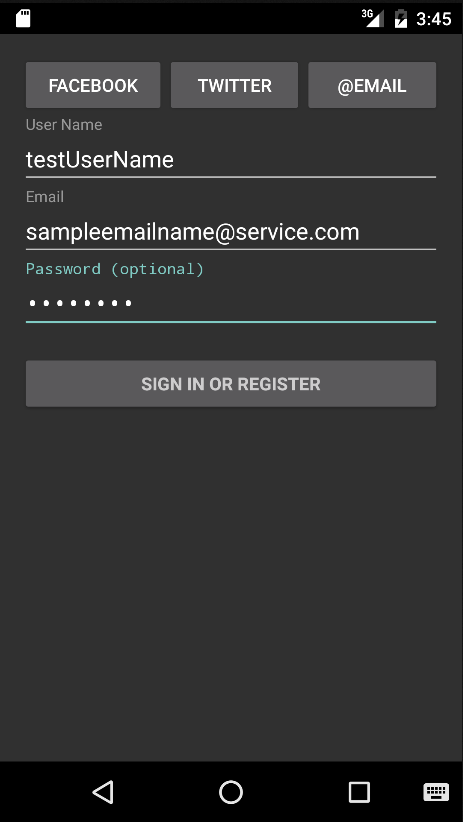
\includegraphics[scale=.4]{Additional/Android/AndroidPictures/loginScreen.png}}
	\end{center}
	\caption{Android login screen \label{AndroudLoginScreen}}
	\end{figure}

	\begin{figure}[tbh]
	\begin{center}
	\fbox{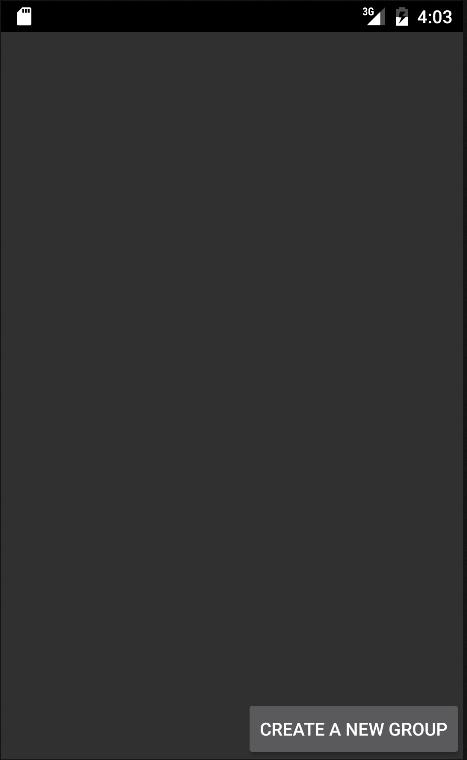
\includegraphics[scale=.4]{Additional/Android/AndroidPictures/createNewGroup.png}}
	\end{center}
	\caption{Android create group screen \label{AndroidCreateGroup}}
	\end{figure}

	\begin{figure}[tbh]
	\begin{center}
	\fbox{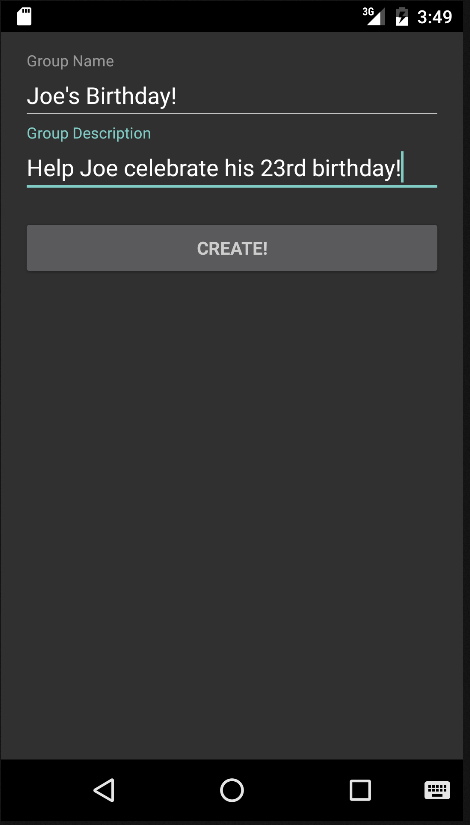
\includegraphics[scale=.4]{Additional/Android/AndroidPictures/groupCreatePage.png}}
	\end{center}
	\caption{Android group information screen \label{AndroidGroupInfo}}
	\end{figure}

	\begin{figure}[tbh]
	\begin{center}
	\fbox{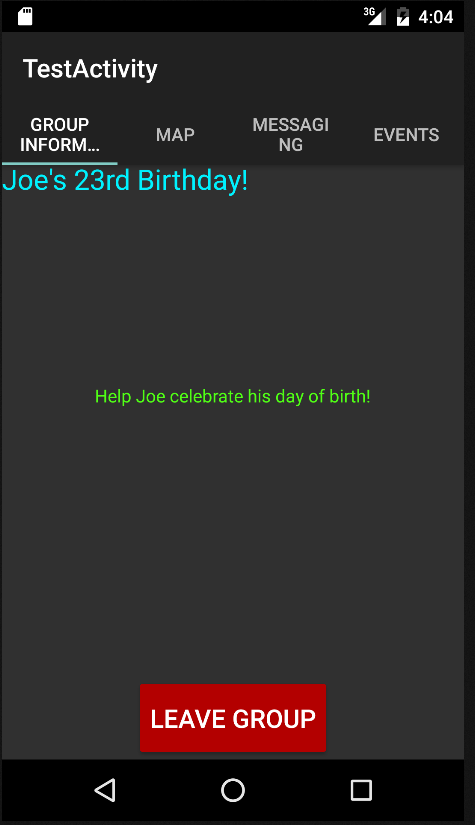
\includegraphics[scale=.4]{Additional/Android/AndroidPictures/groupJoinedPage.png}}
	\end{center}
	\caption{Android group join screen \label{AndroidJoinGroup}}
	\end{figure}

	\begin{figure}[tbh]
	\begin{center}
	\fbox{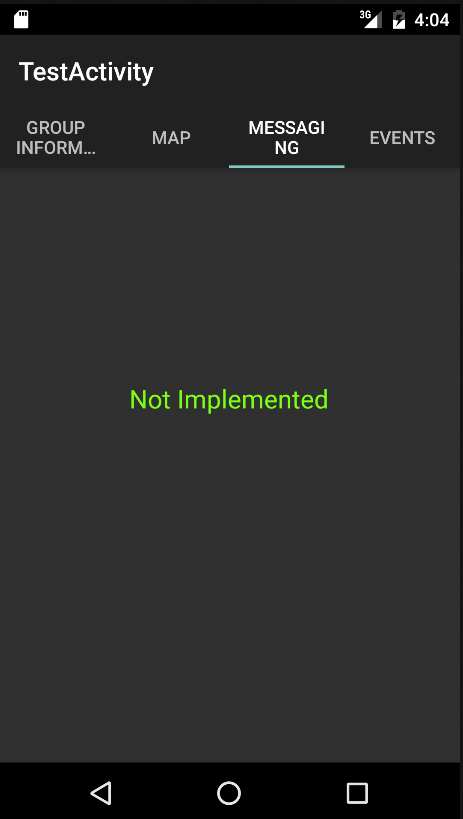
\includegraphics[scale=.4]{Additional/Android/AndroidPictures/messagingNotImplemented.png}}
	\end{center}
	\caption{Android messaging main screen \label{AndroidMessagingMain}}
	\end{figure}


\section{Supporting Material}


%This document might contain references or supporting material which should be documented 
%and discussed  either here if appropriate or more often in the appendices at the end.  This material may have been provided by the stakeholders  
%or it may be material garnered from research tasks.

  %% All tracks (minimal for research track)
% !TEX root = DesignDocument.tex


\chapter{Project Overview}
This section provides some housekeeping type of information with regard to the 
team, project, environment, etc.
Outlined within this section are details involving the development of Crowd Control.  This chapter includes details about the team organization and structure.  Further included is information outlining the financial aspects and the 



\section{Team Member's Roles}
Each team member plays a pivitol role in the development of Crowd Control.  Listed below are each members and their corresponding responsibilities within the production of Crowd Control.  Some of the duties of each member changed half way through production as development of iOS was halted for more progress on Android.  The entire projects duties are outlined below for each individual developer.  

Johnathan Ackerman - Johnathan is leading the front end design and messaging implementation for the Android version of Crowd Control. This entails: 
	\begin {enumerate}
	\item Creating and designing GUI elements for android
	\item Designing messaging Layout
	\item Implementing logic behind group join, group info, and messaging views for Android
	\end{enumerate}

Daniel Andrus - Daniel for the first half was leading the Gui design ad implementation for the iOS version of Crowd Control.  During the second half he worked with Johnathan on Messaging as well as creating our background service. This entails:
	\begin {enumerate}
	\item Creating and designing GUI elements for iOS.
	\item Implementing logic behind group join, group info, and map views for iOS
	\item Implementing logic behind messaging for Android
	\item Creating and implementing a background group service that checks the server for group data updates
	\end{enumerate}

Charles Bonn - Charles is leading the database side of Crowd Control. This database is for both iOS and Android versions. This entails:
	\begin{enumerate}
	\item Creating and managing database queries 
	\item Creating Cloud Code to manage database information
	\item Database load testing
	\end{enumerate}
Charles is also working on future encryption of data going to and from the database.
\newline

Evan Hammer - Evan is leading the back end side for the iOS version of Crowd Control. This entails:
	\begin{enumerate}
	\item Creating links from the database to the mobile application
		\begin{enumerate}
		\item Login link
		\item Group Join Link
		\item Group Member
		\end{enumerate}
	\item Creating links to Apple maps to the mobile application
	\end{enumerate}

Joseph Mowry - Joseph is leading the back end side for the android version of Crowd Control. This endtails:

	\begin{enumerate}
	\item Creating links from the database to the mobile application
		\begin{enumerate}
		\item Login link
		\item Group Join Link
		\item Group Member
		\end{enumerate}
	\item Creating links to Apple maps to the mobile application
	\end{enumerate}



\section{Project  Management Approach}
This section will provide an explanation of the basic approach to managing the 
project.  Typically, this would detail how the project will be managed through 
a given Agile methodology.  The sprint length (i.e. 2 weeks) and product backlog 
ownership and location (ex. Trello) are examples of what will be discussed.  An 
overview of the system used to track sprint tasks, bug or trouble tickets, and 
user stories would be warranted. 

Crowd Control was developed using the Agile software development method.  The project was split up into 7 sprints each lasting 3 weeks.  For the first 4 sprints, each sprint was planned out with goals for each sprint.  The last 3 sprints had plans for each week, creating goals for all of the weeks inside of the sprints.  To track sprint goals, meeting minutes were used to define each members goals at the beginning of each sprint.


\section{ Stakeholder Information}


This section would provide the basic description of all of the stakeholders for 
the project.  Who has an interest in the successful and/or unsuccessful completion 
of this project? 


\subsection{Customer or End User (Product Owner)}
Who?  What role will they play in the project?  Will this person or group manage 
and prioritize the product backlog?  Who will they interact with on the team to 
drive product backlog priorities if not done directly? 

\subsection{Management or Instructor (Scrum Master)}
Who?  What role will they play in the project?  Will the Scrum Master drive the 
Sprint Meetings? 


\subsection{Investors}
Currently Bowtaps has not sought out investment from external sources, instead the members developing Crowd Control have done so using funding from other sources.  To fund the development of Crowd Control the team has entered into a few competitions with their intellectual property to help generate funds.   The team has competed in the South Dakota Governor's Giant Vision, The Innovation Expo, and the Mines CEO Business Plan competitions to gain capitol to cover their current costs.


\subsection{Developers --Testers}
Who?  Is there a defined project manager, developer, tester, designer, architect, 
etc.? 

\section{Budget}
Describe the budget for the project including gifted equipment and salaries for 
people on the project.

\section{Intellectual Property and Licensing}
The intellectual property Crowd Control is owned by Bowtaps LLC which is currently made up of the team currently developing Crowd Control.  All source code, documentation and presentation materials are protected by copyright.

\section{Sprint  Overview}
If the system will be implemented in phases, describe those phases/sub-phases (design, 
implementation, testing, delivery) and the various milestones in this section. 
 This section should also contain a correlation between the phases of development 
and the associated versioning of the system, i.e. major version, minor version, 
revision. 

All of the Agile decisions are listed here.  For example, how do you order your backlog?   
Did you use planning poker?   

\section{Terminology and Acronyms}
Provide a list of terms used in the document that warrant definition.  Consider 
industry or domain specific terms and acronyms as well as system specific. 

\section{Sprint Schedule}
Below is a table of dates for each sprint.\\
\begin{center}
	\begin{tabular}{|c|c|}
	\hline
	Sprint & Date\\
	\hline
	Sprint 1 & 1/18/2016 - 2/5/2016\\
	\hline
	Sprint 2 & 2/15/2016 - 3/4/2016\\
	\hline
	Sprint 3 & 3/21/2016 - 4/15/2016\\
	\hline
	Sprint 3.5 & Time\\
	\hline
	Sprint 4 & 1/18/2016 - 2/5/2016\\
	\hline
	Sprint 5 & 2/15/2016 - 3/4/2016\\
	\hline
	Sprint 6 & 3/21/2016 - 4/15/2016\\
	\hline
	\end{tabular}
\end{center}

\section{Timeline}
Below is an overview of the timeline of the project by sprint.
\begin{center}
	\begin{tabular}{c|c|c}
	Sprint & Tasks & Date\\
	\hline
	Sprint 1 &  Design UX & End of Sprint 1\\
	& Design Database&End of Sprint 1\\
	& Design Application Layers & End of Sprint 1\\
	& Set up GitHub repository & End of Sprint 1\\
	\hline
	Sprint 2 & Code UX & End of Sprint 2 \\
	& Create Models & End of Sprint 2\\
	& Research public/private key passing & End of Sprint 2\\
	\hline
	Sprint 3 & iOS Login & End of Sprint 3\\
	& iOS Facebook integration & End of Sprint 3\\
	& Mapping & End of Sprint 3\\
	& Work on Group Join & End of Sprint 3\\
	\hline
	Sprint 4 & thing & Thing\\
	\hline
	\end{tabular}
\end{center}

\section{Backlogs}
Place the sprint backlogs here.    The product backlog will be in the chapter with the user 
stories.
\subsection{Sprint 1 Backlog}
	\begin{itemize}
	\item Design UX
		\begin{enumerate}
		\item Create groups
		\item Leave groups
		\item Group messaging
		\item Start page
		\end{enumerate}
	\item Database
		\begin{enumerate}
		\item Design database schema
		\item Implement database on Parse
		\end{enumerate}
	\item Design application layers ( MVC )
	\item Set up GitHub repository
	\end{itemize}
	
\subsection{Sprint 2 Backlog}

	\begin{itemize}
	\item Code UX
		\begin{enumerate}
		\item Mapping features
		\item Messaging UI
		\end{enumerate}
	\item Model
		\begin{enumerate}
		\item User Model
		\item Communication Layer
		\item Link back-end and front end
		\end{enumerate}
	\item Implement Cloud code
	\item Business Plan

	\end{itemize}
\subsection{Sprint 3 Backlog}
\begin{itemize}
	\item Messaging API
	\item Join Group Implementation
	\item Cloud Code
	\begin{enumerate}
	\item Group Clean Up
	\item User Information Links
	\end{enumerate}
	\item Business Plan
	\begin{enumerate}
	\item South Dakota Giant Vision
	\item SDSM\&T Business Plan Competition
	\end{enumerate}
\end{itemize}

\subsection{Sprint 3.5 Backlog}
\begin{itemize}
	\item iOS
		\begin{enumerate}
		\item Login/Logout
			\begin{enumerate}
			\item Improved login/sign up screens
			\item Logout feature added
			\end{enumerate}
		\item Settings
			\begin{enumerate}
			\item Settings screen implemented
			\item Logout functionality nested in the Settings screen
			\end{enumerate}
		\item Groups
			\begin{enumerate}
			\item Leaving/Joining a group implemented
			\item Basic group operations
			\item Detect if users are in a group
			\end{enumerate}
		\end{enumerate}
		
	\item Android
		\begin{enumerate}
		\item Login
			\begin{enumerate}
			\item Automatic login on startup (from data store)
			\item Login to existing account via email address
			\end{enumerate}
		\item Settings
			\begin{enumerate}
			\item Page layout created and linked from Group Join page
			\item Logout functionality implemented
			\end{enumerate}
		\item Groups
			\begin{enumerate}
			\item Leave button implemented
			\item Tested adding/removing users from groups
			\end{enumerate}
		\end{enumerate}

	\item Misc/Transitional
		\begin{enumerate}
			\item Further documented Android code to prepare for team merge
			\item Android code review with iOS team, to prepare for team merge
		\end{enumerate}

	\end{itemize}
\subsection{Sprint 4 Backlog}

\begin{description}
	\item[Week 1] \hfill
		\begin{itemize}
		\item Android
		\begin{itemize}
			\item Begin implementing Sinch
			\item Create location and messaging views and managers
			\item Design models and manager classes for messaging and location
			\item
		\end{itemize}
		\item Cloud Code
		\begin{itemize}
			\item Group data parsing started
		\end{itemize}
	\end{itemize}
	
  \item[Week 2] \hfill
		\begin{itemize}
		\item Android
		\begin{itemize}
			\item Broadcast/receive messages to/from all members in a group
			\item Create a layout for messaging
			\item Create a MapFragment to display a map
			\item Created buttons overtop the MapFragment to correspond to syncing and homing locations
		\end{itemize}
		\item Cloud code
		\begin{itemize}
			\item Leaving and joining groups handled
			\item Checking existing email upon login (validation)
		\end{itemize}
	\end{itemize}
  
  \item[Week 3] \hfill
		\begin{itemize}
		\item Android
		\begin{itemize}
			\item Retrieve locations of group members, place their locations on the map via pins
			\item Update group settings and data when changed
			\item Update Group members if someone leaves or joins a group
			\item Group messaging unit tests
			\item GPS Location unit tests
		\end{itemize}
		\item Cloud Code
		\begin{itemize}
			\item Returning group information upon changes
			\item Functional Group update indicator complete
			\item Basic group functionality implemented fully (login/logout, join/leave groups, update on change)
		\end{itemize}
	\end{itemize}
\end{description}
\subsection{Sprint 5 Backlog}
\begin{description}
	\item[Week 1] \hfill
		\begin{itemize}
		\item Senior Design Doc
		\begin{itemize}
			\item Do a general revision of the doc
		\end{itemize}
		\begin{itemize}
		\item Business Plan
			\begin{itemize}
			\item Finish business plan for 2016 Governor's Giant Vision Competition
			\end{itemize}
		\end{itemize}
		\item Android
		\begin{itemize}
			\item Model Caching/ Uniformity
			\item Clean up appearance
		\end{itemize}
	\end{itemize}
	
  \item[Week 2] \hfill
		\begin{itemize}
		\item Android
		\begin{itemize}
			\item Clean up the appearance of the app
			\item Display Group Members on group info page
			\item Safe group operations(leaving/joining group)
			\item Loading animations on homing and syncing
		\end{itemize}
		\item Cloud code
		\begin{itemize}
			\item Safe group operations(leaving/joining group)
		\end{itemize}
	\end{itemize}
  
  \item[Week 3] \hfill
		\begin{itemize}
		\item Android
		\begin{itemize}
			\item Integration Testing
			\item Start Alpha Testing
		\end{itemize}
		\item Cloud Code
		\begin{itemize}
			\item test join and leave functionality
		\end{itemize}
	\end{itemize}
\end{description}

\section{Development Environment}
The basic purpose for this section is to give a developer all of the necessary 
information to setup their development environment to run, test, and/or develop. 
To develop Crowd Control the team used a few differetn products to develop, test, and run.  For development of Crowd Control for Android, the team used the Android Studio IDE which supports all aspects of Android development.  Using Android Studio's Layout Editor to help create the GUI, and using its built in support for Java to code the controller and model layers.  The iOS development all took place on XCode, an Apple Development IDE, much like Android Studio

\section{Development IDE and Tools}
Describe which IDE and provide links to installs and/or reference material. 

\section{Source  Control}
Which source control system is/was used?  How was it setup?  How does a developer 
connect to it? 

\section{Dependencies}
Describe all dependencies associated with developing the system. 

\section{Build  Environment}
How are the packages built?  Are there build scripts? 

\section{Development Machine Setup}
If warranted, provide a list of steps and details associated with setting up a 
machine for use by a developer. 


   %% All tracks

% !TEX root = DesignDocument.tex

\chapter{Design  and Implementation}
This section is used to describe the design details for each of the major components 
in the system.    Note that this chapter is critical for all tracks.  Research tracks would do experimental design here where other tracks would include the engineering design aspects.    This section is not brief and requires the necessary detail that 
can be used by the reader to truly understand the architecture and implementation 
details without having to dig into the code.    Sample algorithm:  Algorithm~\ref{alg1}.  This algorithm environment is automatically placed - meaning it floats.   You don't have to worry about placement or numbering.  

\begin{algorithm} [tbh]                     % enter the algorithm environment
\caption{Calculate $y = x^n$}          % give the algorithm a caption
\label{alg1}                           % and a label for \ref{} commands later in the document
\begin{algorithmic}                    % enter the algorithmic environment
    \REQUIRE $n \geq 0 \vee x \neq 0$
    \ENSURE $y = x^n$
    \STATE $y \Leftarrow 1$
    \IF{$n < 0$}
        \STATE $X \Leftarrow 1 / x$
        \STATE $N \Leftarrow -n$
    \ELSE
        \STATE $X \Leftarrow x$
        \STATE $N \Leftarrow n$
    \ENDIF
    \WHILE{$N \neq 0$}
        \IF{$N$ is even}
            \STATE $X \Leftarrow X \times X$
            \STATE $N \Leftarrow N / 2$
        \ELSE[$N$ is odd]
            \STATE $y \Leftarrow y \times X$
            \STATE $N \Leftarrow N - 1$
        \ENDIF
    \ENDWHILE
\end{algorithmic}
\end{algorithm}
Citations look like~\cite{Choset:2005:PRM, arkin2009governing, lavalle2006}  and~\cite{wiki:asimo,lumelsky:1987, nolfi2000evolutionary}.  These are done automatically.  Just fill in the database {\tt designrefs.bib} using the same field structure as the other entries.  Then pdflatex the document, bibtex the document and pdflatex twice again.  The first pdflatex creates requests for bibliography entries.
The bibtex extracts and formats the requested entries.  The next pdflatex puts them in order and assigns labels.  The final pdflatex replaces references in the text with the assigned labels.
The bibliography is automatically constructed.  
 
 \section{Architecture and System Design}
 This is section will detail the overall system design and general architecture of Crowd Control. The software was designed in such a way that minimizes dependency from third-party services such as Sinch and Parse.
 
 \subsection{Design Selection}
Sprint 1 was centered around designing of the database schema and the general system architecture. Bowtaps produced various high-level designs on both the front-end and back-end of the system that were deeply inspected before deciding on our current implementation.

\subsubsection{Early Design Ideas}
The original database design for Crowd Control consisted of three tables with associated data. Though this design provided a good sense of direction and foundation to build upon, it eventually would need to expand as Crowd Control's feature set expanded. See Figure~\ref{EarlyDBSchema} below.

	\begin{figure}[tbh]
	\begin{center}
	\fbox{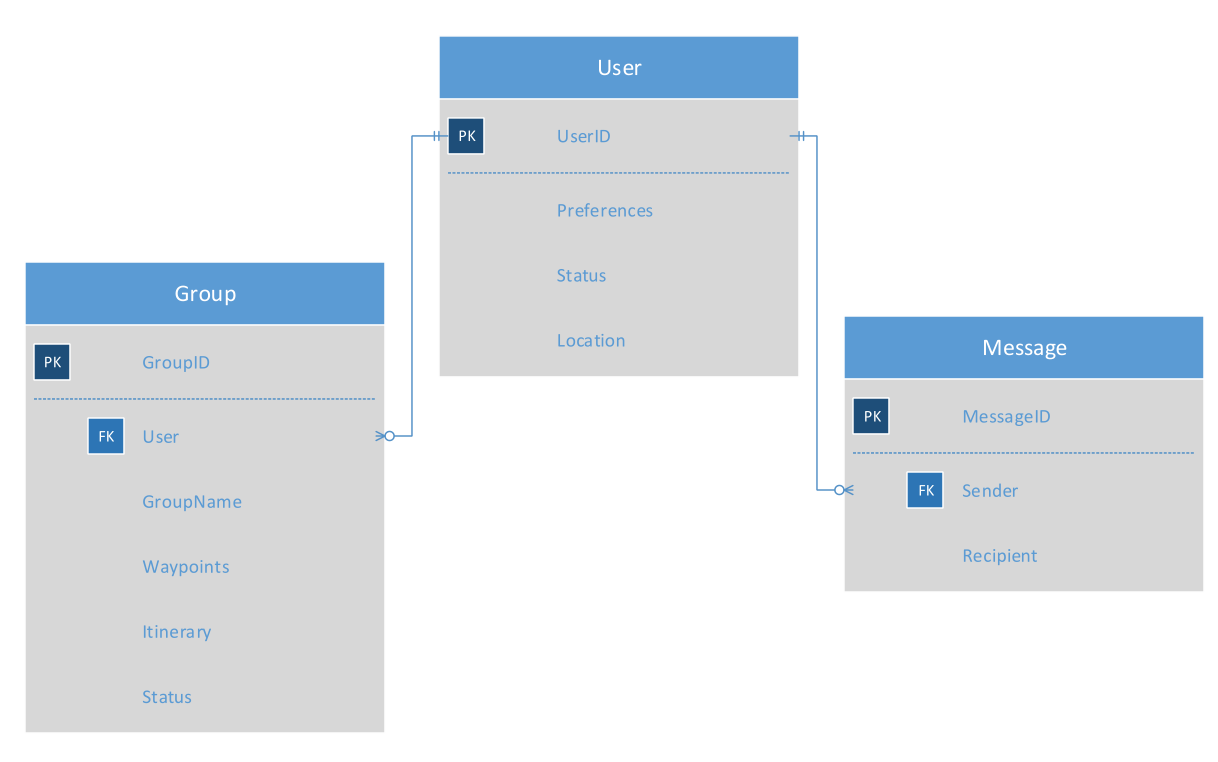
\includegraphics[scale=.5]{Additional/DesignPictures/CC_dbSchema1.PNG}}
	\end{center}
	\caption{Early database schema. \label{EarlyDBSchema}}
	\end{figure}

Another caveat to this design is the failure to differentiate between public and private user data. In Crowd Control, each user has data that is private to that user, such as their email and password. However, there is also a set of public data that can be viewed by other users, such as their display name or their location. This iteration of the schema only has one user entity, that stores their information. A small lack of understanding about Parse's no-SQL implementation lead us to improperly design our entities in this way. It was later deemed that this separation between front-facing and hidden user data entities was necessary in terms of ease-of-access and information privacy.

\subsubsection{Improvements to Early Designs}
In reflection of the shortcomings of the first design iteration, the database schema was restructured to better fit Crowd Control's needs. The current design consists of eight data tables,  shown in Figure~\ref{MidDBSchema} below. More entities were added to the overall schema. One such addition was a ``CCUser'' table to hold the public data associated with a user. It is important to note that the ``User'' table was left to hold a user's private data. Those changes and some additions resulted in the below schema. 

	\begin{figure}[tbh!]
	\begin{center}
	\fbox{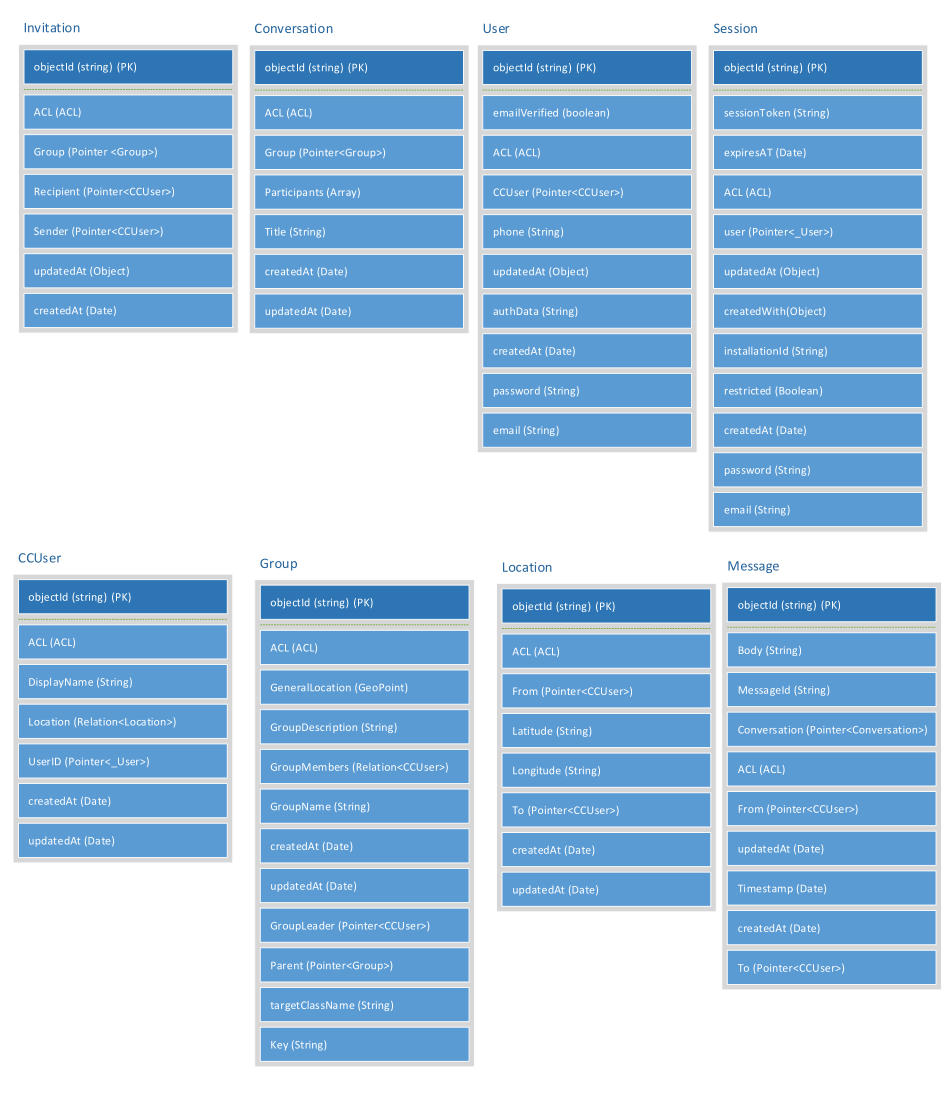
\includegraphics[scale=.65]{Additional/DesignPictures/CC_dbSchema2.PNG}}
	\end{center}
	\caption{Improved database schema. \label{MidDBSchema}}
	\end{figure}

 \subsection{Data Structures and Algorithms}
 TODO: Model classes and hierarchy? Perhaps irrelevant (see ``Classes below'')
 
 \subsection{Data Flow}
 TODO: Create Data Flow diagram of overall process
 
 
 \subsection{Communications}
 One of the core features to the Crowd Control app is communication amongst its users. To achieve this, some third-party services are used, which in turn communicate data between users. If a user wishes to send another user a message, that message is sent to the Parse back-end, and delivered to the recipient via the Sinch service. The basic communication overview is outlined below in Figure ~\ref{CommFlow}.
 
  	\begin{figure}[tbh]
	\begin{center}
	\fbox{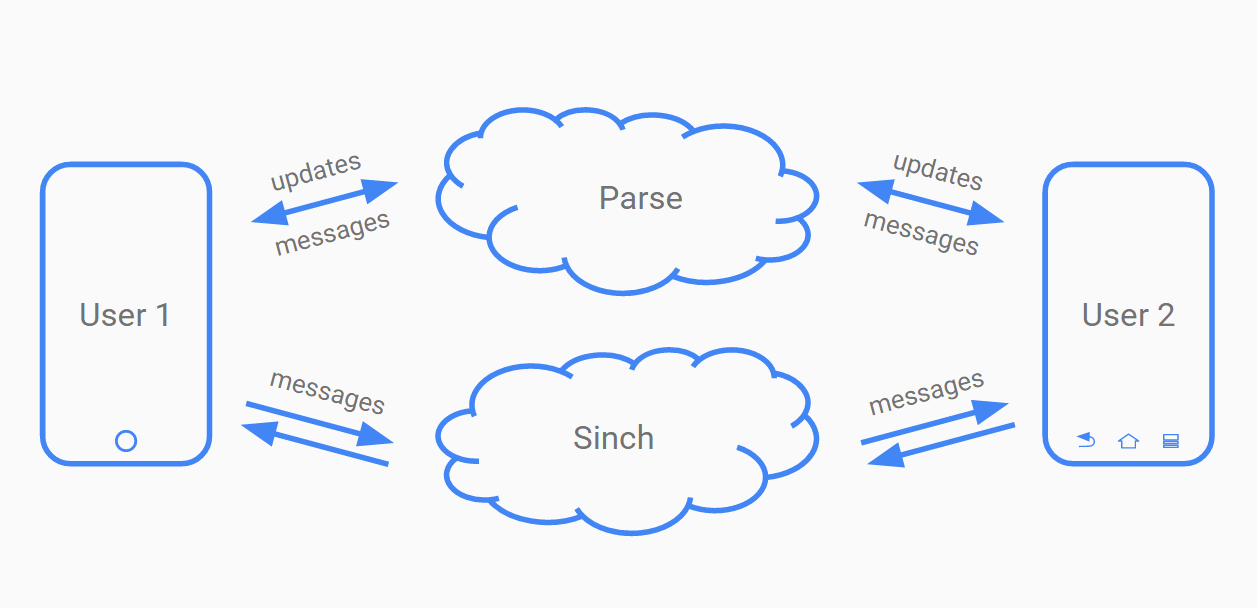
\includegraphics[scale=.5]{Additional/DesignPictures/CommFlow.PNG}}
	\end{center}
	\caption{Communication flow diagram. \label{CommFlow}}
	\end{figure}
 
 In addition to message-passing, various other data is being transfered from the users' devices. One such example is GPS data. Upon retrieval of a user's location, that value is stored in Parse, and able to be fetched by any group member that wishes to see that location. 

 \subsection{Classes}
 TODO: Include class hierarchy (models, base models, interfaces)
 \subsection{UML}
 TODO: UML diagram...can Android studio generate these via a plugin?
 
 \subsection{GUI}
 TODO: Overview of GUI design. Show differences in platform native ``look and feel''
 
 \subsection{MVVM, etc}
 TODO: Describe MVVM, create diagram laying our components in MVVM format

\section{Group Messaging }

\subsection{Technologies  Used}
\begin{itemize}
  \item Parse
  \item Sinch
\end{itemize}

\subsection{Component  Overview}
\begin{itemize}
  \item Send/receive messages to/from group members (many-to-many)
  \item Store messages in Parse (data persistence)
  \item Message transfer service is independent of carrier/device/platform
\end{itemize} 

\subsection{Phase Overview}
This is an extension of the Phase Overview above, but specific to this component. 
 It is meant to be basically a brief list with space for marking the phase status. 

\subsection{Architecture Diagram}
It is important to build and maintain an architecture diagram.  However, it may 
be that a component is best described visually with a data flow diagram. 

\subsection{Data Flow Diagram}
It is important to build and maintain a data flow diagram.  However, it may be 
that a component is best described visually with an architecture diagram. 

\subsection{Design Details} - NOTE: Code block probably irrelevant here. Will remove later.
This is where the details are presented and may contain subsections.   Here is an example code listing:
\begin{lstlisting}
#include <stdio.h>
#define N 10
/* Block
 * comment */
 
int main()
{
    int i;
 
    // Line comment.
    puts("Hello world!");
 
    for (i = 0; i < N; i++)
    {
        puts("LaTeX is also great for programmers!");
    }
 
    return 0;
}
\end{lstlisting}
This code listing is not floating or automatically numbered.  If you want auto-numbering, but it in the algorithm environment (not algorithmic however) shown above.

\section{Location Tracking }

\subsection{Technologies  Used}
\begin{itemize}
  \item Google Play Services / Apple Map Features
  \item Parse
\end{itemize}

\subsection{Component  Overview}
\begin{itemize}
  \item Track all group members in a map fragment
  \item Homing functionality on the user's location pin
  \item Sync group locations automatically (interval-based) and manually (on button-press)
\end{itemize}

\subsection{Phase Overview}
This is an extension of the Phase Overview above, but specific to this component. 
 It is meant to be basically a brief list with space for marking the phase status. 

\subsection{ Architecture  Diagram}
It is important to build and maintain an architecture diagram.  However, it may 
be that a component is best described visually with a data flow diagram. 

\subsection{Data Flow Diagram}
It is important to build and maintain a data flow diagram.  However, it may be 
that a component is best described visually with an architecture diagram. 


\subsection{Design Details}
This is where the details are presented and may contain subsections. 

\section{Group Management }

\subsection{Technologies  Used}
\begin{itemize}
  \item Parse
\end{itemize}

\subsection{Component  Overview}
\begin{itemize}
  \item Store group members in a group
  \item Incorporate a party leader to manage the group (has special priveledges)
  \item Create a group with specific attributes that can be changed by the leader
\end{itemize}

\subsection{Phase Overview}
This is an extension of the Phase Overview above, but specific to this component. 
 It is meant to be basically a brief list with space for marking the phase status. 

\subsection{ Architecture  Diagram}
It is important to build and maintain an architecture diagram.  However, it may 
be that a component is best described visually with a data flow diagram. 


\subsection{Data Flow Diagram}
It is important to build and maintain a data flow diagram.  However, it may be 
that a component is best described visually with an architecture diagram. 


\subsection{Design Details}
This is where the details are presented and may contain subsections. 


  %% All tracks
% !TEX root = DesignDocument.tex


\chapter{System and Unit Testing}

Crowd Control utilizes multiple sevices across different platforms, requiring
all parts to be operating correctly in order to provide consistent service to
all users. We use system and unit testing to assist developers in identifing 
potential issues and to verify that the product being produced meets
requirements. The goal of system and unit testing is to automate the process to
increase development efficiency and reduce testing errors.

Given the time constraints and scope of Crowd Control, we have been forced to
make compromises in regards to system and unit testing. Implementing and running
automated unit testing, can be as time-consuming as writing production code. In
fact, it is extremely common for a single function of production code to require
many times as many lines of unit testing code to completely test the function.
While automated testing provides many invaluable benefits, it would ultimately be
a hinderance to the project if it means missing critical deadlines and not
achieving crucial project milestones.

In this section, we describe our approach to testing, our goals, and the test
cases that we have developed and implemented thus far. We also discuss the
future plans for testing and how we will be able to devote more time and energy
towards this project in the upcoming months.


\section{Overview}

For this project, we use a combination of ``black-box'' and ``white-box''
testing. This means that there are some aspects of the project that we have
created ourselves and have full control over its execution, and there are others
that we have little control over because it is was provided by a third party.
In practical terms, it means that we can test our own code with the full
knowledge of how it is intended to work, allowing us to design tests that target
potential problem areas. When designing tests that make use of a third-party
service or a library that we have not written ourselves, we can only write tests
that verify that the supplied functionality works as documented.

Because one of the goals of this project is to develop the applications using
native languages and technology, we make use of the most established testing
frameworks for the platform we are testing on. For the iOS application, we use
the testing tools and frameworks built directly into Xcode. For the Android
application, we use Espresso for testing our interface and JUnit for testing our
classes and methods. To test Parse, the third party service we use for data
storage and retrieval, we use unit testing on both Android and iOS, as
interacting with Parse requires a running application on a device. To test
Sinch, the third party service we use for instant messaging between users, we
use the unit testing frameworks we use for testing our Android and iOS
applications since interacting with Sinch also requires a running instance of
the application on a device.

Running unit tests in all of the frameworks above yields a list of binary
results; for each test executed, we receive either a ``pass'' or ``fail''
result. If a test fails, we may also receive a message describing the issue
that caused the test to fail. There exist several conditions that could cause
a test to fail.

\begin{itemize}
	\item An uncaught exception is thrown
	\item A runtime error is encountered
	\item The application crashes
	\item A test assertion fails
\end{itemize}

When designing test cases, we begin with the set of user stories identified at
the beginning of the project. A list of user stories can be found in the section
\ref{userStories}. From these user stories, we build a testing matrix that will
be referenced when writing our automated tests. Tests are then written as the
code they are intended to test is written.

Tests are also to be run relatively frequently. Ideally, developers would enable
the set of tests relevant for the aspect of the project they are currently
working on and run those tests as needed during development and again before the
code is merged in with the rest of the project. Then, the full set of tests
would be run automatically and at a time that would not interfere with
development or execution of the product.


\section{Dependencies}

This project can be broken into several pieces that all work together to form a
single cohesive product. Taken individually, these pieces would be of little
utility. It is important that we test each how well each component interacts
with each other as well as each isolated part as best we can. The four main
components of this project are as follows:

\begin{itemize}
	\item Android client application
	\item iOS client application
	\item Parse service and cloud code
	\item Sinch service
\end{itemize}

Each of these aspects of the project need to be somehow tested, although some
parts can be more accurately tested than others. More thorough requirement
breakdowns of each aspect are described in the subsections below.


\subsection{Android Client Application}

To test our client code running locally on Android devices, we use two testing
frameworks: JUnit for testing Android-independent code and Espresso for testing
navigation and user interface requirements. These frameworks are run from within
our integrated development environment, Android Studio. Additionally, for
interface testing, we require a running emulator or a connected Android device on
which Android Studio can run the unit tests.

While developing unit tests for the JUnit and Espresso frameworks, we use
\href{https://google.github.io/android-testing-support-library/docs/index.html}
{Google's Android testing Support Library Documentation} website. This resource
provides accurate information on installing and using these frameworks in
conjunction with Android Studio. Writing unit tests and best practices, as well
as class documentation are available from this website.


\subsection{iOS Client Application}

To test our client code running locally on iOS devices, we use the testing tools
included in Xcode, our iOS integrated development environment. Backend unit
testing and interface testing are all handled by the same framework. These tests
are run from within Xcode. Interface tests require a running iOS emulator or an
iOS device connected to the computer. Because the unit testing tools used to
test iOS devices are tied to Xcode, this means that the tests can only be run on
a Macintosh computer.

While developing unit tests for iOS devices, we reference \href{https://developer.apple.com/library/ios/documentation/ToolsLanguages/Conceptual/Xcode_Overview/UnitTesting.html}
{iOS Developer Library} website. This resource contains instructions on
designing and setting up unit tests, as well as instructions on running unit
tests. Class documentation can also be found on this website.


\subsection{Parse Service and Cloud Code}

Some aspects of our project exist as ``cloud code'', which is custom server-side
logic executed by our database backend service, Parse. This cloud code is
written in JavaScript and handles database operations that require security,
data integrity, consistency, and efficency. However, because this cloud code
runs on a remote server to which we have limited access and concealed knowledge
of its internal workings, we are forced to test the our code by the only means
we have; using the client applications.

Parse does not supply testing features, and thus we must devise a way to execute
our own unit tests using the tools we have. To test the functionality of our
cloud code and our Parse interaction code, we require these things:

\begin{enumerate}
	\item The Parse libraries installed
	\item Parse interactivity built into the application
	\item An active Internet connection to the Parse service
	\item An emulator/simulator/developer device
	\item The testing framework associated with the client platform being used
	for testing
	\item A Parse application key
	\item A separate Parse database dedicated to testing
\end{enumerate}

In order to run tests on our cloud code, we use both versions of our client (iOS
and Android) to connect to the Parse server, perform database operations by
calling cloud code, then verifying the results. We use the aforementioned
testing frameworks to develop and execute these tests on both platforms. These
tests can be performed on device simulators, device emulators, and physical
developer devices alike.

When using client software to test server software, we must properly configure
the clients to interact with the database as if it were no different than a
production database. Thus, we require that the Parse libraries be included in
the project and that actual Parse functionality built into the application. As
with all Parse-enabled applications, this requires a unique application key be
assigned by Parse and used to access the database.

Because running tests on Parse result in changes to the data in the database we
are testing with, it is crucial that the automated tests be run on an
independent Parse database dedicated to testing. Running such tests on either
the production or development databases could result in irreversable destruction
of data that we cannot afford to jeapordize. In order to avoid this, all unit
tests that involve testing Parse functionality should be executed using a
database where the data is used exclusively for testing.


\subsection{Sinch Service}

Another crucial third party service we utilize is Sinch, an instant messaging
platform that we use in conjunction with Parse. This service does not have cloud
code support, but that is okay since we have no need for cloud code here.
However, it is important that we test how well our client applications connect
to and use the service to ensure that communications run smoothly.

In order to test the functionality of Sinch and how well our applications
interact with it, we require these things:

\begin{enumerate}
	\item The Sinch libraries installed
	\item Sinch functionality built into the application
	\item An active internet connection to Sinch
	\item An emulator/simulator/developer device running the application
	\item The testing framework associated with the client platform being used
	for testing
	\item A Sinch application key
	\item A separate Sinch application dedicated to testing
\end{enumerate}

As with Parse, Sinch is a third party service to which we have limited access
and no knowledge of the implementation details. With the addition of the fact
that we have no cloud code for Sinch to test, the only aspect of this service we
need to test is how our client applications interact with the service.

To test our integration with Sinch, we run tests using our Android and iOS
client applications on either device emulators, device simulators, or physical
development devices. To develop and run these tests, we use the aforementioned
testing frameworks used for testing the client code itself on each platform.
We then run our tests on these devices, which cause the application to connect
to and communicate with Sinch using the provided developer API. Sinch requires
an active Internet connection, so the success of the tests depends on the
testing devices having a stable Internet connection.

Lastly, like Parse, Sinch supplies a unique application key which our clients
use to authenticate with the Sinch servers. All versions of our client
applications use this key and is what allows them to communicate with each
other. Also like Parse, we require that all tests run through Sinch also be run
using a special Sinch application key that is completely separate from the
production and development versions of the application. We must do this in order
to avoid user ID conflicts and to limit any operations that may affect service
uptime and reliability.


\section{Test Setup and Execution}
Describe how test cases were developed, setup, and executed.  This section can 
be extremely involved if a complete list of test cases was warranted for the system.   One 
approach is to list each requirement, module, or component and describe the test.

The unit tests are described here.

\section{System Testing}

\section{System Integration Analysis}

\section{Risk Analysis}

\subsection{Risk Mitigation}

\section{Successes, Issues and Problems}

During the course of our project's development, we have encountered various
successes, issues, and problems in regards to system and unit tesing. Details on
each of these are listed below, along with a summary on the changes made to our
testing backlog throughout the course of this project.


\subsection{Successes}

The greatest success of our work in unit and system tesing has been in the
development of our testing matrix. Our tesing matrix, while not comprehensive
(as such a matrix requires years of refining to produce), will act as a set of
blueprints when setting up automated tests. At over one hundred test cases
strong, this matrix defines the behavior of our application in many different
possible states. Using this information, we can implement automated unit tests
more efficiently than if we did not have such a matrix.

A secondary success in our testing efforts was in discovering that all of the
necessary tesing frameworks are free and are mature enough to have exhaustive
documentation and support. We have access to a plethora of information that has
aided us in designing and implementing unit and system tests using these native
tools. Additionaly, the tools we are using integrate seamlessly into the IDEs we
are using for development, reducing the number of tools required to use them.

Finally, we have succeeded in designing and implementing a number of unit tests
for both iOS and Android versions of our client applications. As implementing
unit tests takes a significant time investment, the ones we have built provide a
good foundation upon which to build. On iOS for example, many interface tests
related to the login and signup screens have been implemented and are used for
tesing account creation and login. On Android, we have implemented a similar set
of unit tests as we did for iOS.


\subsection{Issues}

One major issue we encountered when designing unit tests was the fact that none
of the team members have had significant experience doing so. Although a number
of us have had a moderate amount of formal education on the subject through
couse and guest lectures, none have designed or implemented automated tesing in
a project of this magnitude. Thus, an enormous part of testing for this project
was devoted to studying testing methods used in other projects and researching
how to use our tools to build these tests.

The second issue encountered was time constraints. Our goals to turn this
project into a viable product fit for the market required that we focus heavily
on progress towards a working prototype that can be demonstrated by the end of
the semester. Automated tesing, although an important development tool, requires
a large time investment overhead that we could not afford if we desired to meet
requirement deadlines and achieve our critical milestones.

When making the concious decision to prioritize our efforts, we agreed that code
separability and maintainability should not be neglected. These two tennants of
software development are heavilty promoted by automated tesing. By choosing to
prioritize separability and maintainability when designing our software, we are
confident that delaying automated tesing will be less of a hurdle when the time
comes to implement them. Regardless, we are aware that by not investing the time
now, we are accruing ``technical debt'', which means that this task will be more
difficult to accomplish the longer we delay.


\subsection{Problems}

The unit and system testing section of this project was not without its own set
of problems. Many of these we did not forsee, as they are problems that have
arisen from our tools or our tesing devices, both of which we have limited
control over.

Xcode, the IDE chosen for iOS development underwent an update that apeared to
cause UI tesing on iOS to become undependable. Often unit tests run using this
tool would immediately report failures without apparently running the test
properly. It is possible that this is a configuration error, but it is one that
we have yet to solve if it is. Other Xcode users have reported similar problems
using these features.

Another problem encountered was in using our hardware devices to run automated
tesing. For the most part, the device simulators and emulators are adequate for
running most tests. In some cases, the devices would not cooperate with the
testing frameworks. These devices would either run too slowly for the tests and
sometimes reject the incoming connection to the IDE. In the end, we decided to
forego solving these technical difficulties to focus on product development and
business-related issues.


\subsection{Changes to the Backlog}

  %% All tracks
% !TEX root = DesignDocument.tex


\chapter{Prototypes}

This chapter is for recording each prototype developed.  It is a historical record of what you accomplished in 464/465.   This should be organized according to Sprints.  It should have the basic description of the sprint deliverable and what was accomplished.  Screen shots, photos, captures from video, etc should be used.  

\section{Sprint 1 Prototype}
This sprint was focused on learning Android and iOS development tools, as well as designing the UX and the database schema.
\subsection{Deliverable}
	\begin{itemize}
		\item UX for Android
		\item UX for iOS
	\end{itemize}
\subsection{Backlog}
	\begin{itemize}
		\item UX design (MVC)
		\begin{itemize}
			\item Create group
			\item Leave group
			\item Group messaging
			\item Start page
		\end{itemize}
		\item Database
		\begin{itemize}
			\item Design database schema
			\item Implement database on Parse
		\end{itemize}
	\end{itemize}
\subsection{Success/Fail}
\begin{itemize}
	\item Designs for Create Group page
	\item Design for Leave Group page
	\item Design for Group Messaging page
	\item Design for Start Page
	\item Design for Database Schema
	\item Database implementation
	\item Git Repository Initialization
\end{itemize}

\section{Sprint 2 Prototype}

	\begin{figure}[tbh]
	\begin{center}
	\fbox{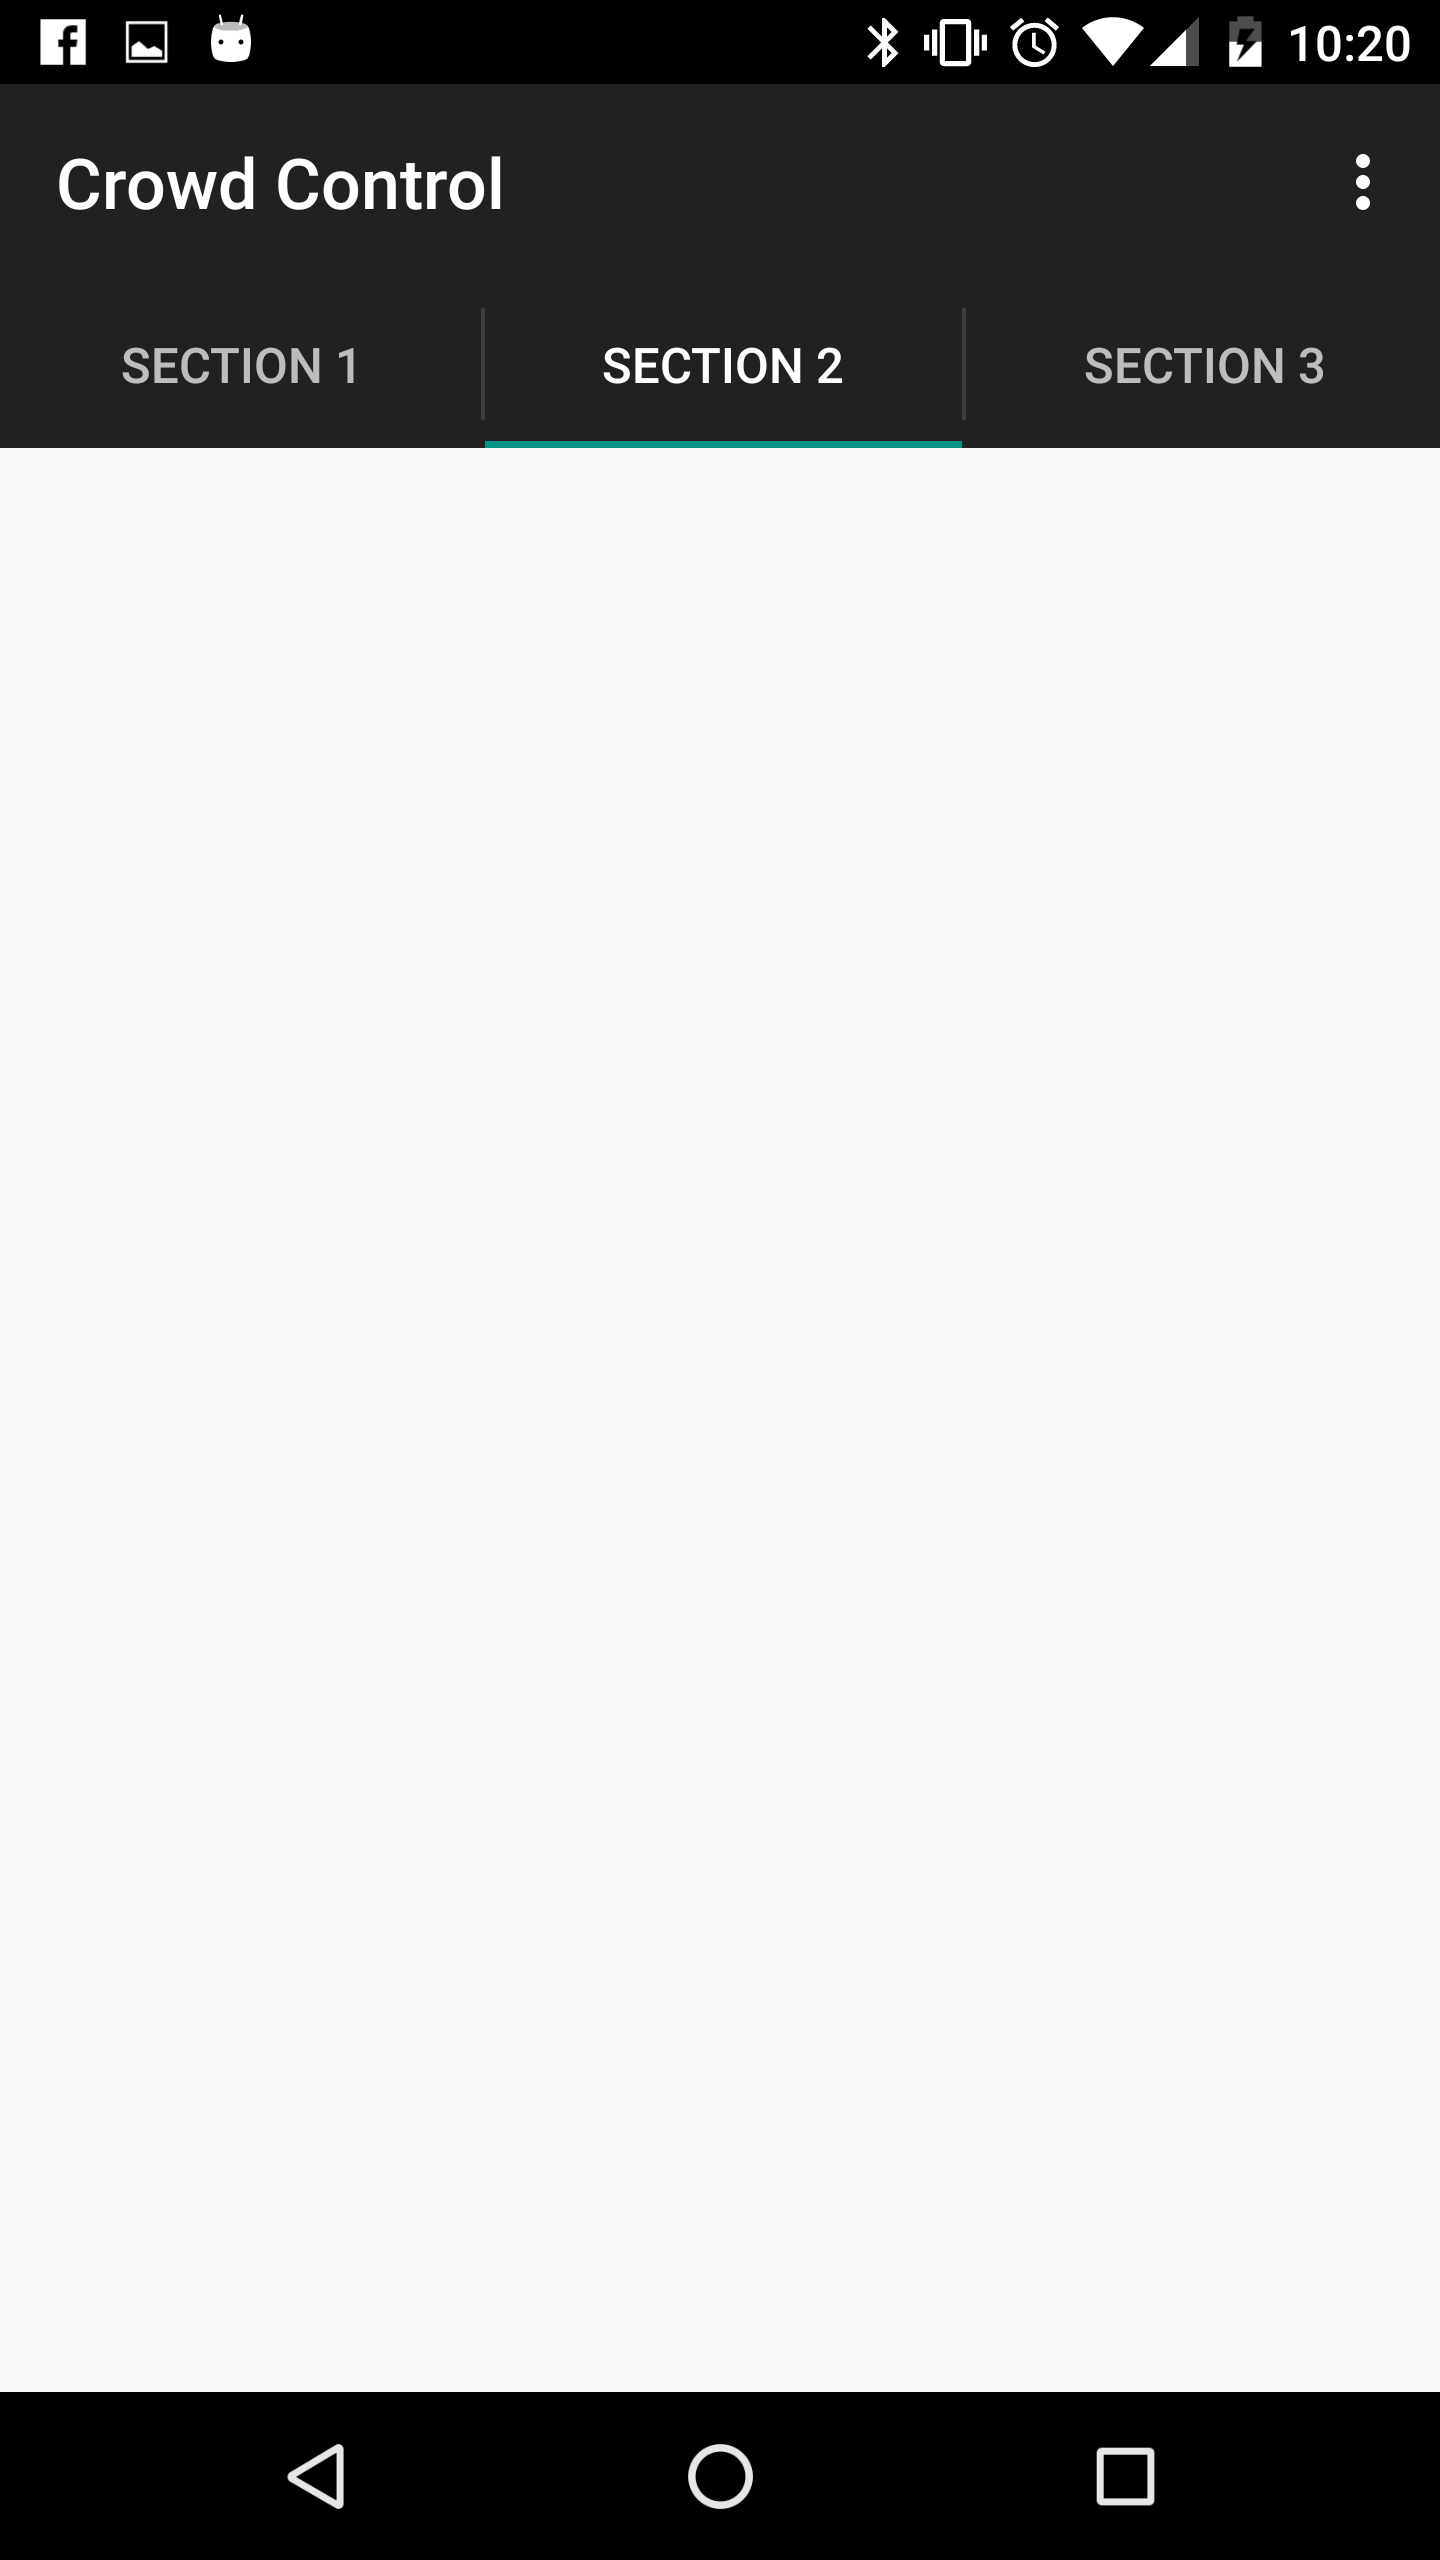
\includegraphics[scale=.1]{Additional/Prototypes/Sprint2/tabs.PNG}}
	\end{center}
	\caption{Sprint 2 Prototypes. \label{CommFlow}}
	\end{figure}

\subsection{Deliverable}
\begin{itemize}
	\item Android
	\begin{itemize}
		\item UX
		\begin{itemize}
			\item Designed map screen
			\item Designed group info screen
			\item Designed start page
			\item Designed group messaging
			\item Created initial tabs holder
		\end{itemize}
		\item Model
		\begin{itemize}
			\item Created skeleton user model
			\item Created skeleton group model
			\item Created skeleton abstractions for models
		\end{itemize}
	\end{itemize}
	\item iOS
	\begin{itemize}
		\item UX
		\begin{itemize}
			\item Created map display
			\item Added homing button to map display
			\item Created simple group display
		\end{itemize}
		\item Model
		\begin{itemize}
			\item Created skeleton user model
			\item Created skeleton profile model
			\item Created skeleton group model
			\item Created skeleton abstractions for models
		\end{itemize}
	\end{itemize}
	\item Parse
	\begin{itemize}
		\item Created User table
		\item Created CCUser table
		\item Created Group table
	\end{itemize}
	\item Work was also done on the Business Plan
\end{itemize}
\subsection{Backlog}
\begin{itemize}
	\item Code UX
	\begin{itemize}
		\item Implement mapping features
		\item Create messaging UI
	\end{itemize}
	\item Model
	\begin{itemize}
		\item Create user Model
		\item Create communication Layer
		\item Link back-end and front end
	\end{itemize}
	\item Create parse tables
	\item Business Plan
\end{itemize}
\subsection{Success/Fail}
\begin{itemize}
	\item We had a hard time finding a version of Public/Private key encryption that fit our project.
	\item Differences between iOS and android coding standards made it hard to create a similar look and feel.
	\item iOS is simply easier to make these initial pieces in, and has jumped far ahead android.
	\item iOS map features are proving very difficult to test.
\end{itemize}

\section{Sprint 3 Prototype}

	\begin{figure}[tbh]
	\begin{center}
	\fbox{\includegraphics[scale=.1]{Additional/Prototypes/Sprint3/createAccount.PNG}}
	\fbox{\includegraphics[scale=.1]{Additional/Prototypes/Sprint3/email.PNG}}
	\end{center}
	\caption{Sprint 3 Prototypes. \label{CommFlow}}
	\end{figure}

\subsection{Deliverable}
\begin{itemize}
	\item iOS
	\begin{itemize}
		\item Created a log-in system
		\begin{itemize}
			\item Added ability to create a user
			\item Added Facebook integration for user creation
		\end{itemize}
		\item Added ability for users to join an existing group
	\end{itemize}
	\item Android
	\begin{itemize}
		\item Added ability to create a user with an email address
		\item Added group functionality
		\begin{itemize}
			\item Added a way for groups to be created
			\item Added a group join feature
		\end{itemize}		
	\end{itemize}
	\item Server
	\begin{itemize}
		\item Fixed connection issues between parse and app
		\item User table and profile(CCUser) are connected by apps in parse
	\end{itemize}
	\item Prepped business plan for SDSM\&T Business Plan Competition
\end{itemize}
\subsection{Backlog}
\begin{itemize}
	\item Install a messaging API
	\item Allow users to join a group
	\item Cloud Code
	\begin{itemize}
		\item Create safe group operations
		\item Link user information
	\end{itemize}
	\item Business Plan
	\begin{itemize}
		\item Submit to SDSM\&T Business Plan Competition
		\item Prep for South Dakota Giant Vision
	\end{itemize}
\end{itemize}
\subsection{Success/Fail}
\begin{itemize}
	\item Failures
	\begin{itemize}
		\item Not all of the group functionality is working properly
		\item We were unable to get to messaging this sprint
	\end{itemize}
	\item Changes
	\begin{itemize}
		\item Rewrote the database schema
		\item Modified GUI appearance
	\end{itemize}
	\item Successes
	\begin{itemize}
		\item iOS was successful in connecting to Facebook
		\item Android managed to start creating groups
		\item Our business plan was accepted by SDSM\&T Business Plan Competition
	\end{itemize}
\end{itemize}

\section{Winter Sprint Prototype}

	\begin{figure}[tbh]
	\begin{center}
	\fbox{\includegraphics[scale=.1]{Additional/Prototypes/SprintW/createAccount.PNG}}
	\fbox{\includegraphics[scale=.1]{Additional/Prototypes/SprintW/email.PNG}}
	\fbox{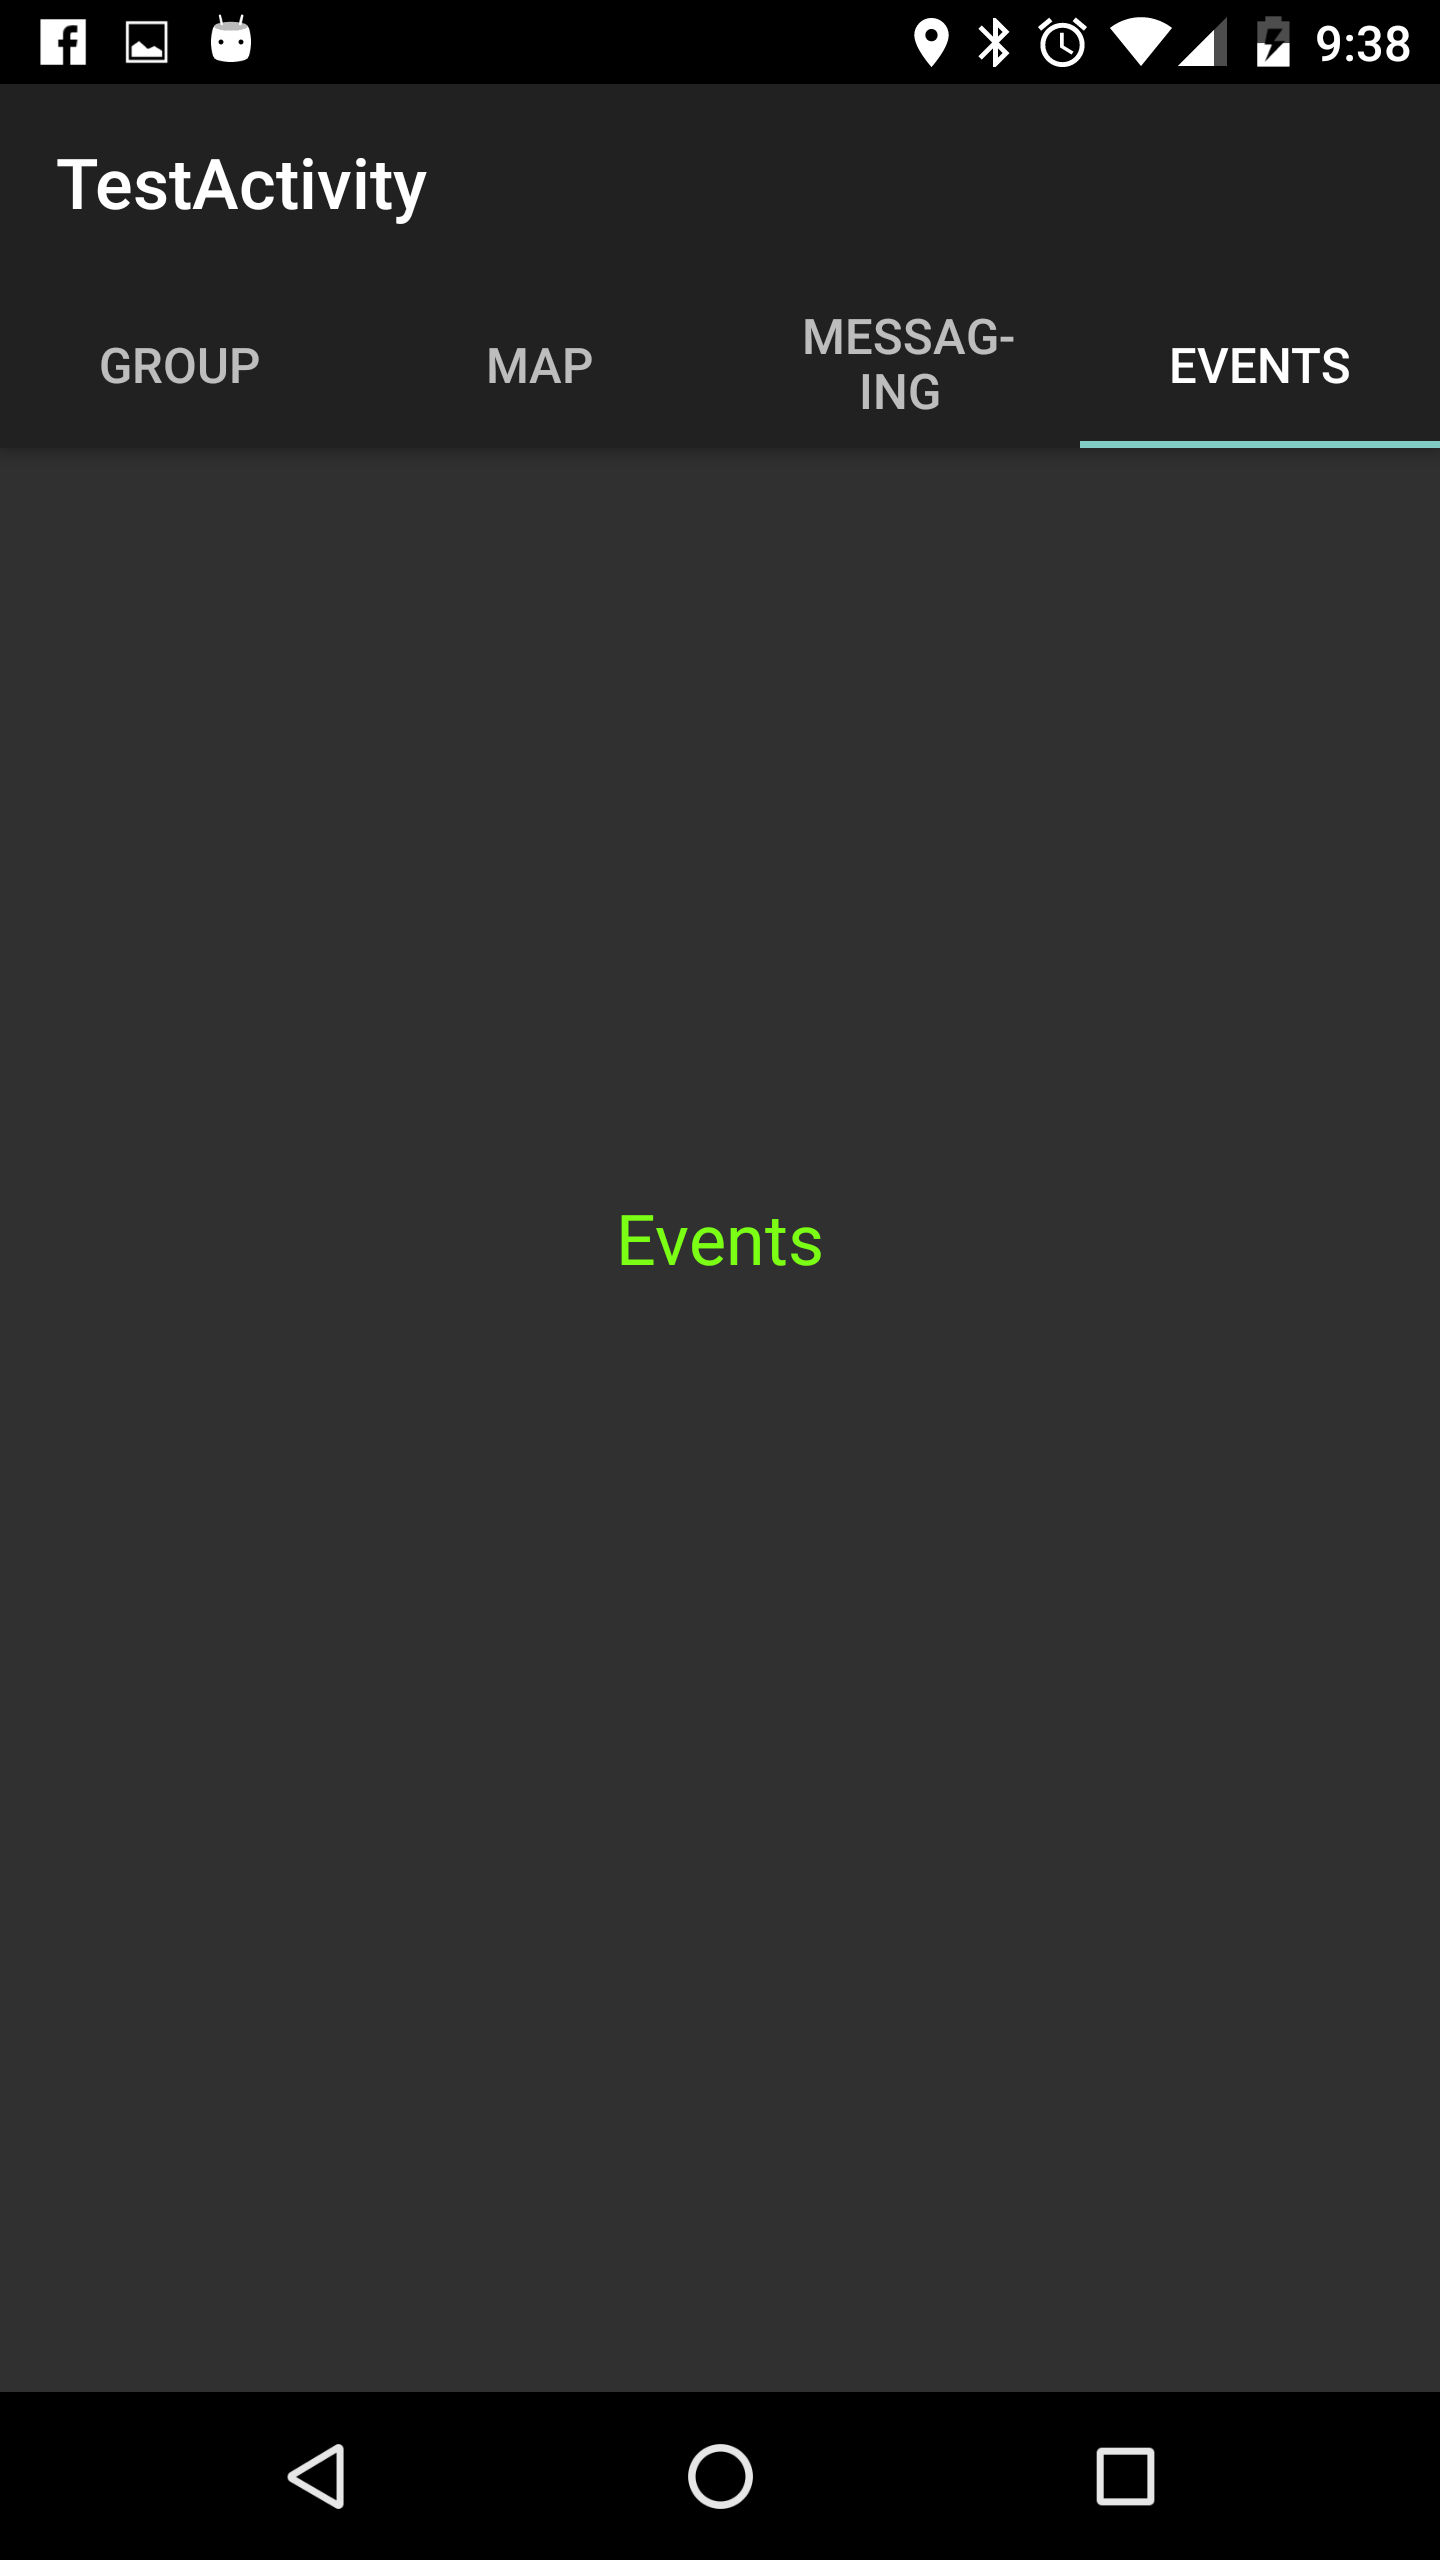
\includegraphics[scale=.1]{Additional/Prototypes/SprintW/events.PNG}}
	\fbox{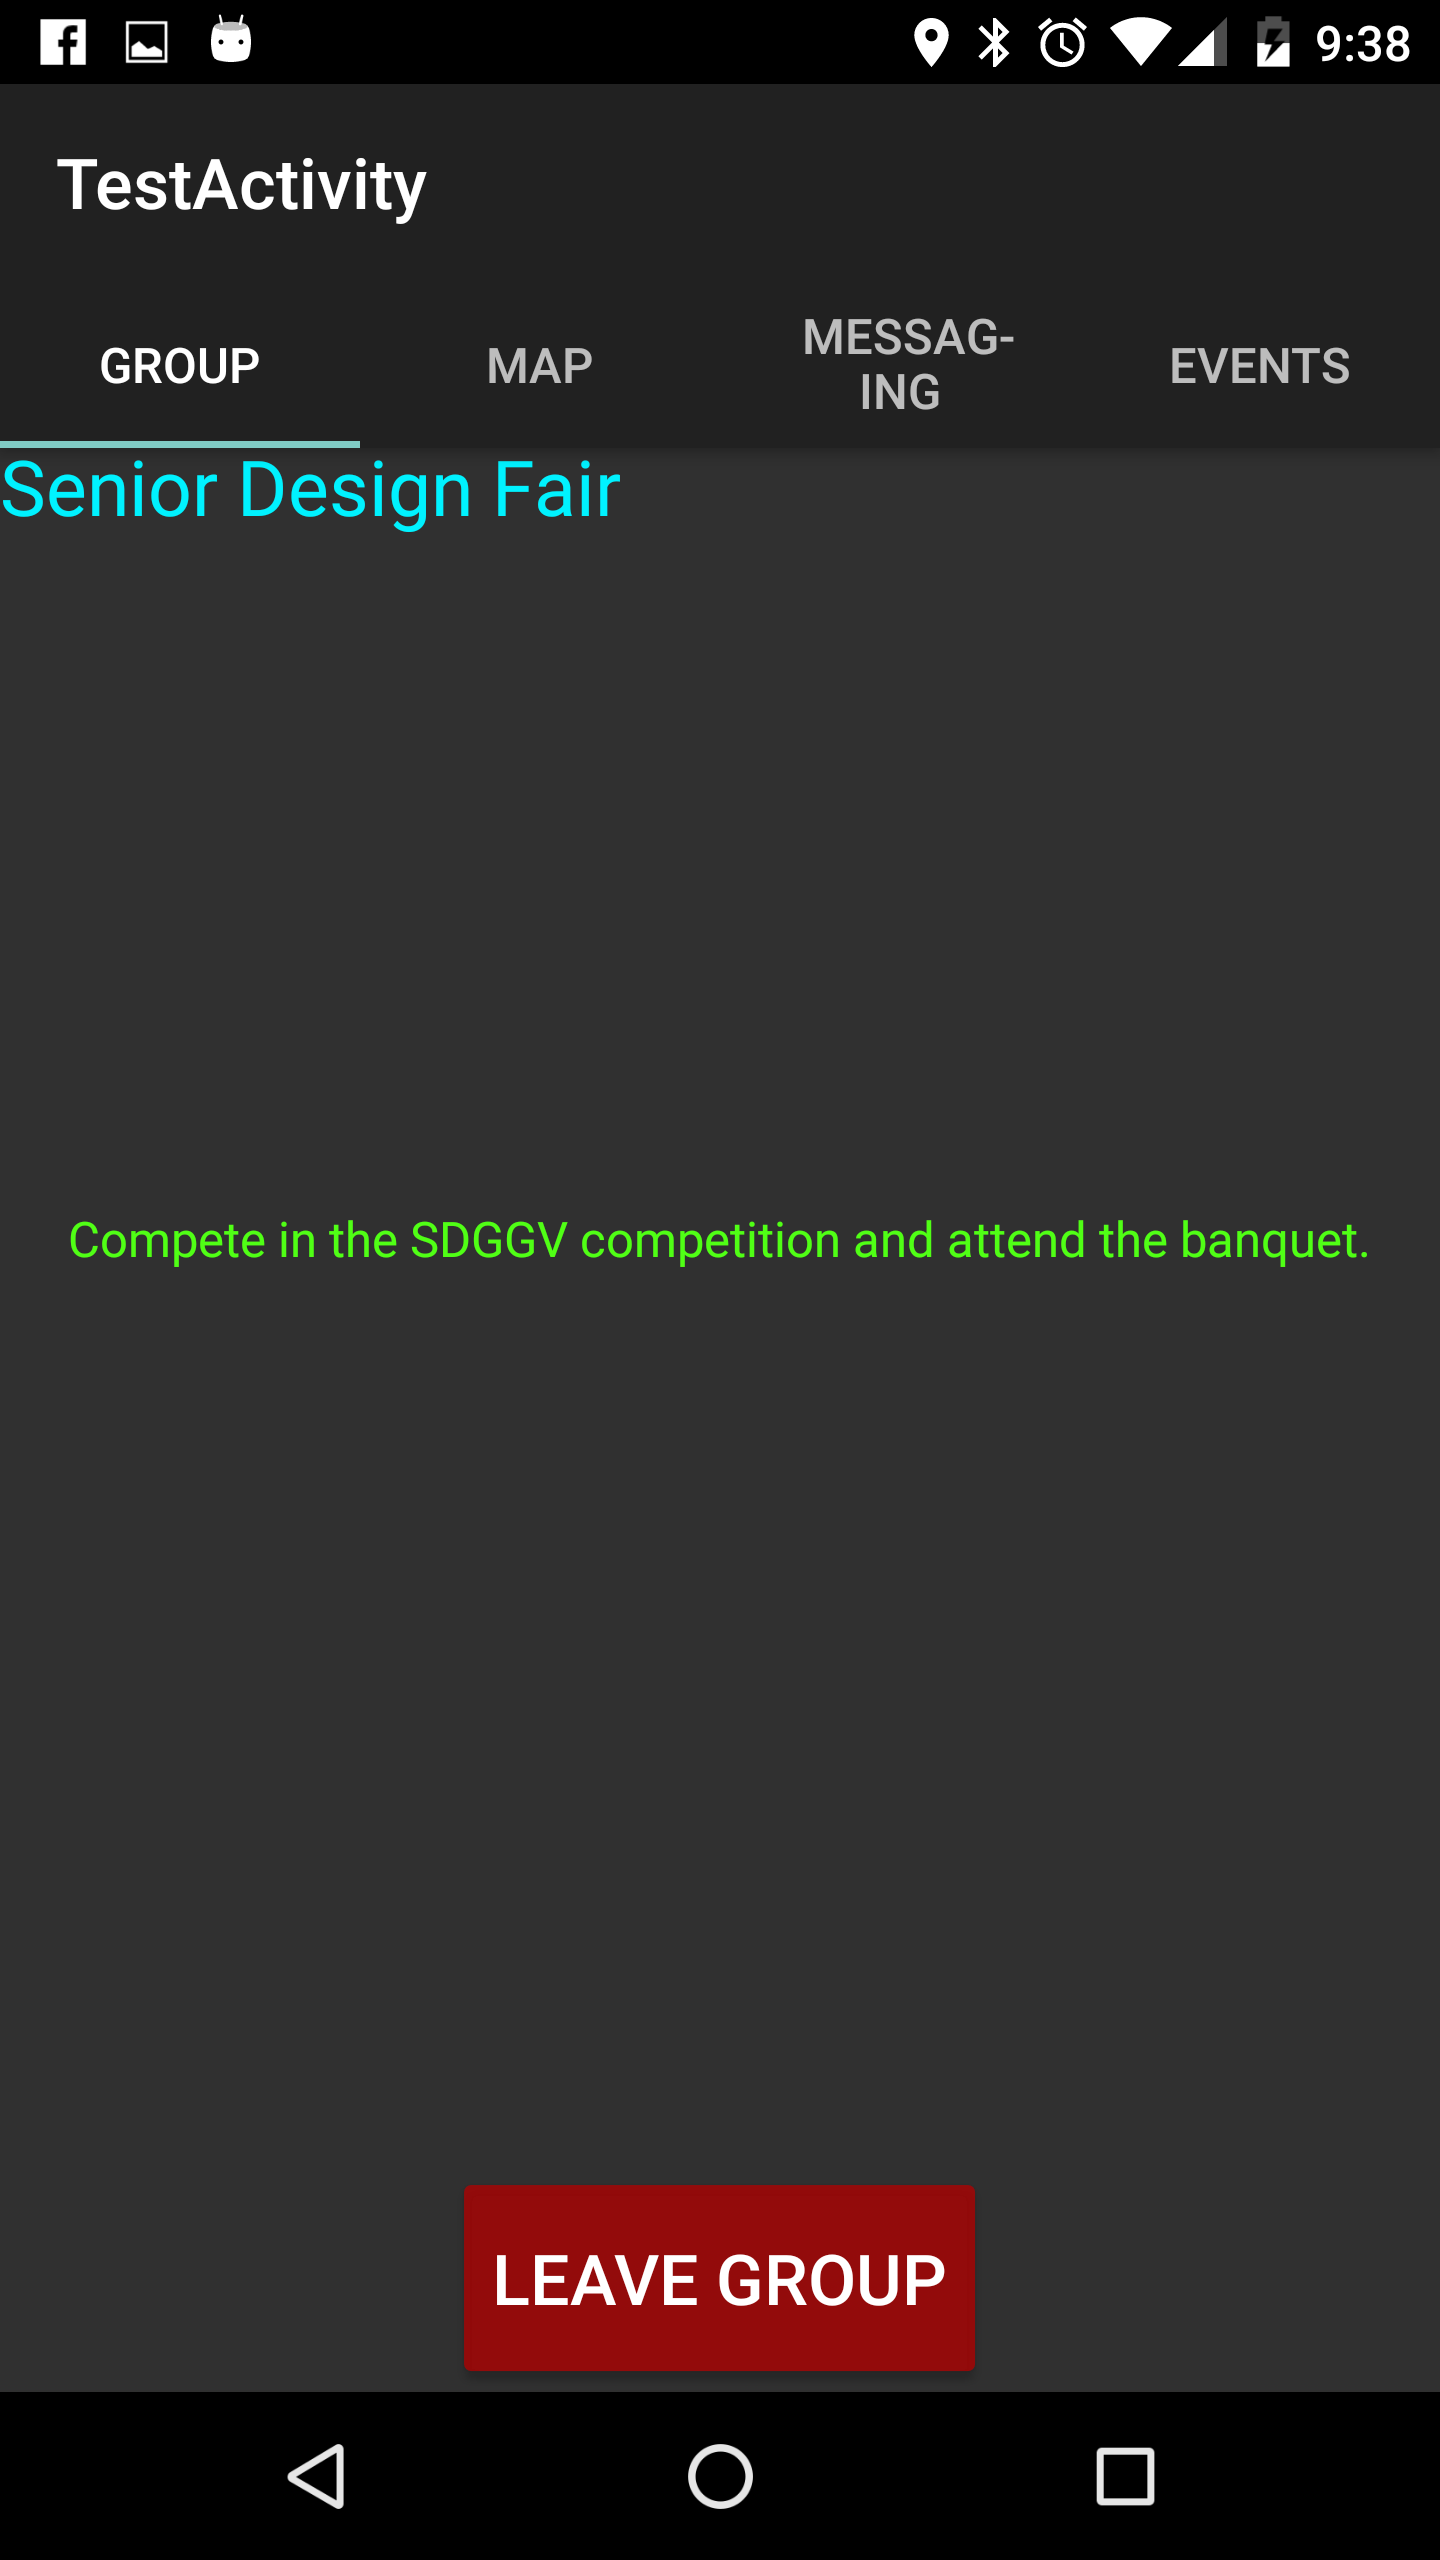
\includegraphics[scale=.1]{Additional/Prototypes/SprintW/info.PNG}}
	\fbox{\includegraphics[scale=.1]{Additional/Prototypes/SprintW/join.PNG}}
	\fbox{\includegraphics[scale=.1]{Additional/Prototypes/SprintW/messaging.PNG}}
	\end{center}
	\caption{Winter Sprint Prototypes. \label{CommFlow}}
	\end{figure}

\subsection{Deliverable}
\begin{itemize}
	\item iOS
	\begin{itemize}
		\item Log-in/Log-out
		\begin{itemize}
			\item Improved Log-in/sign-up screens
			\item Added Log-out feature
		\end{itemize}
		\item Settings
		\begin{itemize}
			\item Implemented settings screen
			\item Nested log-out functionality into settings screen
		\end{itemize}
		\item Groups
		\begin{itemize}
			\item Implemented leaving/Joining a group
			\item Improved basic group operations
			\item Detects if users are in a group
		\end{itemize}
	\end{itemize}
	\item Android
	\begin{itemize}
		\item Log-in
		\begin{itemize}
			\item Automatic log-in on start-up (from data-store)
			\item Log-in to existing account via email address
		\end{itemize}
		\item Settings
		\begin{itemize}
			\item Page layout created and linked from GroupJoin page
			\item Log-out functionality implemented
		\end{itemize}
		\item Groups
		\begin{itemize}
			\item Leave button implemented
			\item Tested adding/removing users from groups
		\end{itemize}
	\end{itemize}
	\item Misc/Transitional
	\begin{itemize}
		\item Further documented Android code to prepare for team merge
		\item Android code review with iOS team, to prepare for team merge
	\end{itemize}
\end{itemize}
\subsection{Backlog}
\begin{itemize}
	\item Android
	\begin{itemize}
		\item Messaging (Sinch API)
		\item GPS Location (back-end models)
		\item Persistent groups through local data-store
	\end{itemize}
	\item iOS
	\begin{itemize}
		\item Messaging (Sinch API)
	\end{itemize}
\end{itemize}
\subsection{Success/Fail}
\begin{itemize}
	\item 
	\begin{itemize}
		\item Messaging wasn't touched
		\item Android is still missing GPS location work
		\item User does not automatically connect to a group if they are in one
	\end{itemize}
	\item Successes
	\begin{itemize}
		\item Android
		\begin{itemize}
			\item Log-in through email
			\item Settings page (layout and implementation)
			\item Local Data-store (individual automatic log-in)
		\end{itemize}
		\item iOS
		\begin{itemize}
			\item Log-in/Log-out
			\item Settings page (layout and implementation)
			\item Group functionality written
		\end{itemize}
	\end{itemize}
\end{itemize}

\section{Sprint 4 Prototype}

	\begin{figure}[tbh]
	\begin{center}
	\fbox{\includegraphics[scale=.1]{Additional/Prototypes/Sprint4/join.PNG}}
	\fbox{\includegraphics[scale=.1]{Additional/Prototypes/Sprint4/messaging.PNG}}
	\end{center}
	\caption{Sprint 4 Prototypes. \label{CommFlow}}
	\end{figure}

\subsection{Deliverable}
\begin{itemize}
	\item Android
	\begin{itemize}
		\item Group Messaging
		\begin{itemize}
			\item Created a Layout
			\item Used Sinch code to create a service
			\item Implemented group messaging
			\item Group messaging is working with no known bugs
			\end{itemize}
		\item Location
		\begin{itemize}
			\item Page layout created and linked from GroupJoin page
			\item MapFragment has buttons for homing and syncing group locations
			\item Retrieving the user's location on instantiation of the MapFragment
			\item User and group locations implemented
		\end{itemize}
		\item Group update service
		\begin{itemize}
			\item Checks for updates in near real-time
			\item Updates group settings when changed
			\item Updates group members if someone leaves or joins
		\end{itemize}
	\end{itemize}
	\item Server (cloud code)
	\begin{itemize}
		\item Functional Group update indicator
		\item Returning group update information
		\item Join group function (created but not functioning)
		\item Leave group function (created but not functioning)
		\item Check for Existing Email
	\end{itemize}	
	\item Misc/Transitional
	\begin{itemize}
		\item Business Plan filled out, also a version tailored towards the Governor's Giant Vision contest (converted to latex)
		\item Documentation done inside and outside of the source code files
	\end{itemize}
\end{itemize}
\subsection{Backlog}
\begin{itemize}
	\item Android
	\begin{itemize}
		\item Begin implementing Sinch
		\item Create location and messaging views and managers
		\item Design models and manager classes for messaging and location
		\item Broadcast/receive messages to/from all members in a group
		\item Create a layout for messaging
		\item Create a MapFragment to display a map
		\item Create buttons over top the MapFragment to correspond to syncing and homing locations
		\item Retrieve locations of group members, place their locations on the map via pins
		\item Update group settings and data when changed
		\item Update Group members if someone leaves or joins a group
		\item Create Group messaging unit tests
		\item Create GPS Location unit tests
	\end{itemize}
	\item Cloud Code
	\begin{itemize}
		\item Start Group data parsing
		\item Handled Leaving and joining groups
		\item Validated Checking existing email upon log-in
		\item Return group information upon changes
		\item Create Functional Group update indicator complete
		\item Implement Basic group functionality fully (log-in/log-out, join/leave groups, update on change)
	\end{itemize}
	\item Turn in business plan to Governor's Giant Vision
\end{itemize}
\subsection{Success/Fail}
\begin{itemize}
	\item Failures
	\begin{itemize}
		\item Android
		\begin{itemize}
			\item Did not create group messaging unit test
			\item Did not create GPS location unit test
		\end{itemize}
		\item Cloud Code
		\begin{itemize}
			\item Did not implement group function tests
			\item Did not complete Join and Leave functions
		\end{itemize}
	\end{itemize}
	\item Success
	\begin{itemize}
		\item Completed basic messaging
		\item Completed basic GPS functionality
		\item Created an update service that is the backbone of the app
		\item Progress made on safe group operations
		\item Passed into the Governor's Giant Vision contest finals
	\end{itemize}
\end{itemize}

\section{Sprint 5 Prototype}

	\begin{figure}[tbh]
	\begin{center}
	\fbox{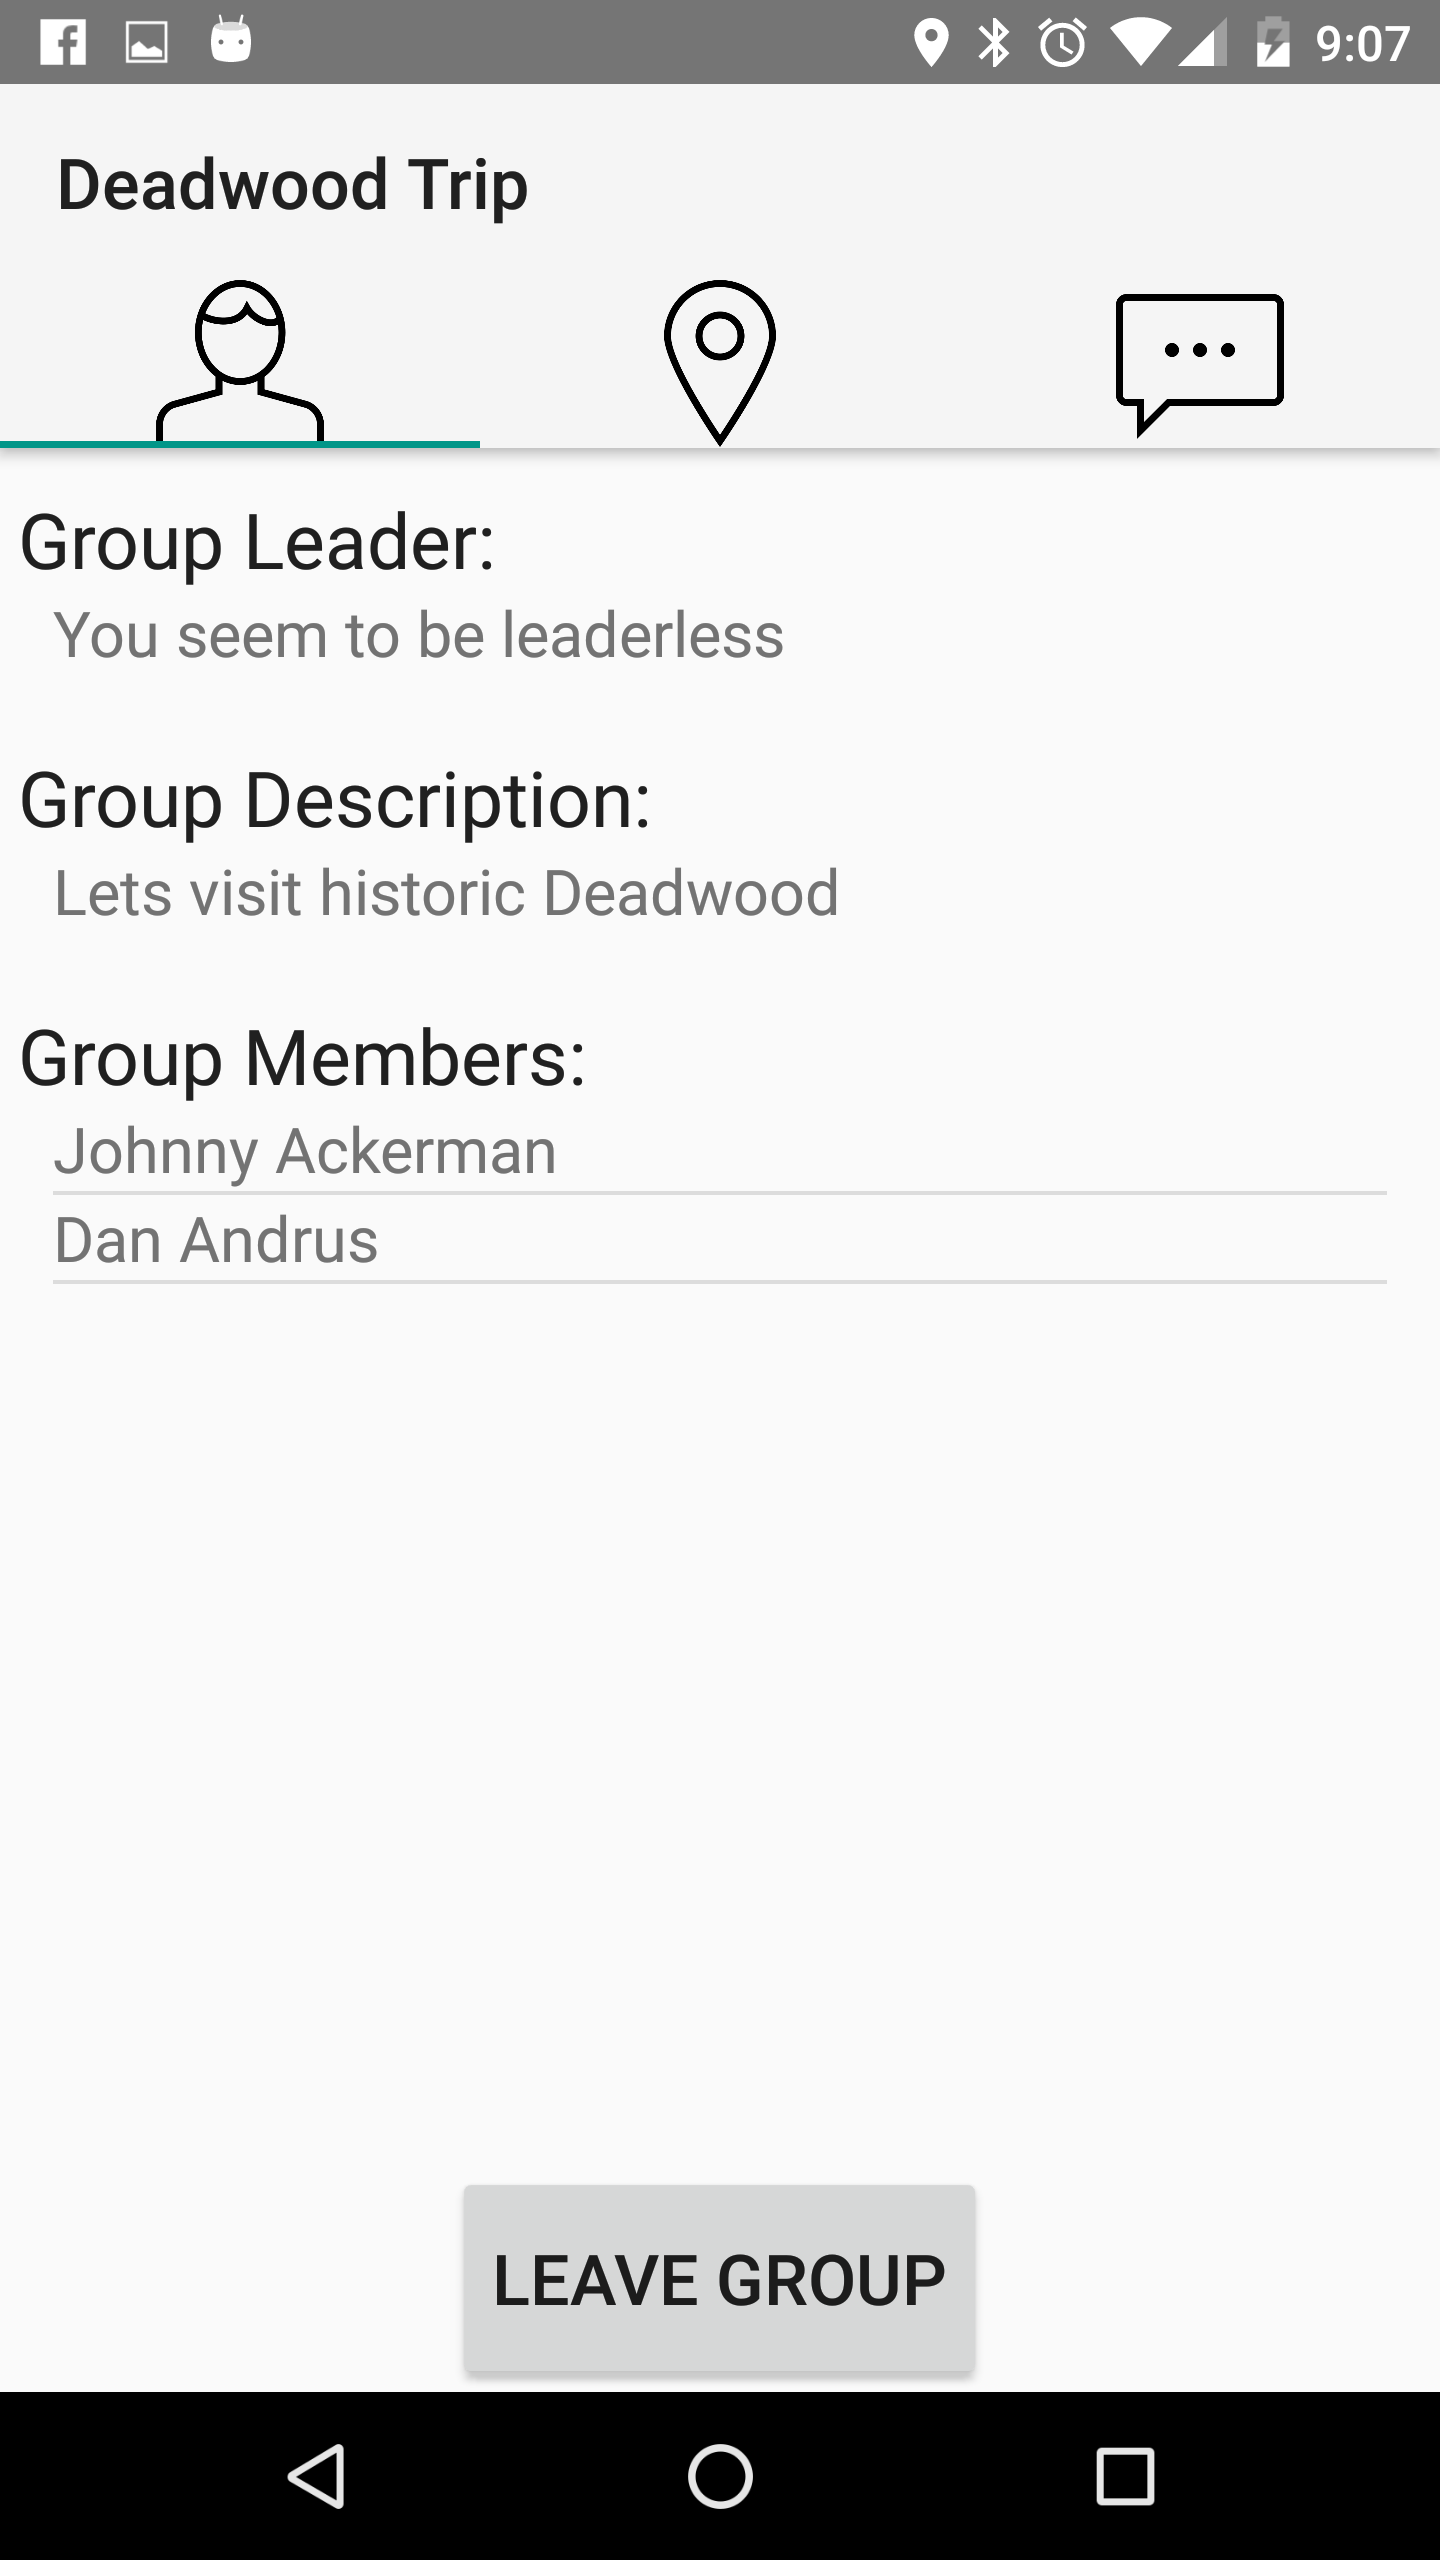
\includegraphics[scale=.1]{Additional/Prototypes/Sprint5/groupInfo.PNG}}
	\fbox{\includegraphics[scale=.1]{Additional/Prototypes/Sprint5/leaving.PNG}}
	\fbox{\includegraphics[scale=.1]{Additional/Prototypes/Sprint5/login.PNG}}
	\fbox{\includegraphics[scale=.1]{Additional/Prototypes/Sprint5/map.PNG}}
	\fbox{\includegraphics[scale=.1]{Additional/Prototypes/Sprint5/messaging.PNG}}
	\end{center}
	\caption{Sprint 5 Prototypes. \label{CommFlow}}
	\end{figure}

\subsection{Deliverable}
\begin{itemize}
	\item Android
	\begin{itemize}
		\item Group Messaging
		\begin{itemize}
			\item Discovered and removed a bug
		\end{itemize}
	\item Location
	\begin{itemize}
		\item Moved remote functionality to model manager
		\item Updated location model to reflect changes
		\item Caching objects
	\end{itemize}
		\item App Appearance
		\begin{itemize}
			\item Reformatted the entire theme of the app (all pages are based of the same theme now - no more custom themes per page)
			\item Added a tool bar to the group join page/ removed settings button (now in tool bar)
			\item Group Information Page
			\begin{itemize}
				\item Added a group leader display
				\item Added padding to appearance of display and modified text sizes
				\item Displays all group members
				\item Displays Dialog box if user attempts to leave the group
			\end{itemize}
		\end{itemize}
	\end{itemize}
	\item Server (cloud code)
	\begin{itemize}
		\item Join function
		\item Leave function
	\end{itemize}
	\item Misc/Transitional
	\begin{itemize}
		\item Business Plan revised and submitted to The Governor's Giant Vision Competition
		\item Finalist for The Governor's Giant Vision Competition
		\item Some of the overall Senior Design Doc has been touched up
	\end{itemize}
\end{itemize}
\subsection{Backlog}
\begin{itemize}
	\item Senior Design Doc
	\begin{itemize}
		\item Do a general revision of the doc
	\end{itemize}
	\begin{itemize}
		\item Business Plan
		\begin{itemize}
			\item Finish business plan for 2016 Governor's Giant Vision Competition
		\end{itemize}
	\end{itemize}
	\item Android
	\begin{itemize}
		\item Model Caching/ Uniformity
		\item Clean up appearance
		\item Clean up the appearance of the app
		\item Display Group Members on group info page
		\item Safe group operations(leaving/joining group)
		\item Loading animations on homing and syncing
		\item Integration Testing
		\item Start Alpha Testing
	\end{itemize}
	\item Cloud code
	\begin{itemize}
		\item Safe group operations(leaving/joining group)
		\item test join and leave functionality
	\end{itemize}
\end{itemize}
\subsection{Success/Fail}
\begin{itemize}
	\item Failures
	\begin{itemize}
		\item Android
		\begin{itemize}
			\item Messaging still needs an appearance update for usability
		\end{itemize}
		\begin{itemize}
			\item Cloud Code
			\begin{itemize}	
				\item Needs more testing on group functions
				\item Completing join and leave functions
			\end{itemize}
		\end{itemize}
	\end{itemize}
	\item Successes
	\begin{itemize}
		\item Added safe group operations though cloud code
		\item Reformatted the theme of the app
		\item Added tool bar to tab section of groups
		\item Finalist for The Governor's Giant Vision Competition
		\item Fixed a few bugs in the location code
	\end{itemize}
\end{itemize}


\section{Sprint 6 Prototype}

	\begin{figure}[tbh]
	\begin{center}
	\fbox{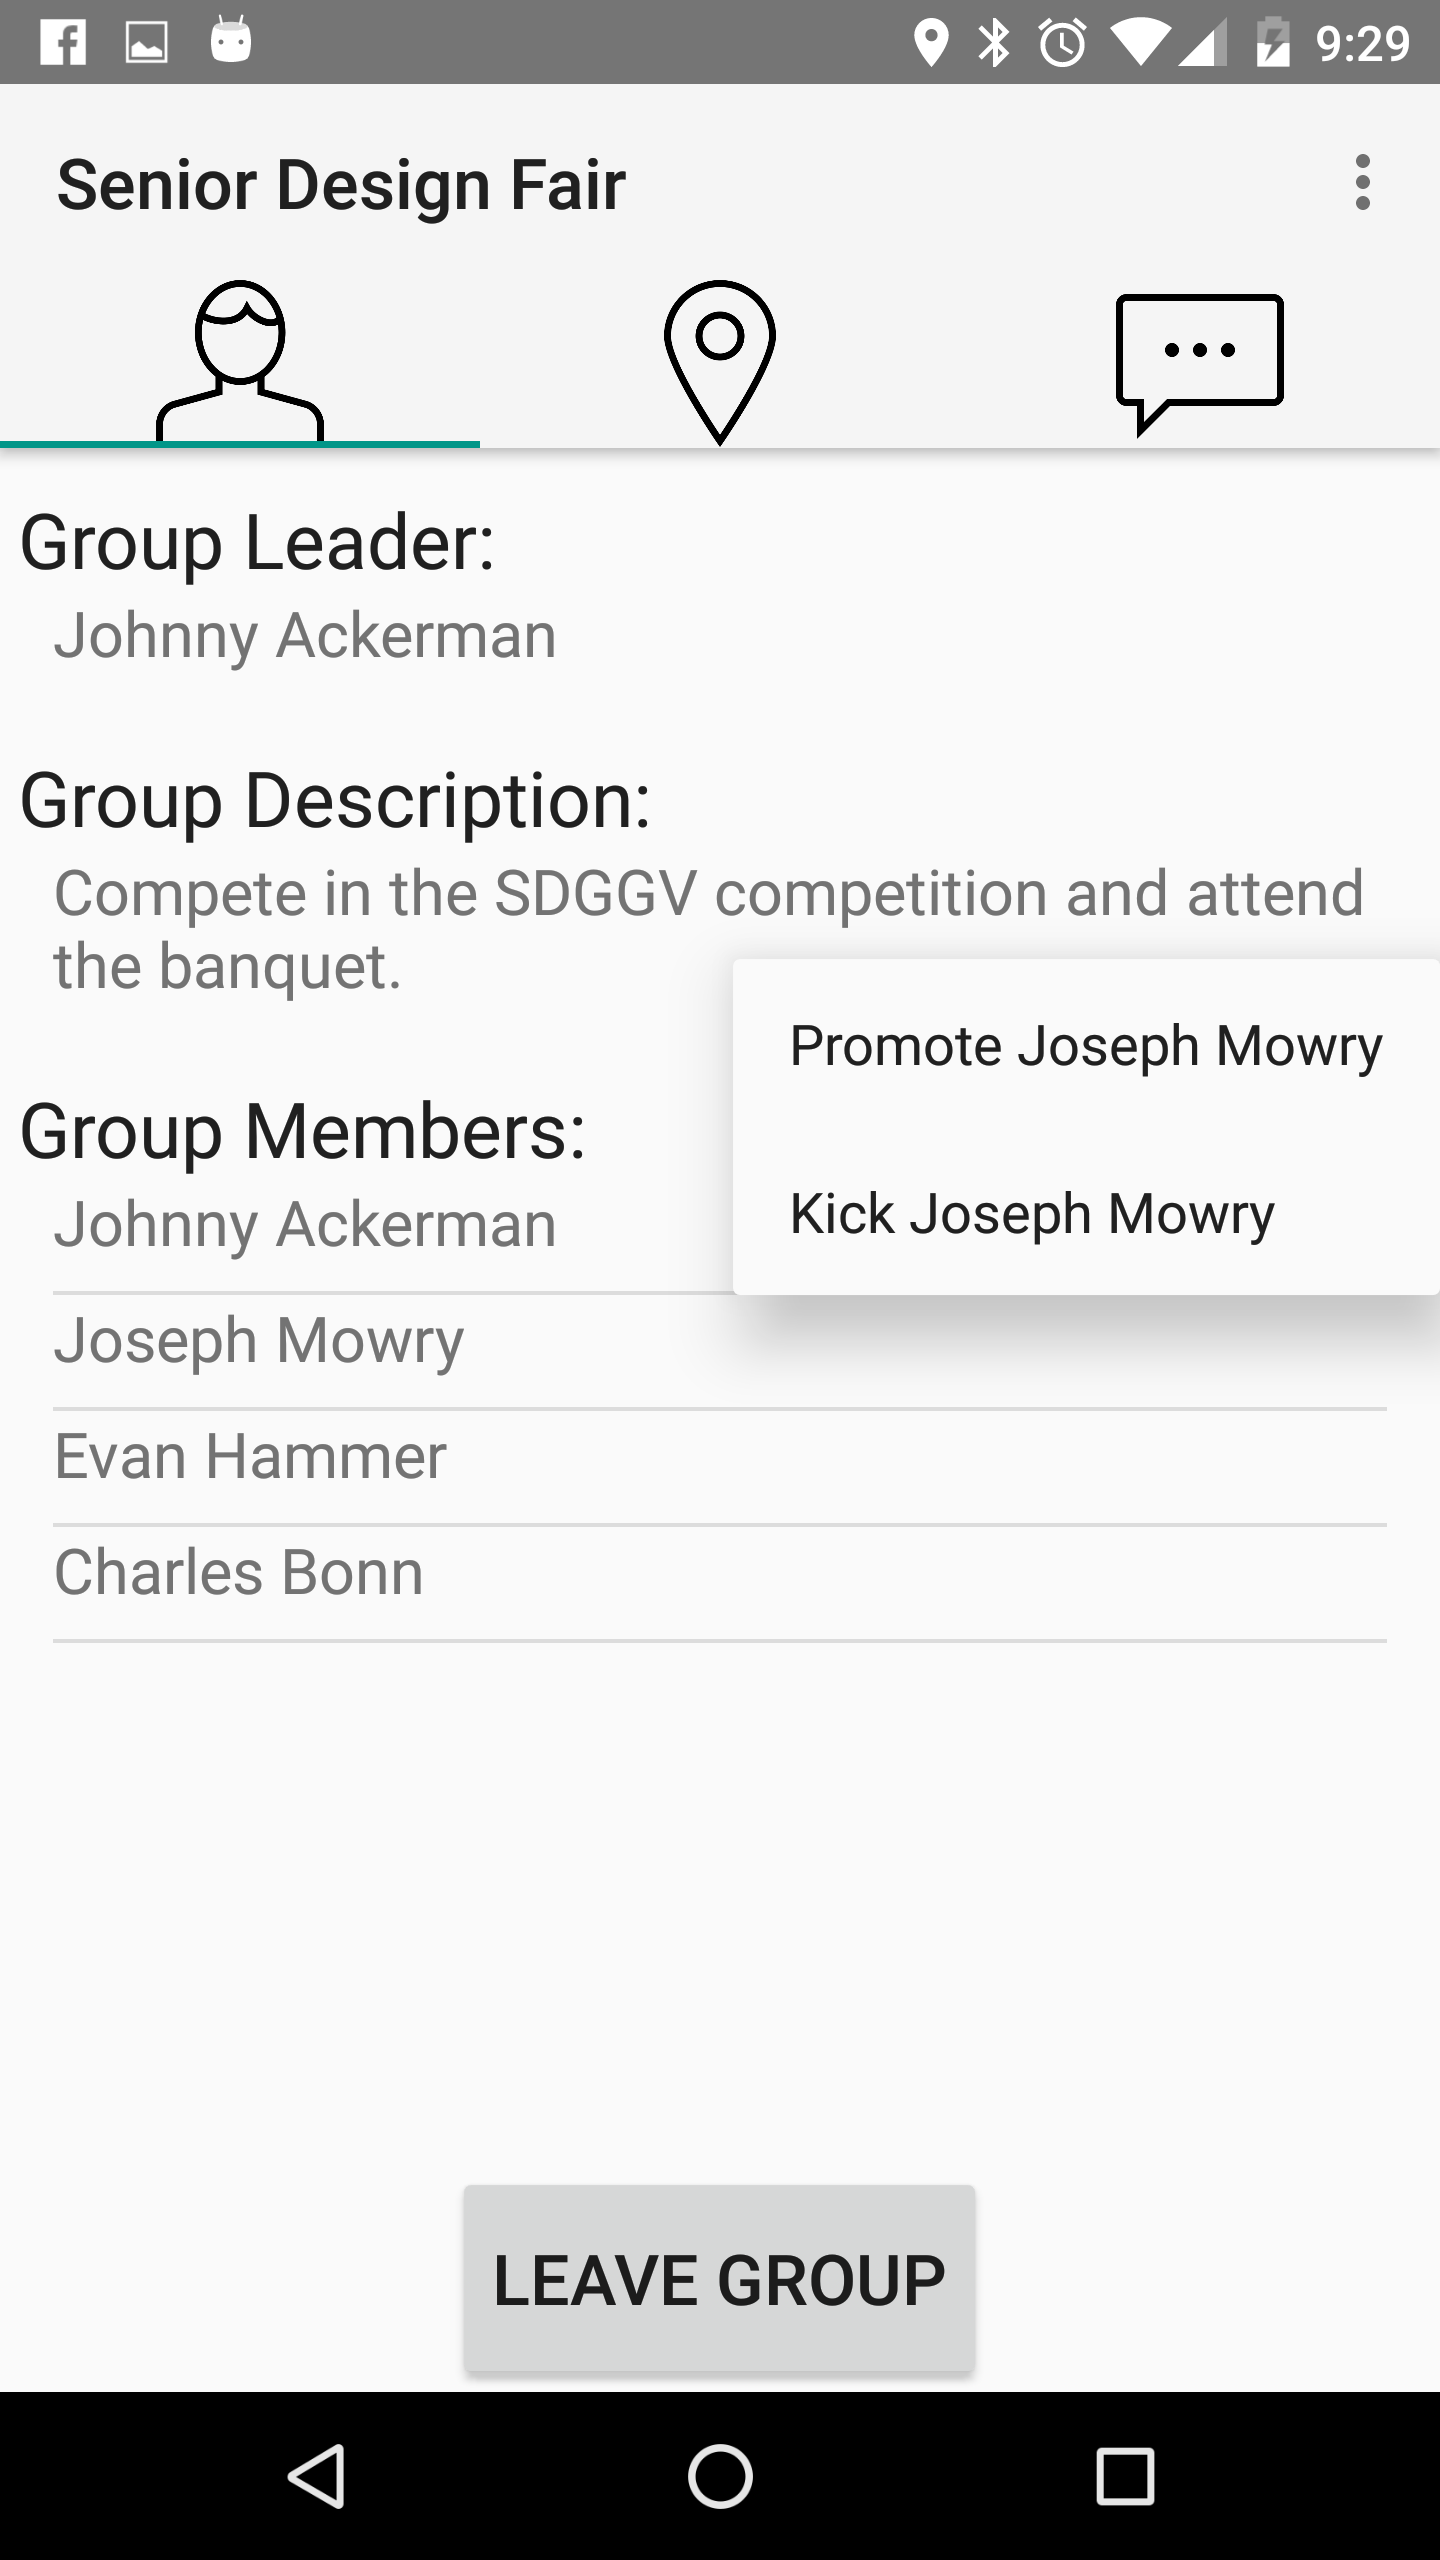
\includegraphics[scale=.1]{Additional/Prototypes/Sprint6/commands.PNG}}
	\fbox{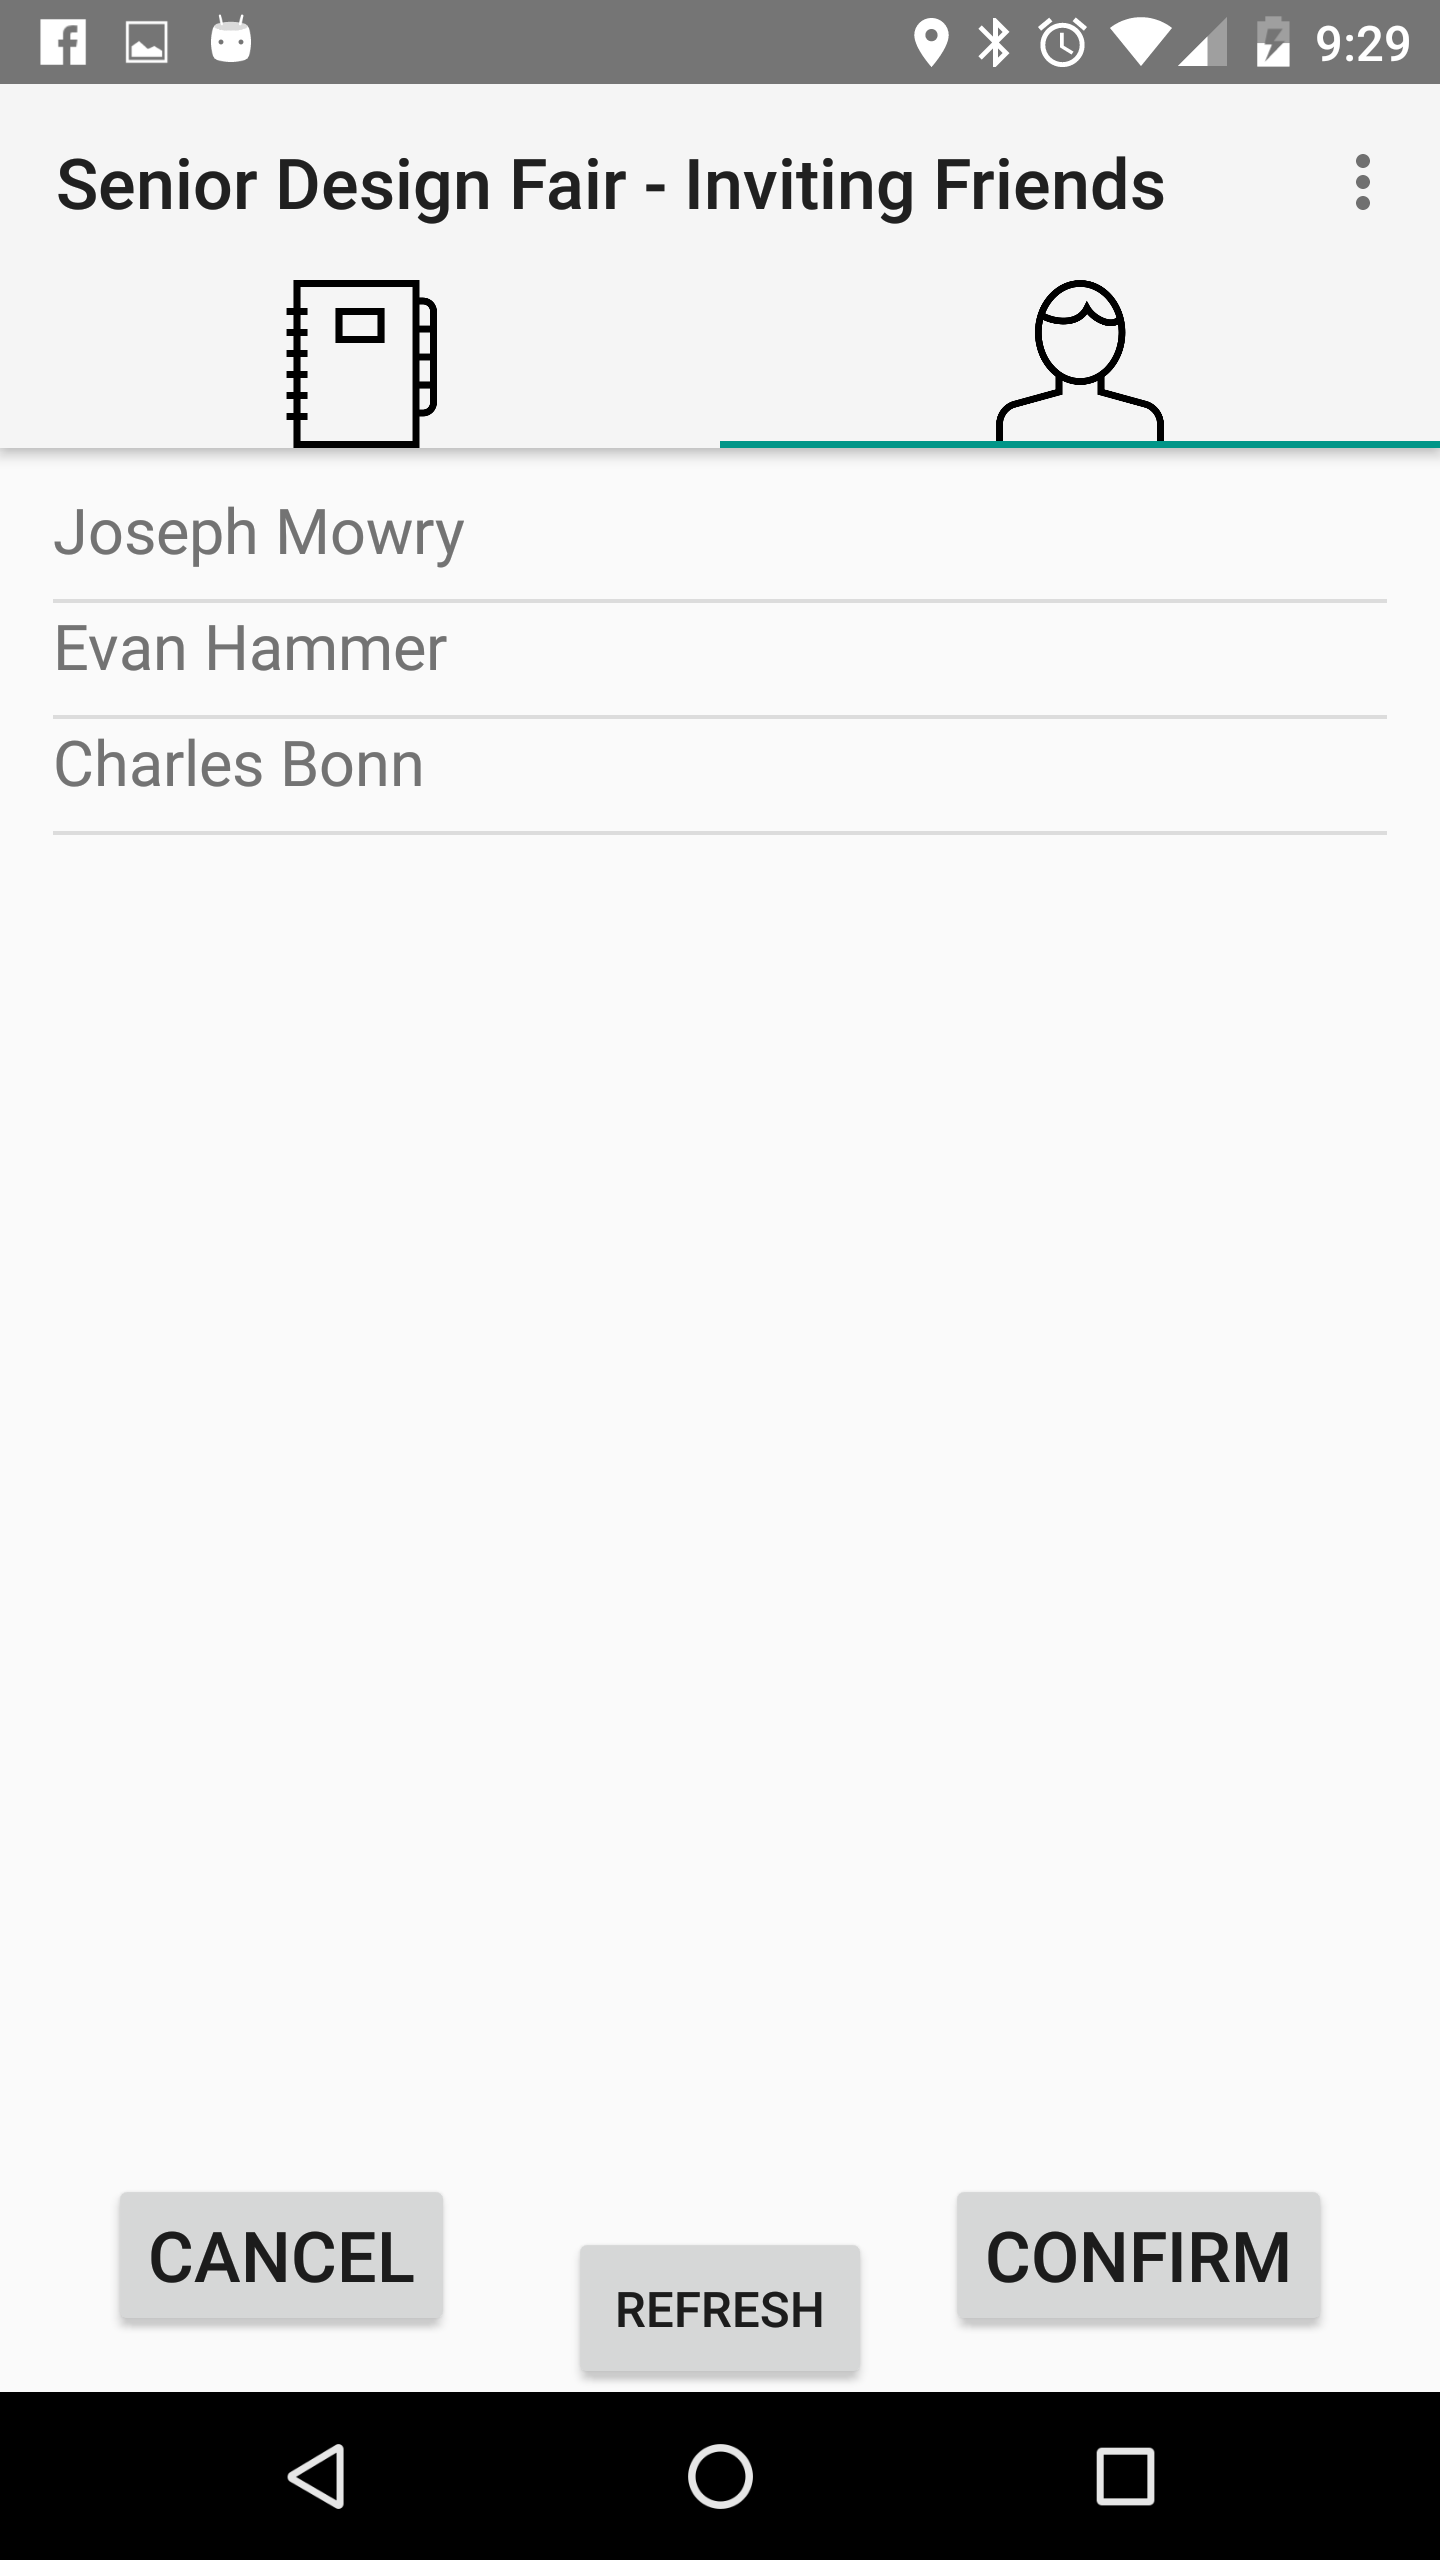
\includegraphics[scale=.1]{Additional/Prototypes/Sprint6/confirm.PNG}}
	\fbox{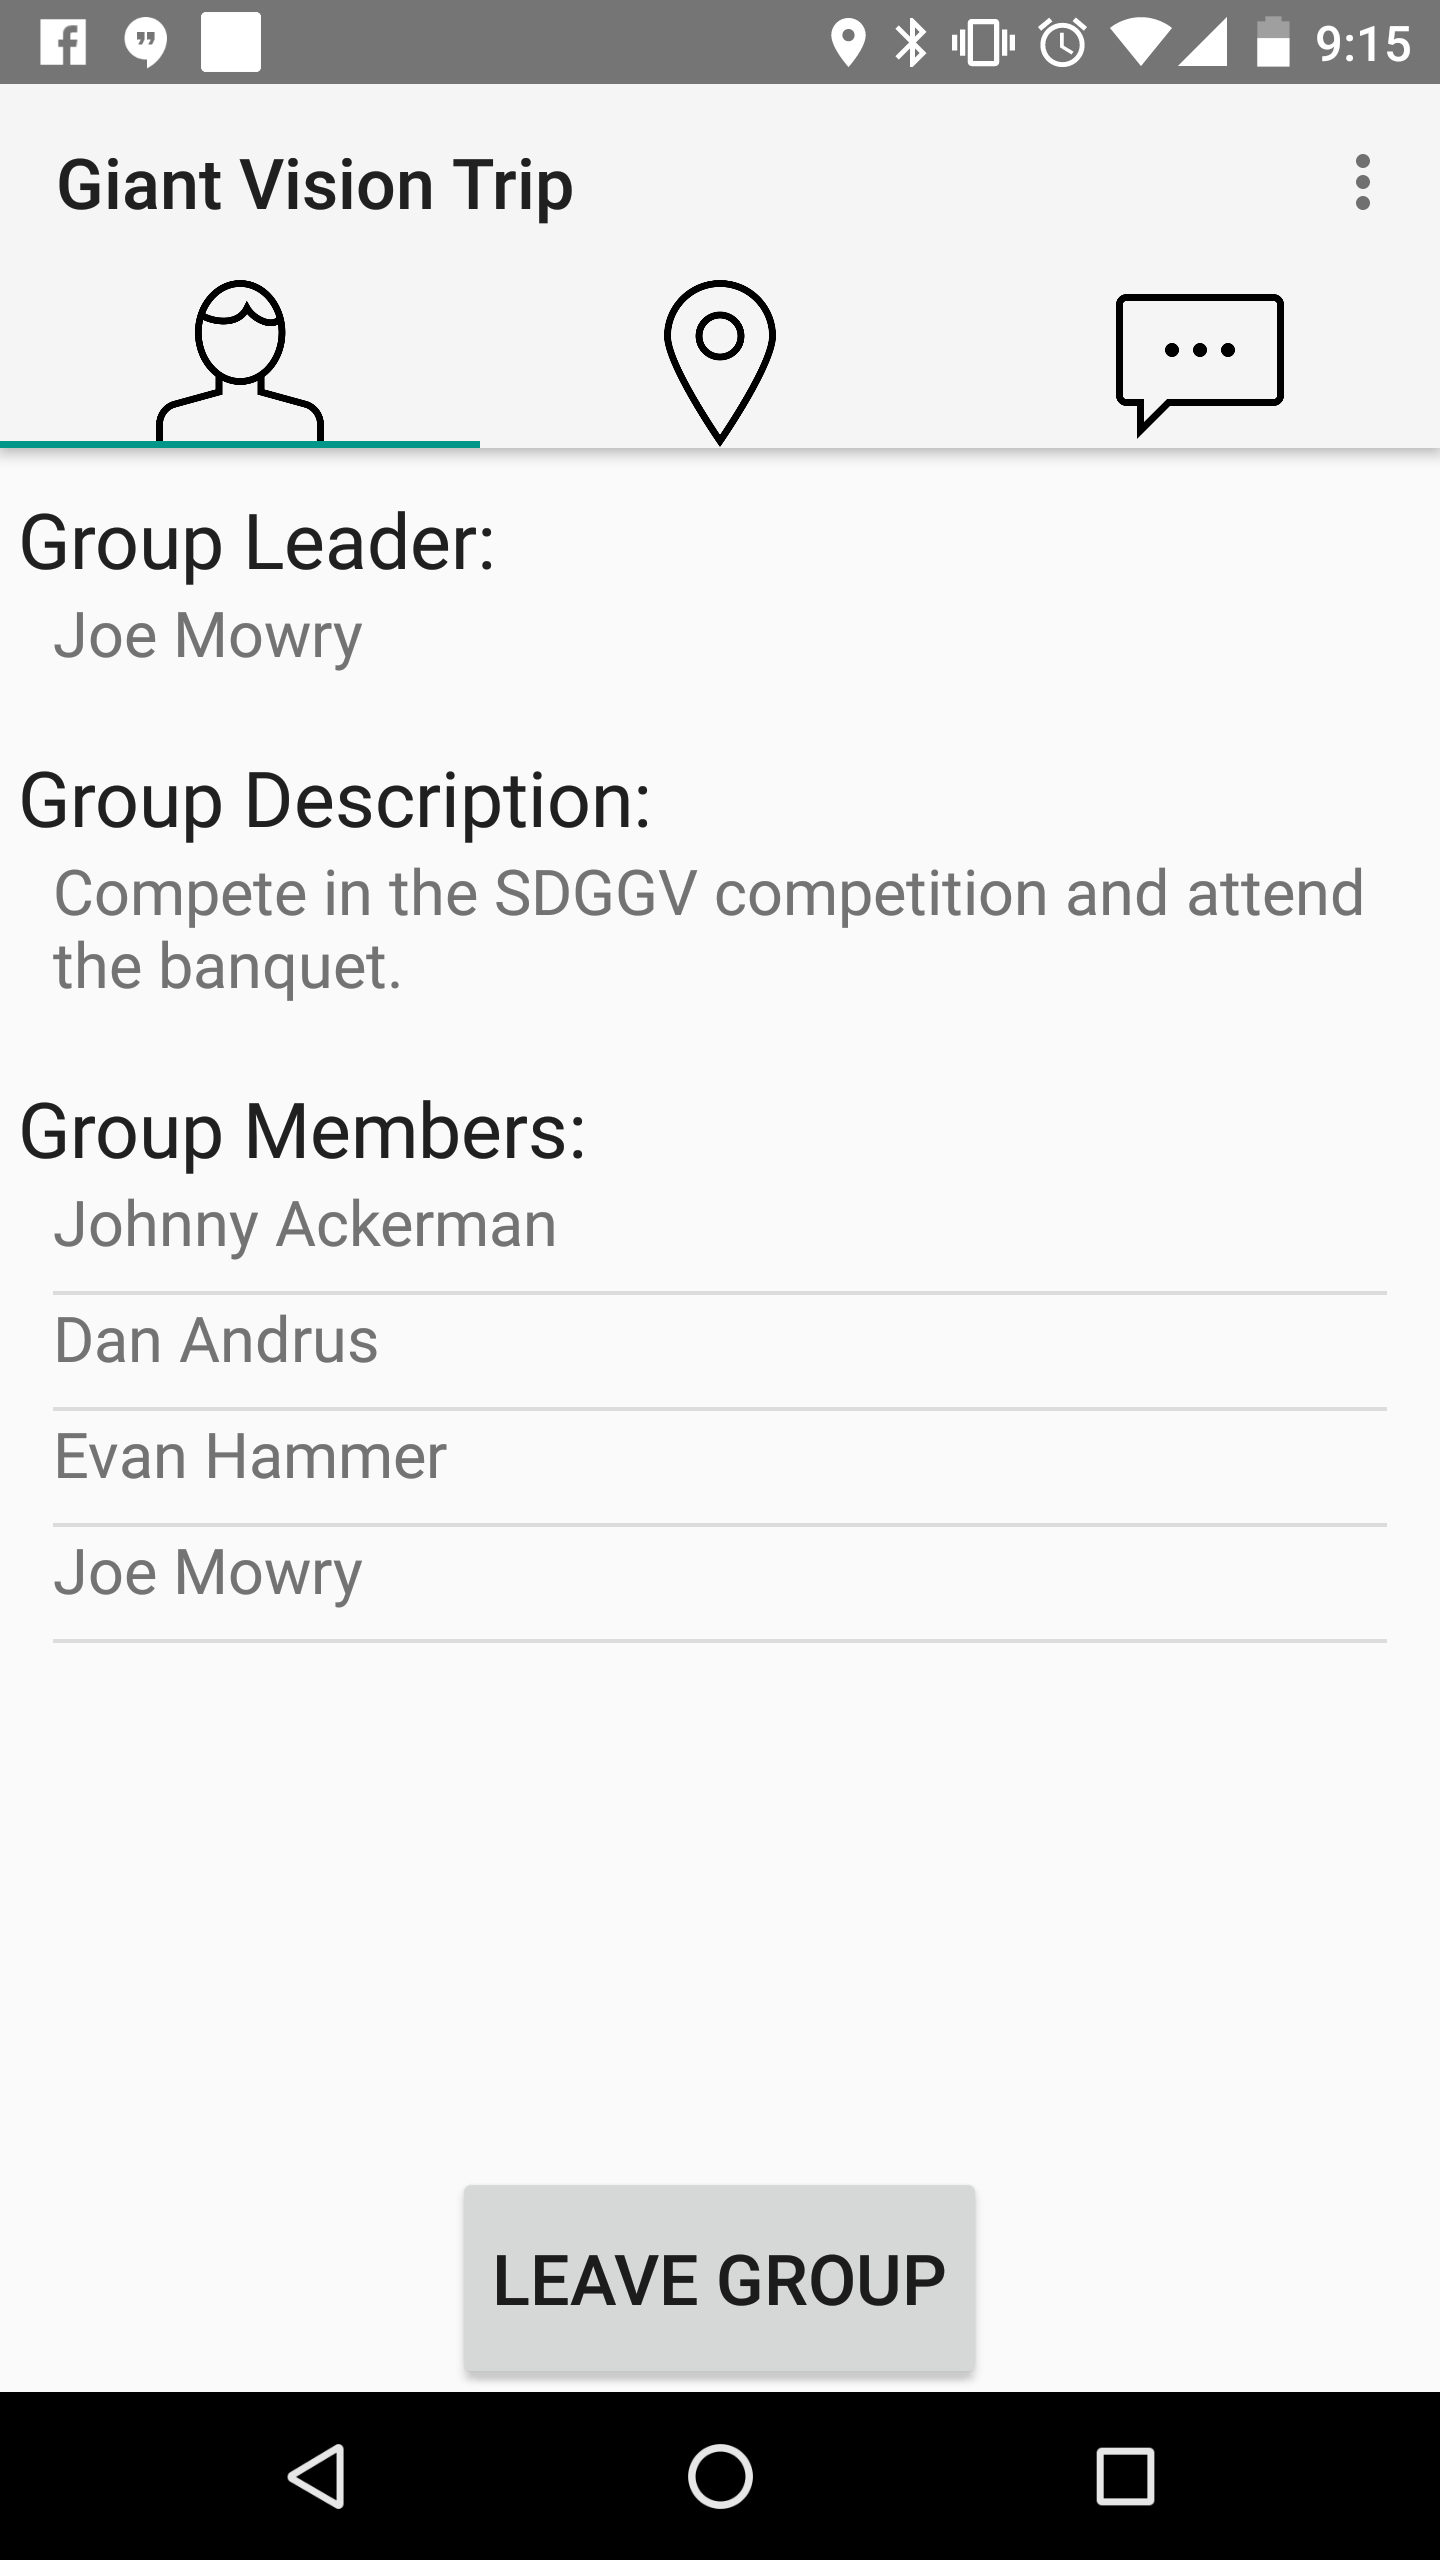
\includegraphics[scale=.1]{Additional/Prototypes/Sprint6/groupActivity.PNG}}
	\fbox{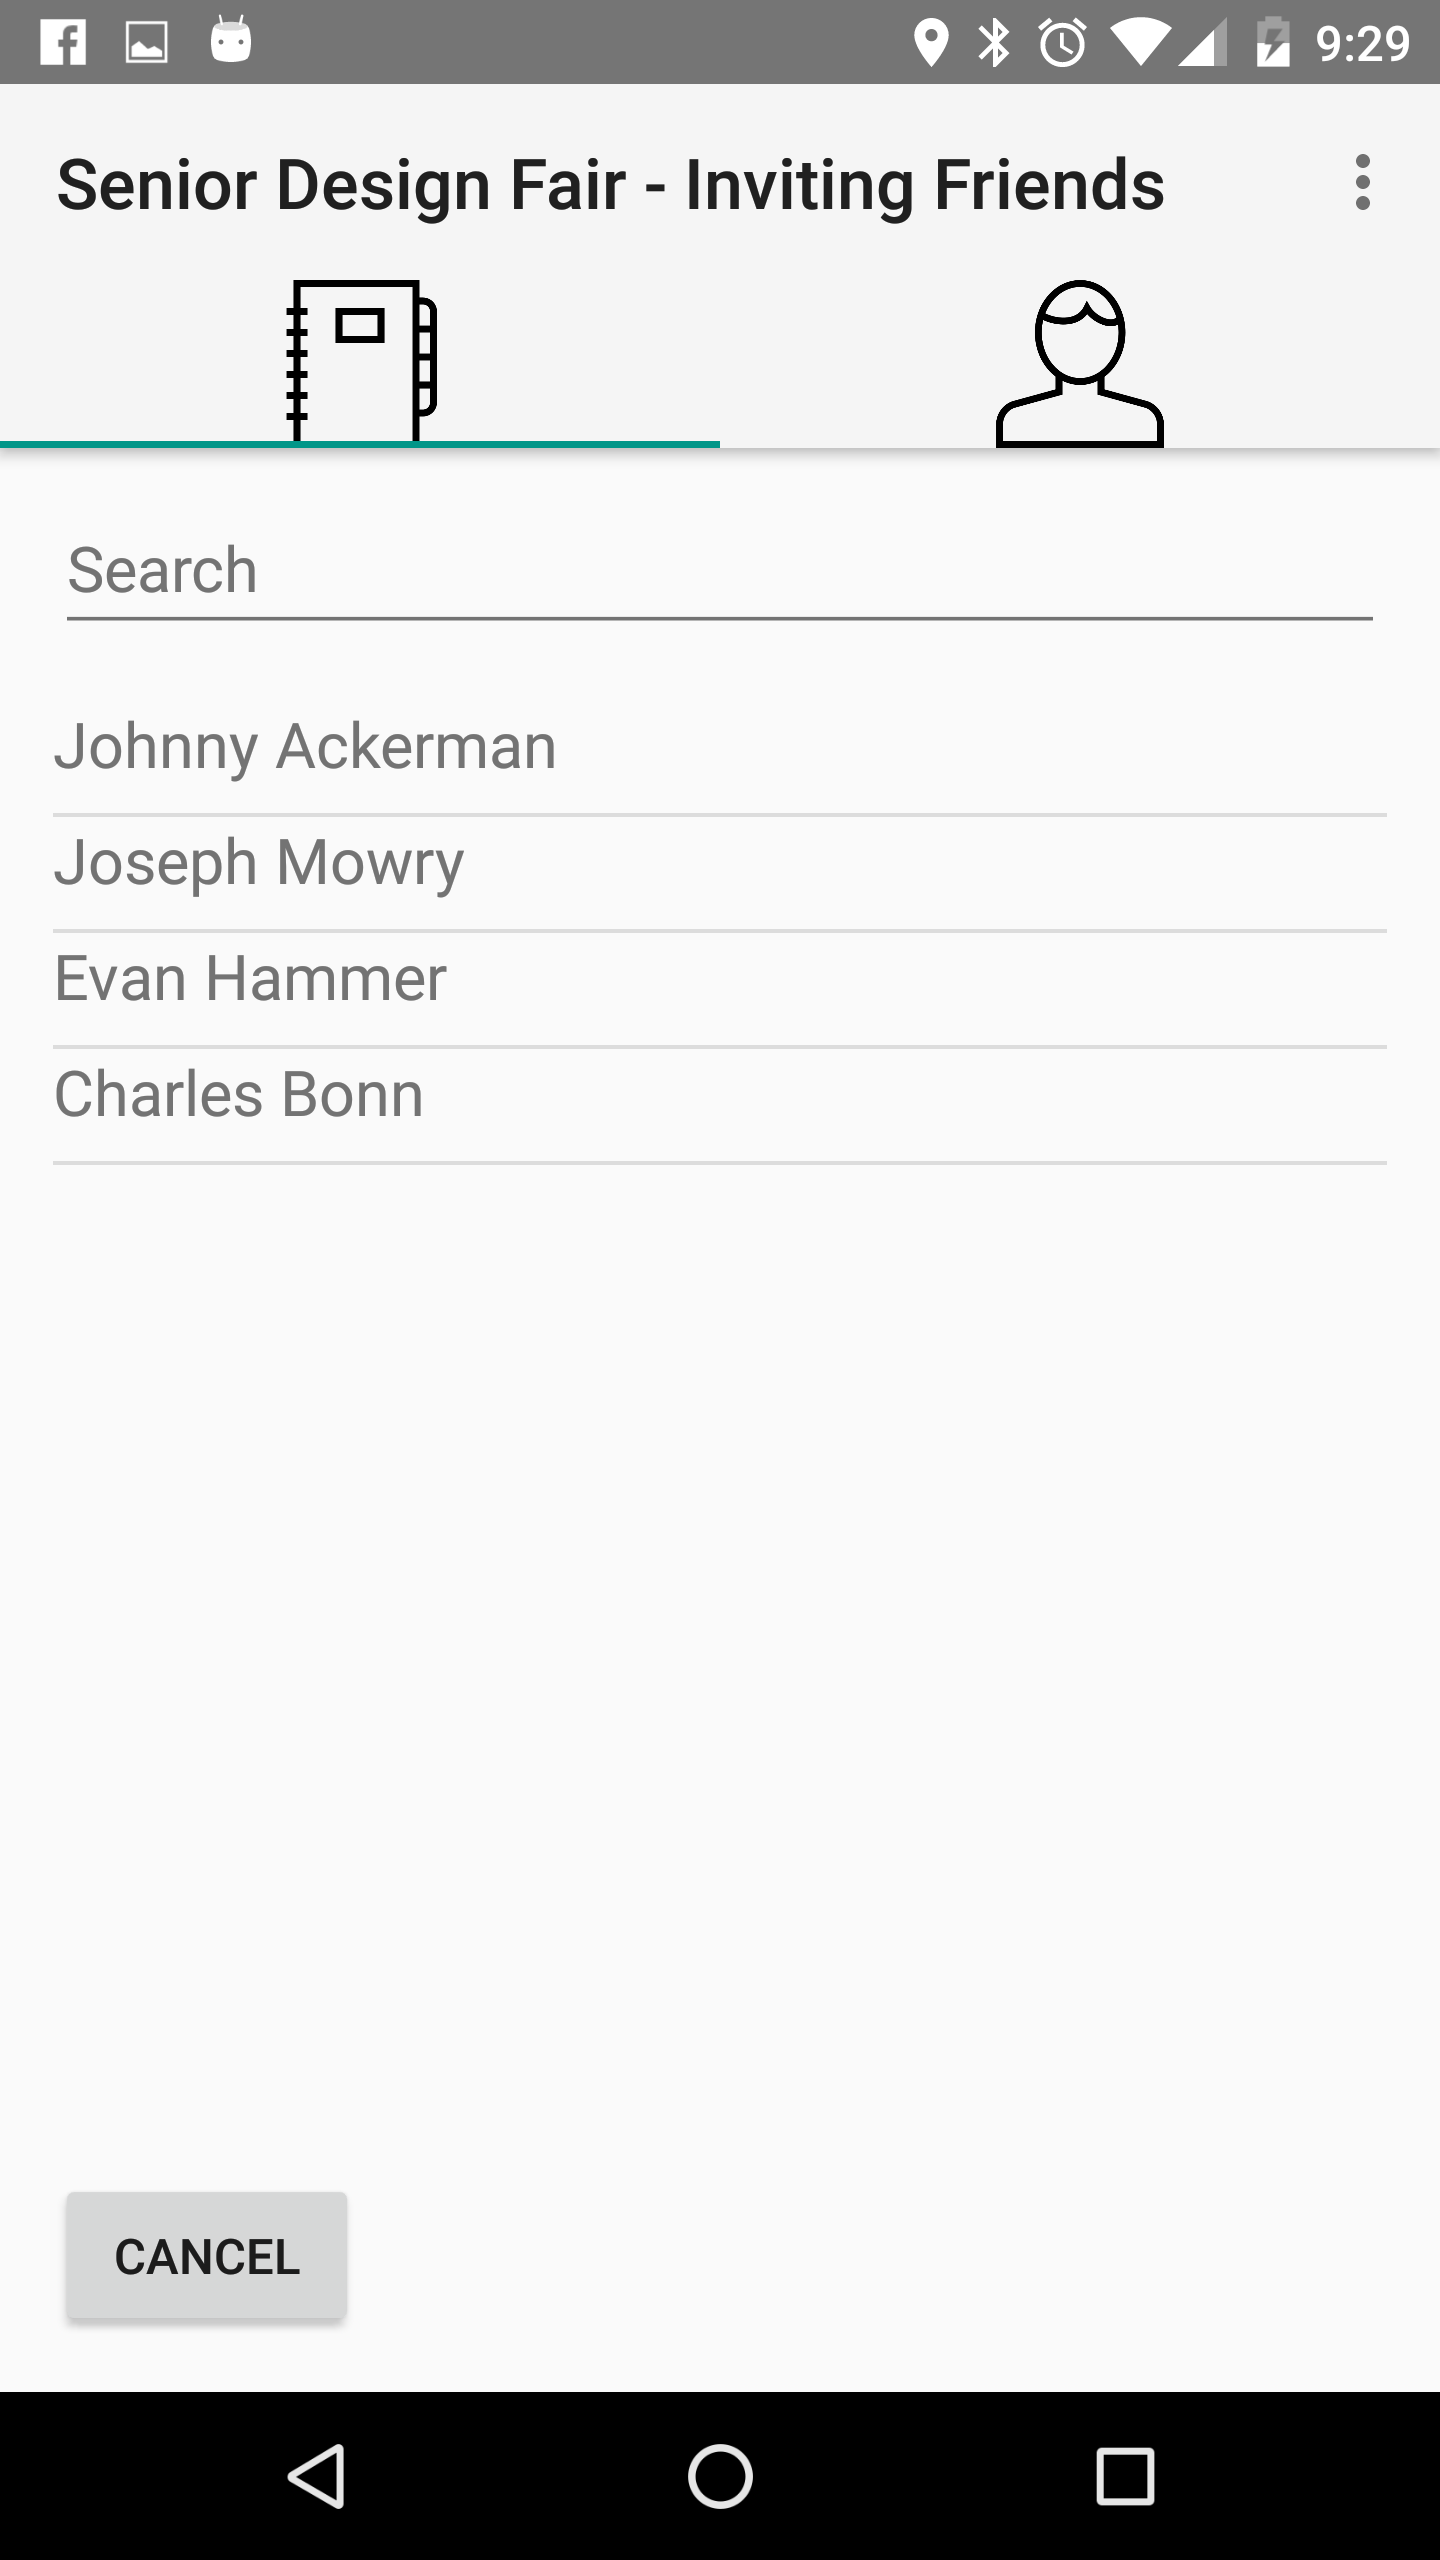
\includegraphics[scale=.1]{Additional/Prototypes/Sprint6/invite.PNG}}
	\fbox{\includegraphics[scale=.1]{Additional/Prototypes/Sprint6/leaving.PNG}}
	\fbox{\includegraphics[scale=.1]{Additional/Prototypes/Sprint6/logIn.PNG}}
	\fbox{\includegraphics[scale=.1]{Additional/Prototypes/Sprint6/map.PNG}}
	\fbox{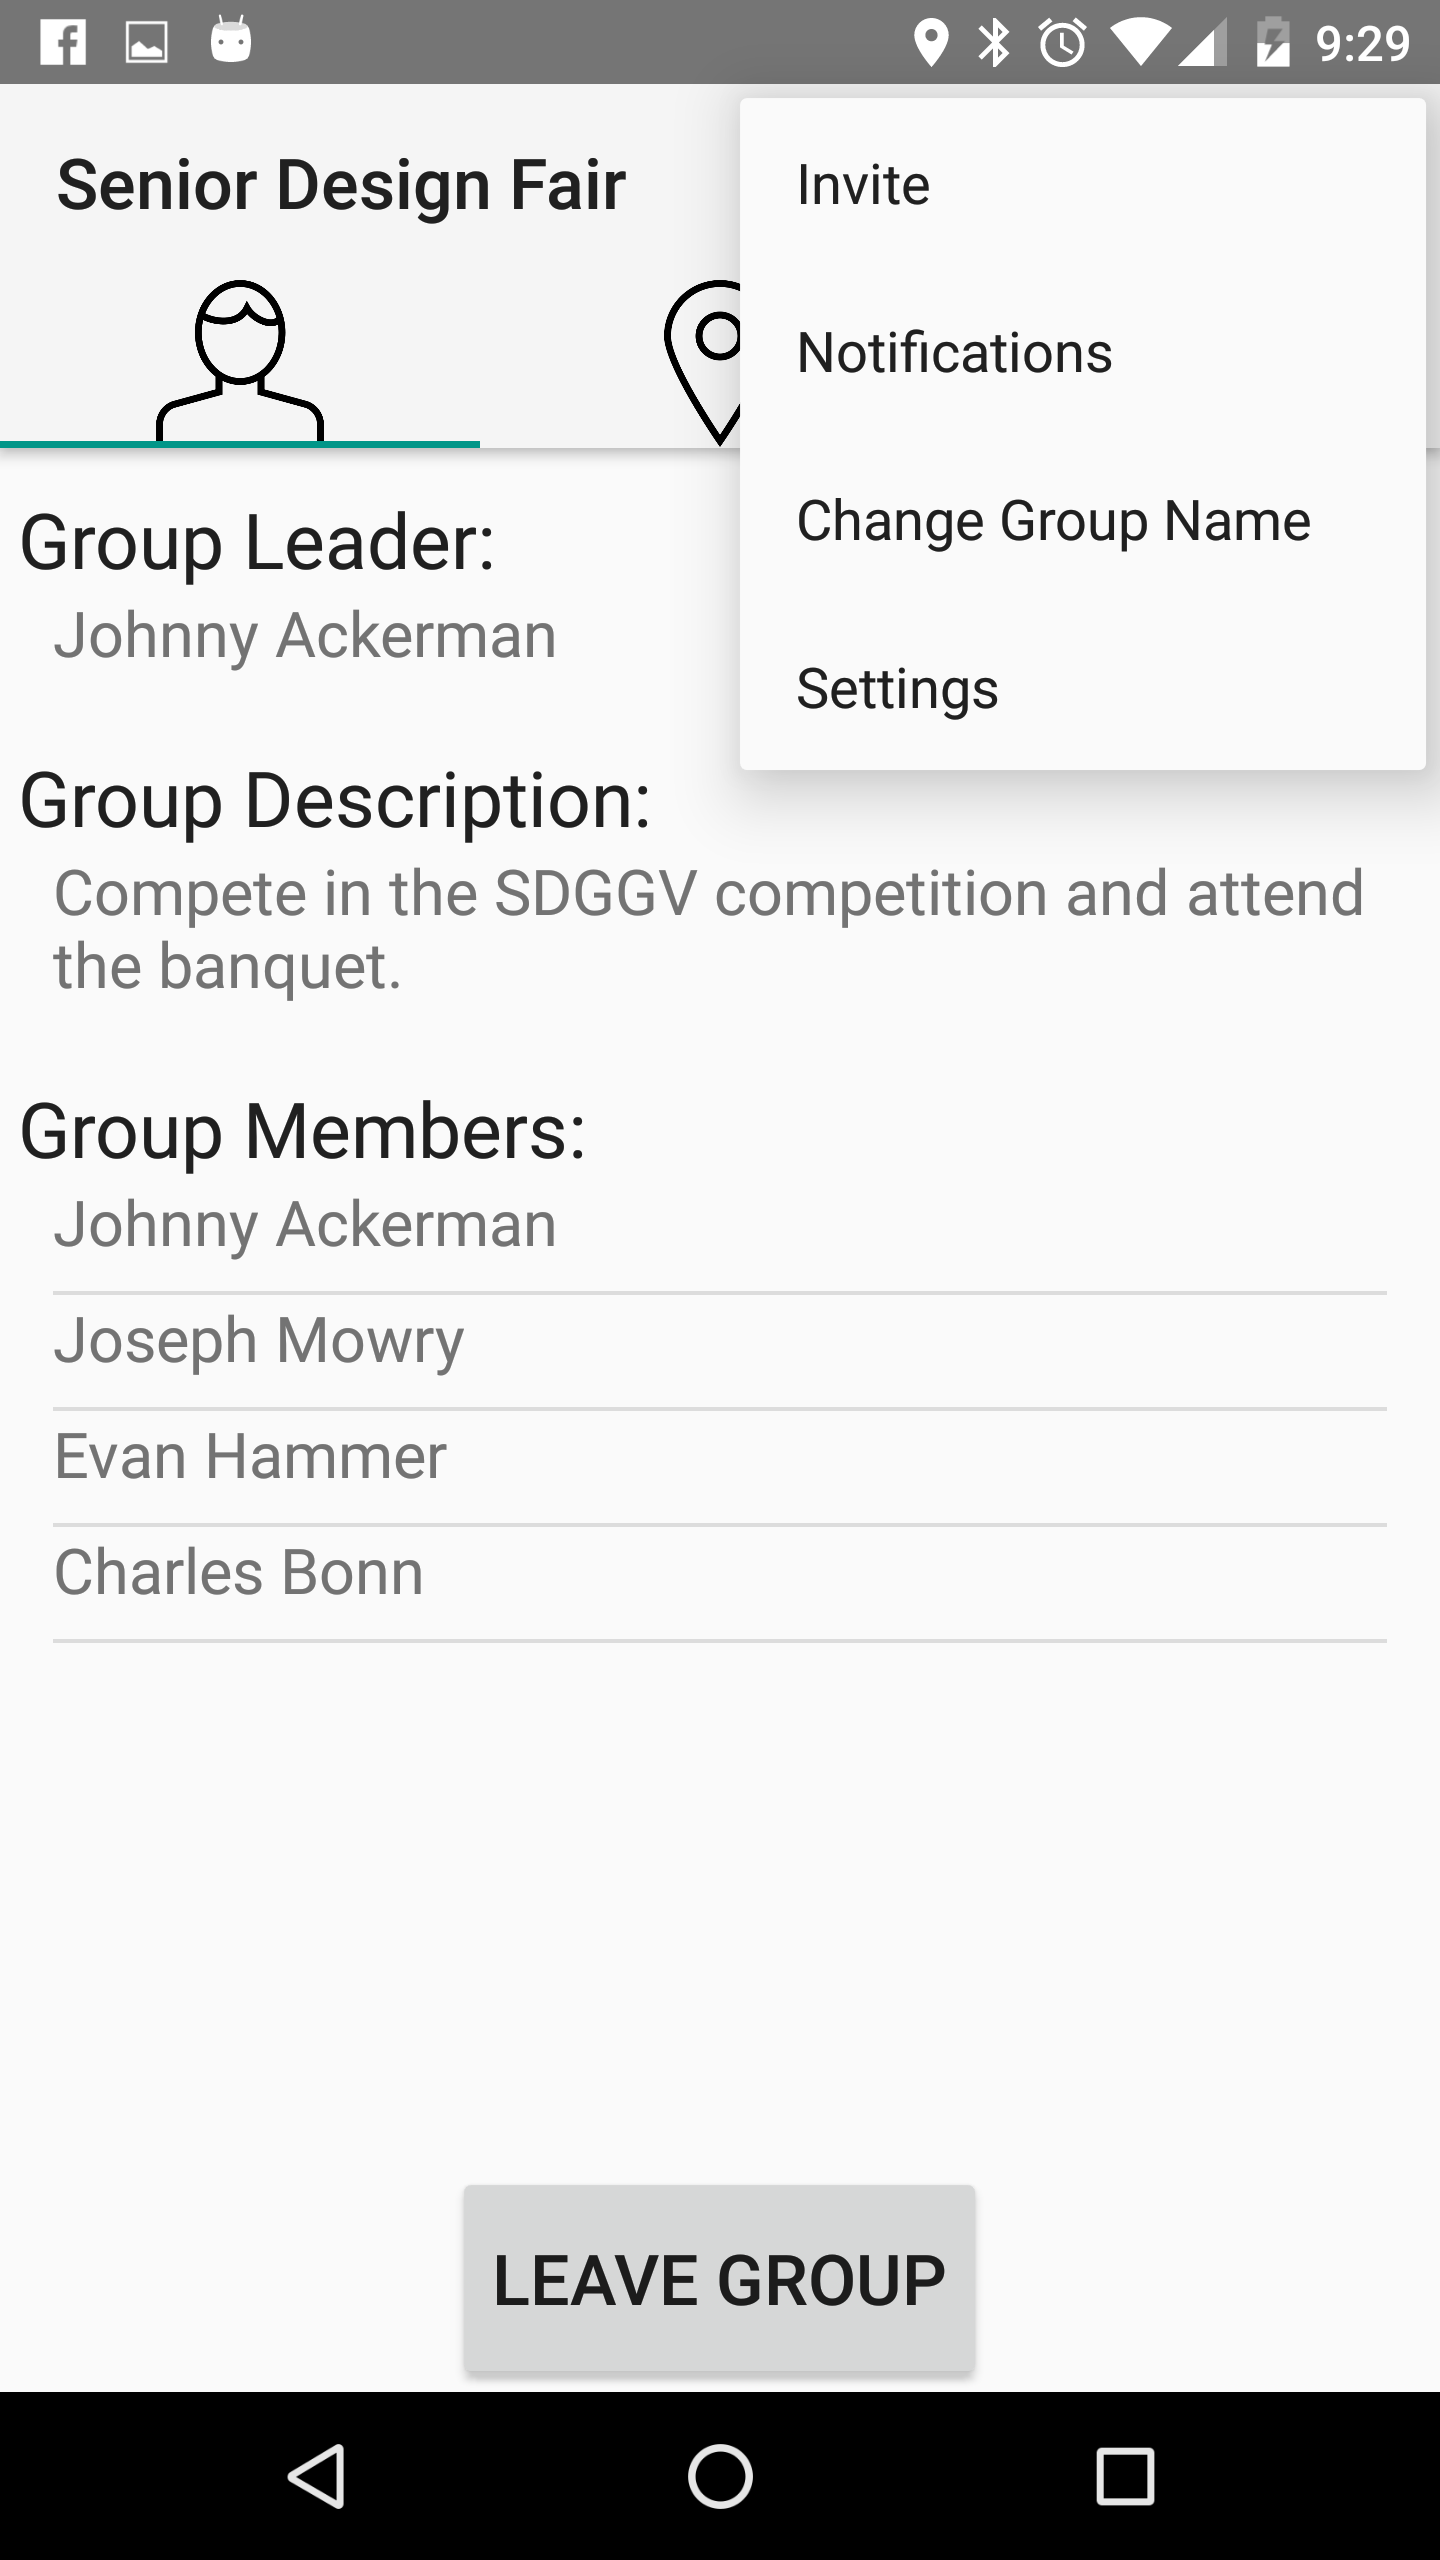
\includegraphics[scale=.1]{Additional/Prototypes/Sprint6/menu.PNG}}
	\fbox{\includegraphics[scale=.1]{Additional/Prototypes/Sprint6/messaging.PNG}}
	\fbox{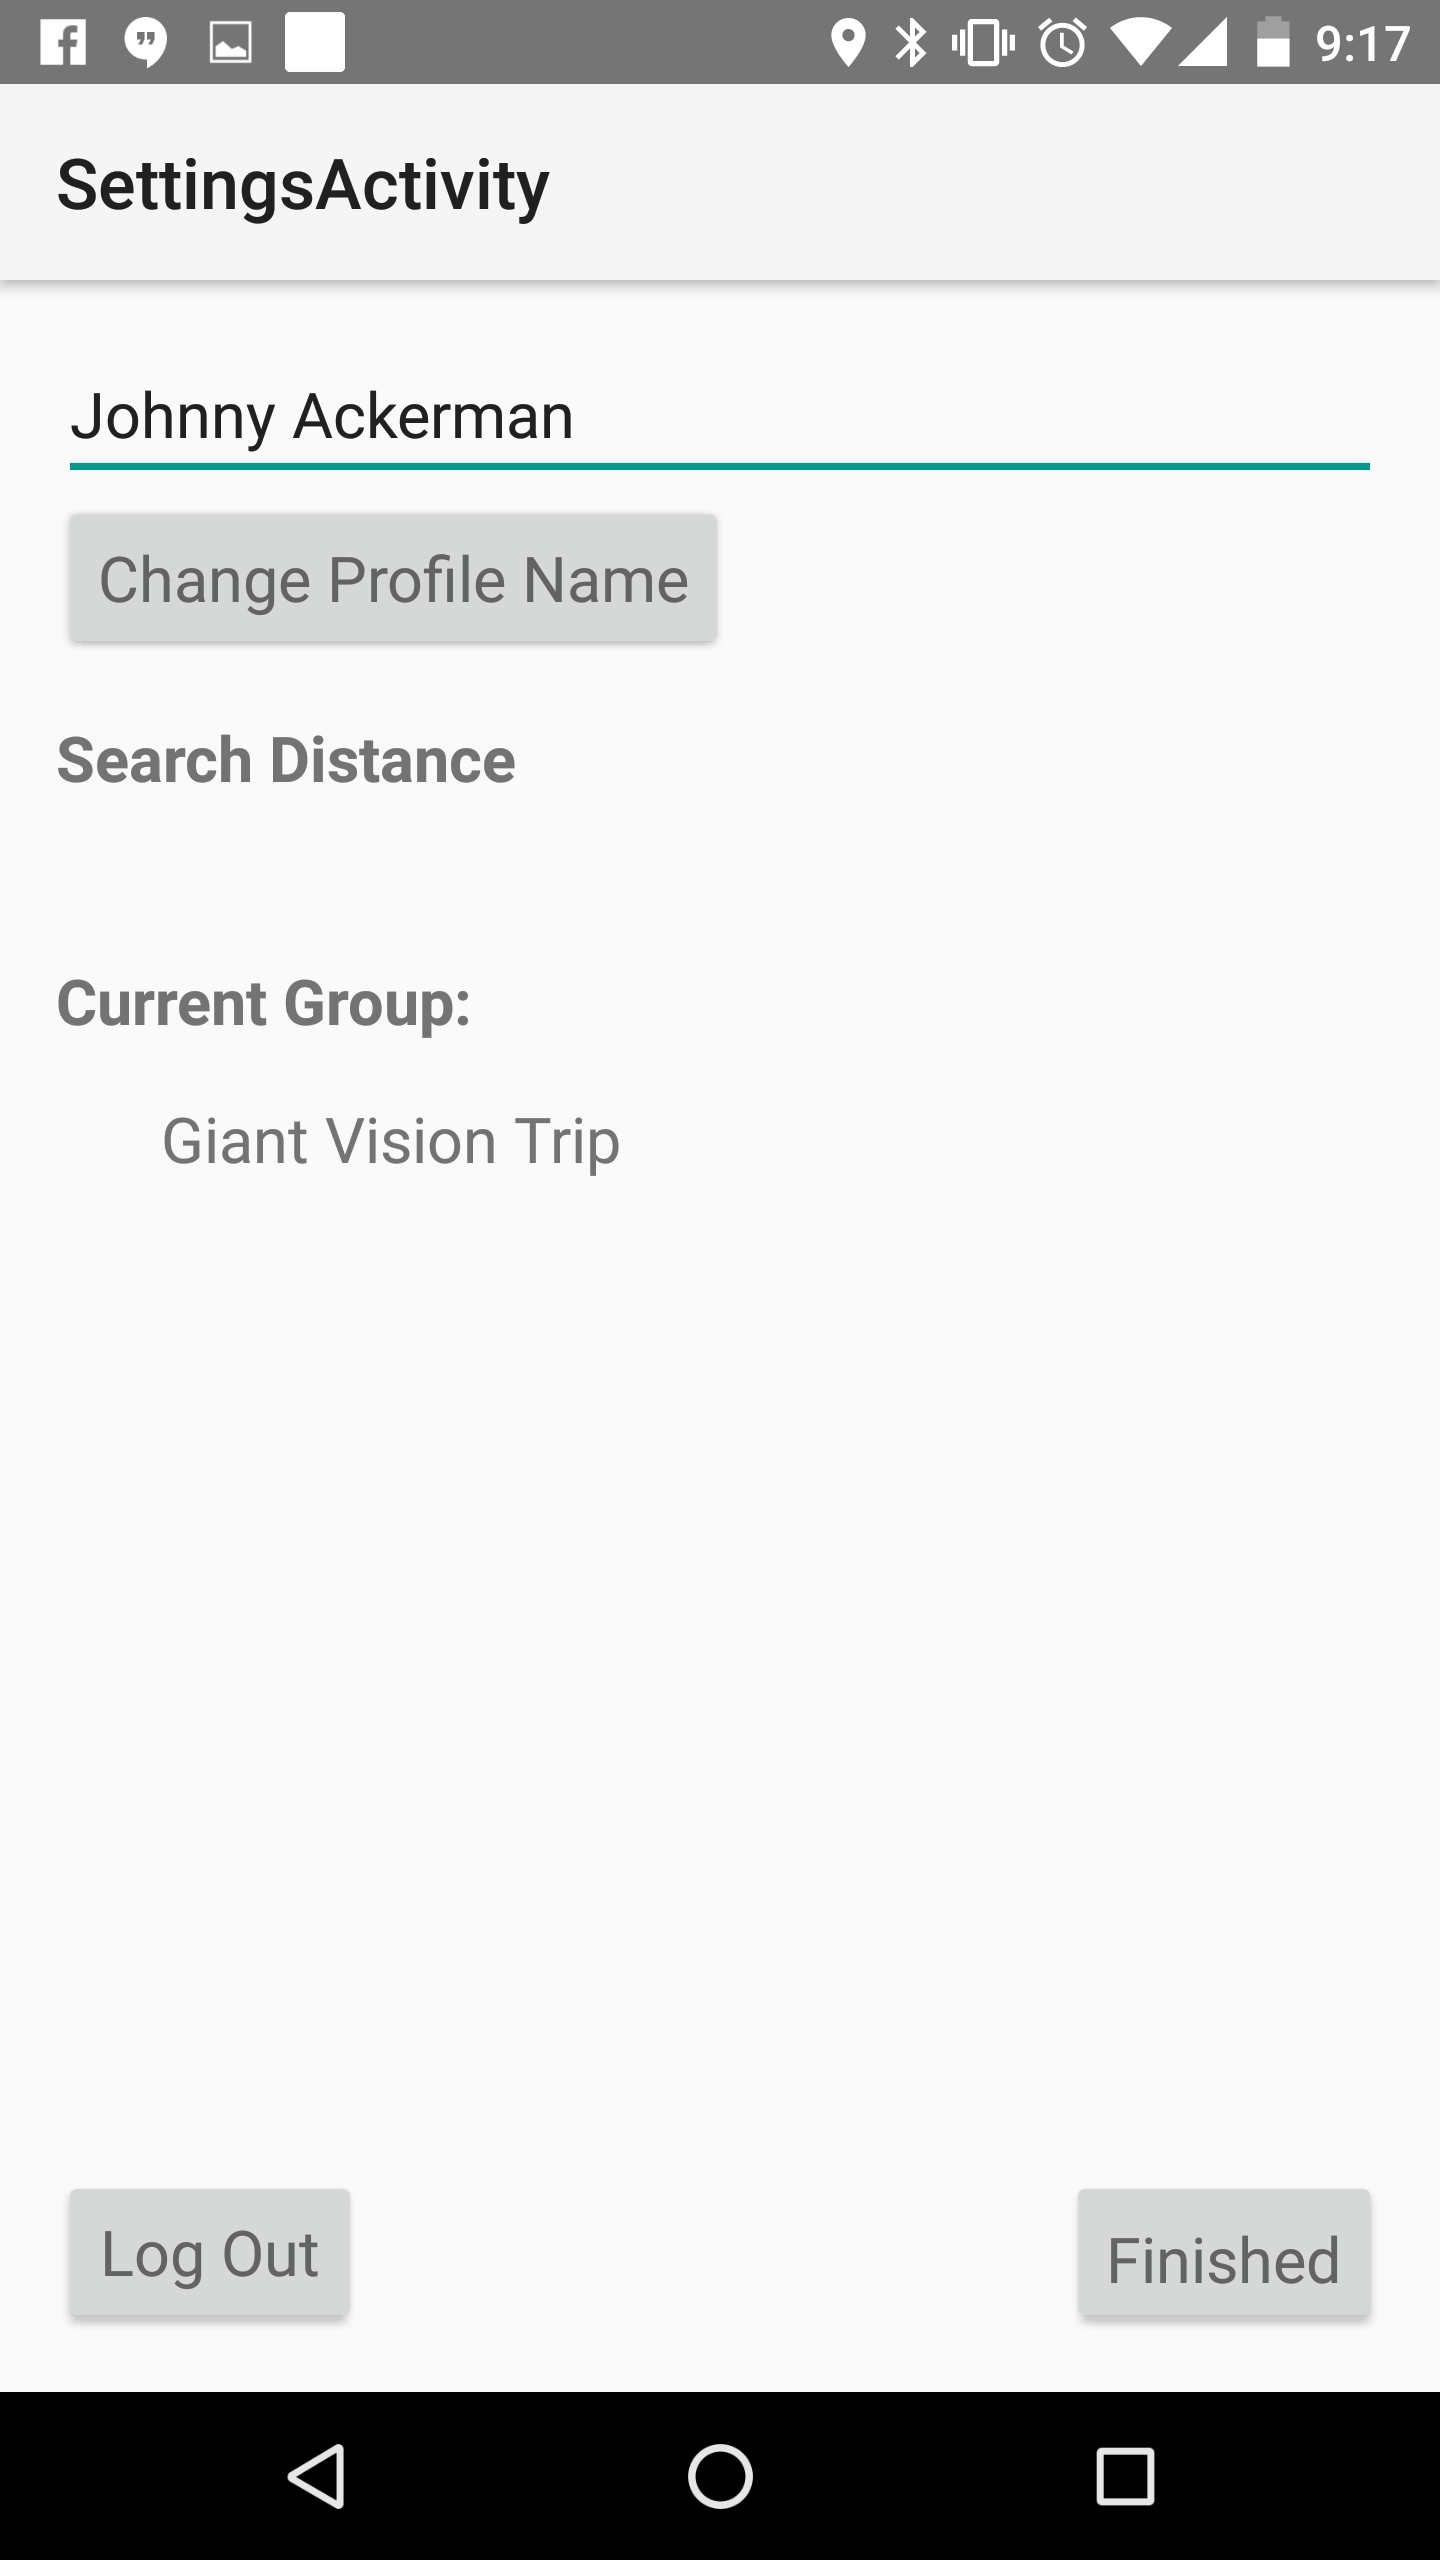
\includegraphics[scale=.1]{Additional/Prototypes/Sprint6/settings.PNG}}
	\end{center}
	\caption{Sprint 6 Prototypes. \label{CommFlow}}
	\end{figure}

\subsection{Deliverable}
\begin{itemize}
	\item Android
	\begin{itemize}
		\item Group Messaging
		\begin{itemize}
			\item Messages now include the names of the sender
			\item Leader can now kick or promote members
			\item Messages now load per group from parse
		\end{itemize}
		\item Broke ground for notification system
		\begin{itemize}
			\item created tab system for invites and accepts
			\item created fragments for invite and confirm
			\item created model for notification system
			\item items can be transferred from the invite fragment to the confirm fragment
		\end{itemize}
		\item Group Management Tools
		\begin{itemize}
			\item Leader can now kick a member
			\item Leader can now promote a member
			\item fixed leader bug, now leader loads properly
		\end{itemize}
		\item Giant Vision
		\begin{itemize}
			\item Pitch complete
			\item Logo finalized and printed
			\item Video backup created
		\end{itemize}
	\end{itemize}
\end{itemize}
\subsection{Backlog}
\begin{description}
	\item[Week 1] \hfill
	\begin{itemize}
		\item Android
		\begin{itemize}
			\item Messaging
			\begin{itemize}
				\item Messages now include the names of the sender
				\item Leader can now kick or promote members
				\item Messages now load per group from parse
			\end{itemize}
			\item Group Management Tools
			\begin{itemize}
				\item Leader can now kick a member
				\item Leader can now promote a member
			\end{itemize}
			\item Facebook and Twitter log-in
			\item Location
			\begin{itemize}
				\item Update location automatically using service
				\item Set Group Location
			\end{itemize}
		\end{itemize}
	\end{itemize}
	
  \item[Week 2] \hfill
		\begin{itemize}
		\item Android
		\begin{itemize}
			\item fixed leader bug, now leader loads properly
			\item broke ground for notification system
			\begin{itemize}
				\item created tab system for invites and accepts
				\item created fragments for invite and confirm
				\item created model for notification system
				\item items can be transferred from the invite fragment to the confirm fragment
			\end{itemize}
			\item Option Menu's added 
			\begin{itemize}
				\item group join now has an option menu
				\item settings activity moved to option menu
				\item Group name can be changed in option menu
				\item option menu is different if you are a group leader
				\item option menu leads to invite system
				\item option menu leads to blank notification page
			\end{itemize}
			\item Reformatted settings activity
			\begin{itemize}
				\item now displays and can change display name
				\item displays a current group if in one
				\item added a finish button for clarity
			\end{itemize}
		\end{itemize}
		\item Cloud code
		\begin{itemize}
			\item Safe group operations(leaving/joining group)
		\end{itemize}
	\end{itemize}
  
  \item[Week 3] \hfill
		\begin{itemize}
		\item Giant Vision Competition
		\begin{itemize}
			\item Create the pitch
			\item Create expo supporting materials
		\end{itemize}
		\item Android
		\begin{itemize}
			\item Notification and invite system incomplete
		\end{itemize}
	\end{itemize}
\end{description}

\subsection{Success/Fail}
\begin{itemize}
	\item Android
	\begin{itemize}
		\item Facebook and Twitter log-in incomplete
		\item Notification and invite system incomplete
	\end{itemize}
	\item Misc
	\begin{itemize}
		\item Did not place at the Giant Vision Competition
	\end{itemize}
\end{itemize}

  %% All tracks
% !TEX encoding = UTF-8 Unicode
% !TEX root = DesignDocument.tex

\chapter{Release -- Setup -- Deployment}
After the proper licenses are attained. The both Android and iOS will be prepared for release in their respective app stores. This is much more difficult to do for the Apple Play Store due to stricter requirements on app quality. Once the apps are release, updates will also be available to download though each respective store.


\section{Deployment Information and Dependencies}
There are no dependencies that need to be installed after app installation. The app will available in the app store for download.



\section{Setup Information}
The app will be down loadable from Google Play Store, or from the Apple Play Store, as a ready to run package.

For testing, a device may be connected to a computer running Android studio or xCode, depending on an Android or Apple device respectively. After the device is connected and the proper drivers are installed (if applicable) the app may be installed using the IDE to the device for whichever version the IDE was currently running.



\section{System  Versioning Information}
The Following is our versioning for our app during development. Due to being before release, the both iOS and Android are still in their 0 build. Each sprint during the 0 build is denoted by the second number. If there were any substantial changes that required an additional note, it would be denoted by the third number. Thus making our versions look like pre-release(0).sprint(x).substantial change(0), as an example.\\



Current Version [0.3.0]
\vspace*{5mm}

{\color{SDColor5}
\noindent
\textit{Prepared By:}\\
\textit{Daniel Andrus}\\
\textit{Evan Hammer}
}
\vfill
\noindent
{\color{SDColor3} \textit{\textbf{iOS App Version History}}}\\
\begin{tabular}{|>{\raggedright}p{1.5cm}|>{\raggedright}p{1.5cm}|>{\raggedright}p{9cm}|}
\hline
\textit{\textbf{Date}} &  \textit{\textbf{Version}} & \textit{\textbf{Comments}}\tabularnewline
\hline
 \textit{\textbf{10/1/15}} & \textit{0.0.0} & \textit{Napkin Designs and Ideas}\tabularnewline
 \hline
  \textit{\textbf{11/3/15}} & \textit{0.1.0} & \textit{App Initialization, basic framework}\tabularnewline
 \hline
 \textit{\textbf{12/11/15}} & \textit{0.2.0} & \textit{mapping and group functionality}\tabularnewline
\hline
 \textit{\textbf{1/18/16}} & \textit{0.3.0} & \textit{Model Restructure}\tabularnewline
 &  & \tabularnewline
\hline
\end{tabular}
\vfill

\break


Current Version [0.6.0]
\vspace*{5mm}

{\color{SDColor5}
\noindent
\textit{Prepared By:}\\
\textit{Johnathan Ackerman}\\
\textit{Daniel Andrus}\\
\textit{Charles Bonn}\\
\textit{Evan Hammer}\\
\textit{Joseph Mowry}
}
\vfill
\noindent
{\color{SDColor3} \textit{\textbf{Android App Version History}}}\\
\begin{tabular}{|>{\raggedright}p{1.5cm}|>{\raggedright}p{1.5cm}|>{\raggedright}p{9cm}|}
\hline
\textit{\textbf{Date}} &  \textit{\textbf{Version}} & \textit{\textbf{Comments}}\tabularnewline
\hline
 \textit{\textbf{10/1/15}} & \textit{0.0.0} & \textit{Napkin Designs and Ideas}\tabularnewline
 \hline
  \textit{\textbf{11/3/15}} & \textit{0.1.0} & \textit{App Initialization and Basic Framework}\tabularnewline
 \hline
 \textit{\textbf{12/11/15}} & \textit{0.2.0} & \textit{Group Functionality}\tabularnewline
\hline
 \textit{\textbf{1/18/16}} & \textit{0.3.0} & \textit{Bug Fixes and Model Reorganization}\tabularnewline
\hline
 \textit{\textbf{2/12/16}} & \textit{0.4.0} & \textit{Group Messaging and Mapping}\tabularnewline
\hline
 \textit{\textbf{2/18/16}} & \textit{0.5.0} & \textit{Theme Overall and Bug Fixes}\tabularnewline
\hline
\textit{\textbf{5/1/16}} & \textit{0.6.0} & \textit{Leader Controls}\tabularnewline
 &  & \tabularnewline
\hline
\end{tabular}
\vfill

After release, our application will finally hit build 1. From this stage, any further sprints will of course increment the version, and if any bug fixes are required to be public during a sprint, we will increment the last number previously reserved for substantial changes in a sprint.  %% Normally not research track
% !TEX root = SystemTemplate.tex

\chapter{User Documentation}

This section should contain the basis for any end user documentation for the system. 
 End user documentation would cover the basic steps for setup and use of the system. 
 It is likely that the majority of this section would be present in its own document 
to be delivered to the end user.  However, it is recommended the original is contained 
and maintained in this document. 

%\newpage   %% 
%%  The user guide can be an external document which is included here if necessary ...
%%  a single source is the way to go.

\section{User Guide}

The source for the user guide can go here.    You have some options for how to handle the user docs.  If you have some {\tt newpage} commands around the guide then you can just print out those pages.   If a different formatting is required, then have the source in a separate file {\tt userguide.tex} and include that file here.  That file can also be included into a driver (like the senior design template) which has the client specified formatting.  Again, this is a single source approach.   


%% \newpage  %%  if needed ...
\section{Installation Guide}


%% \newpage  %%  if needed ...
\section{Programmer Manual}

 %% All tracks
% !TEX root = DesignDocument.tex


\chapter{Class Index}
% !TEX encoding = UTF-8 Unicode
% !TEX root = DesignDocument.tex


\section{Class List}
Here are the classes, structs, unions and interfaces with brief descriptions\-:\begin{DoxyCompactList}
\item\contentsline{section}{\hyperlink{class_poly}{Poly} }{\pageref{class_poly}}{}
\end{DoxyCompactList}

\chapter{Class Documentation}
\hypertarget{class_poly}{\section{Poly Class Reference}
\label{class_poly}\index{Poly@{Poly}}
}
\subsection*{Public Member Functions}
\begin{DoxyCompactItemize}
\item 
\hyperlink{class_poly_aa3def076b74bed67904976ad4f9fe9b1}{Poly} ()
\item 
\hyperlink{class_poly_a2f8530284140c31c0aa391dd4d0b61be}{$\sim$\-Poly} ()
\item 
int \hyperlink{class_poly_a14a7ad77ce612b0c54f531d307ee4b39}{myfunction} (int)
\end{DoxyCompactItemize}


\subsection{Constructor \& Destructor Documentation}
\hypertarget{class_poly_aa3def076b74bed67904976ad4f9fe9b1}{\index{Poly@{Poly}!Poly@{Poly}}
\index{Poly@{Poly}!Poly@{Poly}}
\subsubsection[{Poly}]{\setlength{\rightskip}{0pt plus 5cm}Poly\-::\-Poly (
\begin{DoxyParamCaption}
{}
\end{DoxyParamCaption}
)}}\label{class_poly_aa3def076b74bed67904976ad4f9fe9b1}
My constructor \hypertarget{class_poly_a2f8530284140c31c0aa391dd4d0b61be}{\index{Poly@{Poly}!$\sim$\-Poly@{$\sim$\-Poly}}
\index{$\sim$\-Poly@{$\sim$\-Poly}!Poly@{Poly}}
\subsubsection[{$\sim$\-Poly}]{\setlength{\rightskip}{0pt plus 5cm}Poly\-::$\sim$\-Poly (
\begin{DoxyParamCaption}
{}
\end{DoxyParamCaption}
)}}\label{class_poly_a2f8530284140c31c0aa391dd4d0b61be}
My destructor 

\subsection{Member Function Documentation}
\hypertarget{class_poly_a14a7ad77ce612b0c54f531d307ee4b39}{\index{Poly@{Poly}!myfunction@{myfunction}}
\index{myfunction@{myfunction}!Poly@{Poly}}
\subsubsection[{myfunction}]{\setlength{\rightskip}{0pt plus 5cm}int Poly\-::myfunction (
\begin{DoxyParamCaption}
\item[{int}]{a}
\end{DoxyParamCaption}
)}}\label{class_poly_a14a7ad77ce612b0c54f531d307ee4b39}
my own example function fancy new function

new variable 

The documentation for this class was generated from the following file\-:\begin{DoxyCompactItemize}
\item 
hello.\-cpp\end{DoxyCompactItemize} 








%\hypertarget{class_BaseModel.Android}
%\hypertarget{class_BaseModel.LoadCallback.Android}
%\hypertarget{class_BaseModel.SaveCallback.Android}
%\hypertarget{class_BuildConfig.Android}
%\hypertarget{class_CreateAccountActivity.Android}
%\hypertarget{class_CrowdControlApplication.Android}
%\hypertarget{class_EventFragment.Android}
%\hypertarget{class_GroupCreateActivity.Android}
%\hypertarget{class_GroupInfoFragment.Android}
%\hypertarget{class_GroupJoinActivity.Android}
%\hypertarget{class_GroupModel.Android}
%\hypertarget{class_GroupNavigationActivity.Android}}
%\hypertarget{class_LoginActivity.Android}
%\hypertarget{class_LoginController.Android}
%\hypertarget{class_MapFragment.Android}
%\hypertarget{class_MessagingFragment.Android}
%\hypertarget{class_ParseBaseModel.Android}
%\hypertarget{class_ParseGroupModel.Android}
%\hypertarget{class_ParseUserModel.Android}
%\hypertarget{class_ParseUserProfileModel.Android}
%\hypertarget{class_R.Android}
%\hypertarget{class_R.anim.Android}
%\hypertarget{class_R.attr.Android}
%\hypertarget{class_R.boo.Android}
%\hypertarget{class_R.color.Android}
%\hypertarget{class_R.dimen.Android}
%\hypertarget{class_R.drawable.Android}
%\hypertarget{class_R.id.Android}
%\hypertarget{class_R.integer.Android}
%\hypertarget{class_R.layout.Android}
%\hypertarget{class_R.menu.Android}
%\hypertarget{class_R.minimap.Android}
%\hypertarget{class_R.plurals.Android}
%\hypertarget{class_R.raw.Android}
%\hypertarget{class_R.string.Android}
%\hypertarget{class_R.style.Android}
%\hypertarget{class_R.styleable.Android}
%\hypertarget{class_SignupActivity.Android}
%\hypertarget{class_UserModel.Android}
%\hypertarget{class_UserProfileModel.Android}
%\hypertarget{class_WelcomeAcitivity.Android}


  %% All tracks
% !TEX encoding = UTF-8 Unicode
% !TEX root = DesignDocument.tex

\chapter{Business Plan}


\includepdf{Additional/BusinessPlan/bowTapsCrowdControlBusinessPlan.pdf}

%\section{Business Model}

%\section{Market and Competition}

%\section{Regulatory environment}

%\section{Intellectual Property and Freedom to Operate}

%\section{Management Team and Advisors}

%\section{Sources and Uses of Capital}

%\section{Financial Statements}

\%section{Metrics and Milestones}

%\section{Exit Plan}

   %% Entrepreneur track only 
%% !TEX root = SystemTemplate.tex

\chapter{Experimental Log}

For research projects one needs to keep a log of all research/lab activities.   

%% If you have multiple labs, you may want to break the labs into sections, check 
%% with the profession on format.
%% \section{Lab 1}

\begin{description}
\item [10/15/15]  Ran modified filter on data sets 1 - 6.  Results were ...
\item [10/17/15]  Changed tolerance on sensor and collected data.  These ...
\end{description}   %% Research track  only
%% !TEX root = SystemTemplate.tex

\chapter{Research Results}

This chapter describes the results and conclusions of your research.   This would be the final report for a research project.  

\section{Result 1}

\section{Result 2}

\section{Conclusions}

\section{Further work}    %% Research track  only

\bibliographystyle{plain}
\bibliography{designrefs.bib}
\addcontentsline{toc}{chapter}{Bibliography}


% We want to add the Software agreement to the end and number the
% pages separately from the document.  We don't want to do a standard
% chapter heading, but we do want it to appear in the table of contents
% and in the index used for on-line viewing.  We defined the \agreement
% macro to set things up for us.
\agreement

\chapter{Software Agreement}
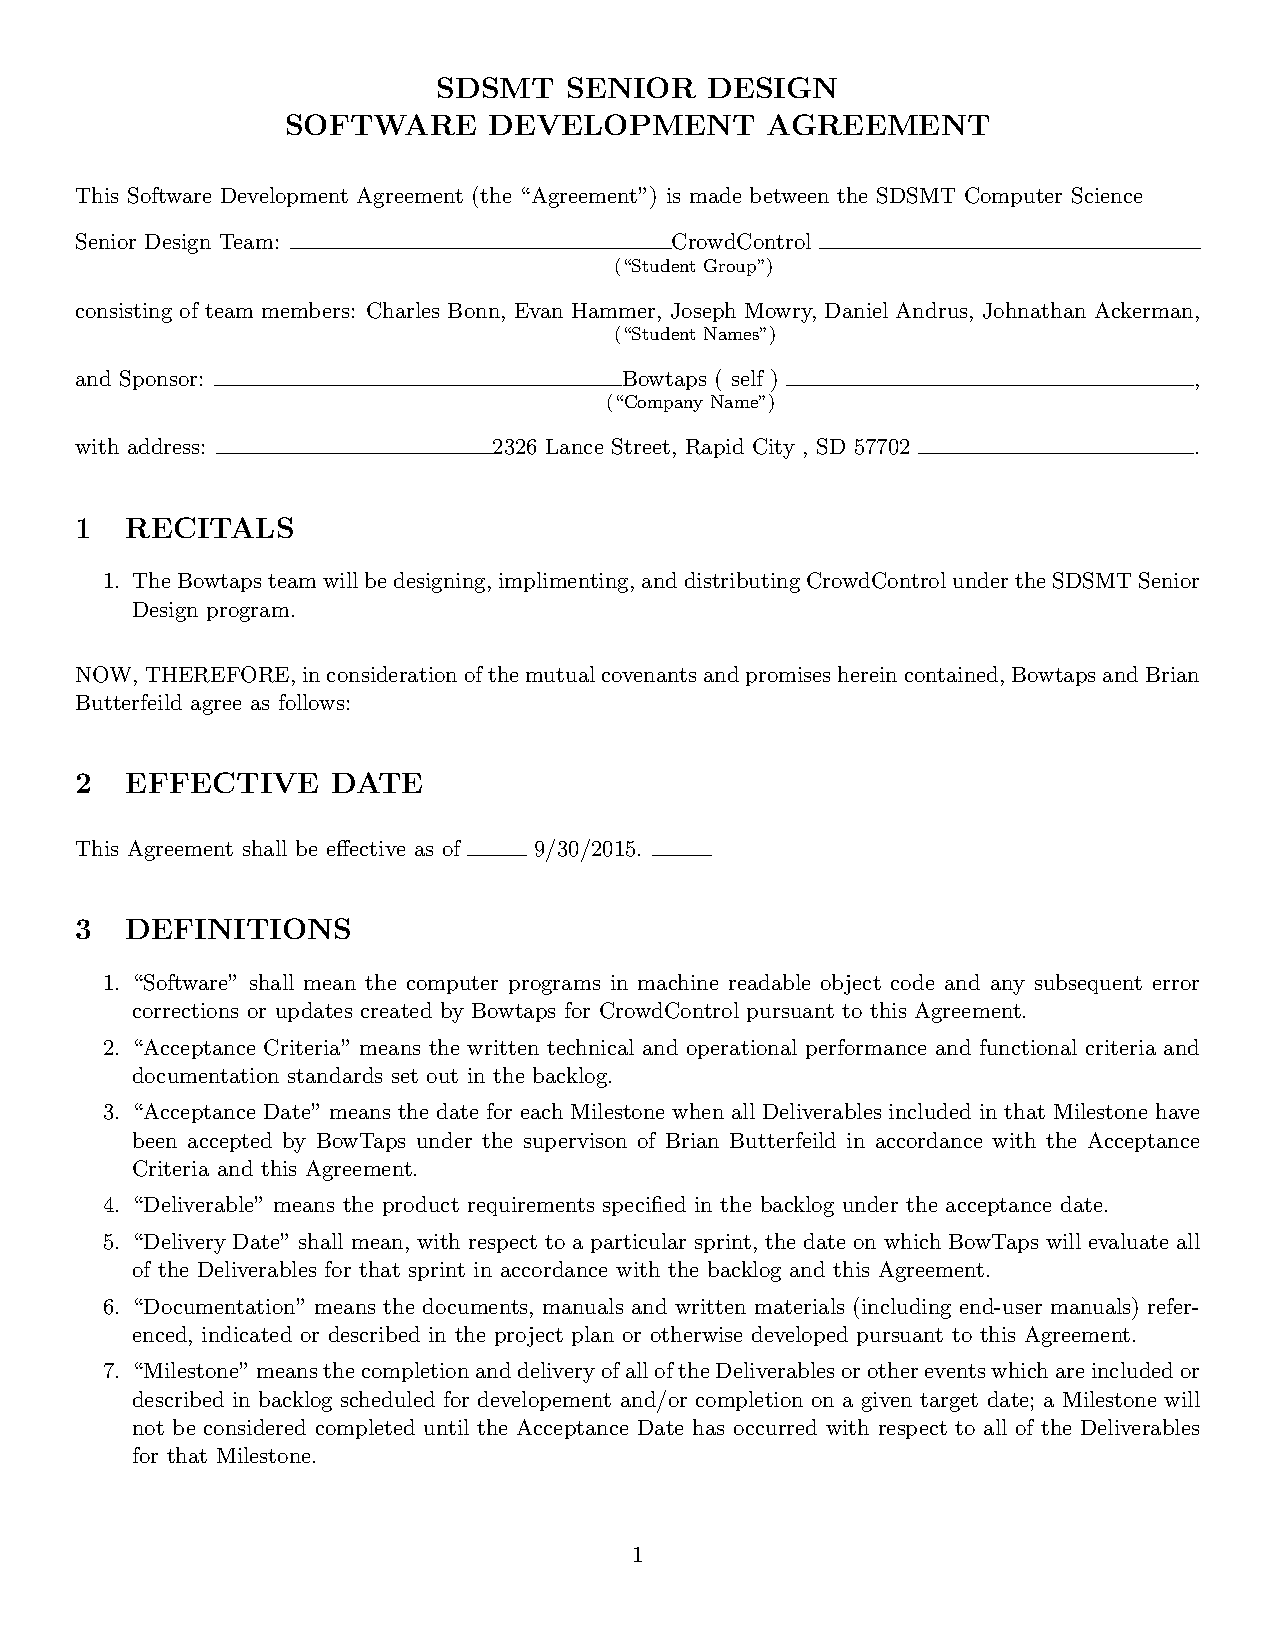
\includepdf[pages={1-5}]{Additional/SoftwareContract/SoftwareContract-signed.pdf}

% In our style file, appendices are numbered with capital letters
\appendix

\chapter{Product Description}
% !TEX root = DesignDocument.tex


%Write a description of the product to be developed.
%Use sectioning commands as neccessary.
%\vspace{2\baselineskip}

%\centerline{\Large {\bf NOTE:} {\em This is part of the contract.}}

CrowdControl is a group management application that will be an application that has gps features, group messaging, group management features.

\section{GPS Features}

\subsection{Group Members}

The Group member gps features will allow for users to track other users in the same group as they are. This will be under user permission to allow other user to see there location.

\subsection{Suggestions}

The suggestion side of the GPS will take a user or group location and give even suggestions of places to go or things to do in the area of the group.

\section{Group Messaging}

Integrated group messaging on a single platform uniform to iOS and android. 

\section{Group Manangement Features}

This will allow for members to join a group, add a member to a group, and leave a group.

\section{Parse Features}

Parse will be used to store user data and group data.


%\chapter{Publications}   %% Research track 
%% !TEX root = SystemTemplate.tex


Research Track:  
This chapter will include any publications generated from the research.  Most likely these will be preprints and one will just include the pdf.

%\includepdf[pages={1-5}]{Pub1.pdf}



\chapter{Sprint Reports}
% !TEX root = DesignDocument.tex


%\section{Sprint Report \#1}

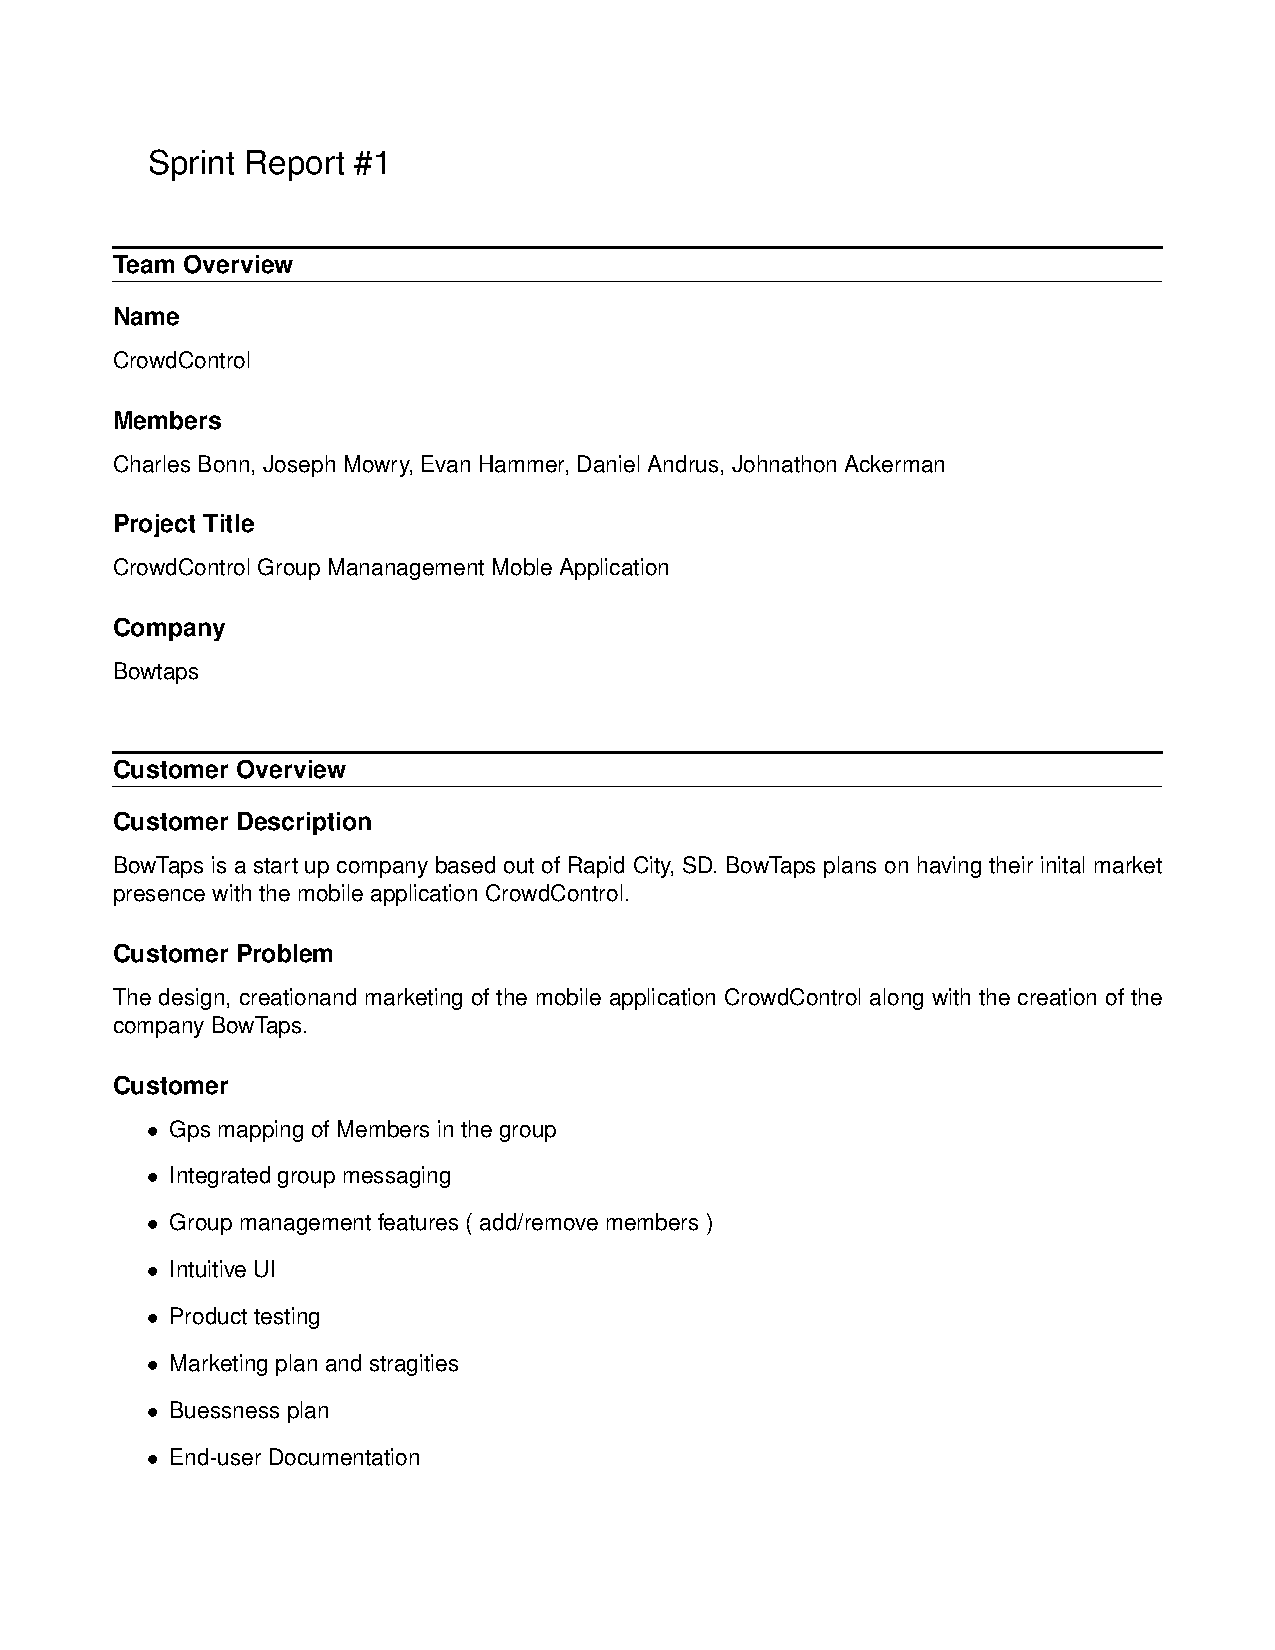
\includepdf[pages=-]{Additional/sprints/sprint1_wrapper.pdf}

%\section{Sprint Report \#2}

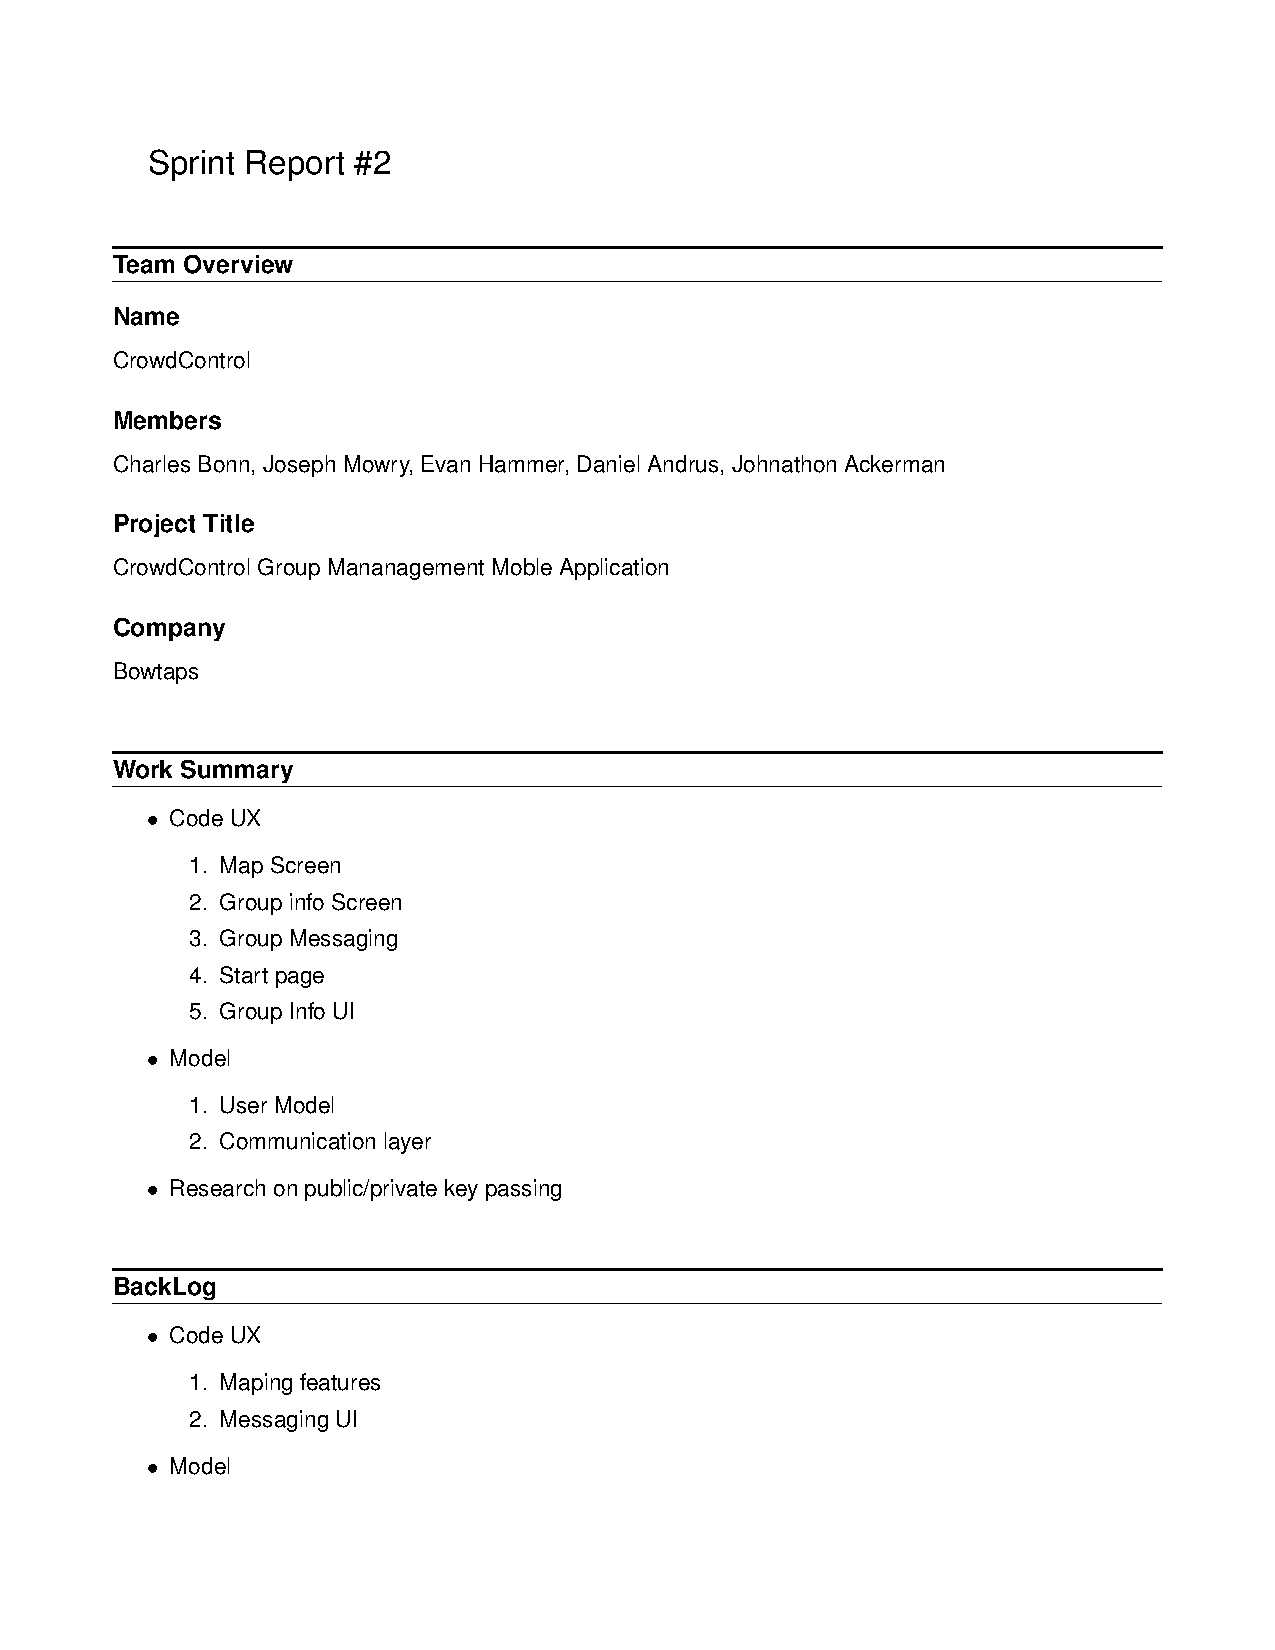
\includepdf[pages=-]{Additional/sprints/sprint2_wrapper.pdf}

%\section{Sprint Report \#3}

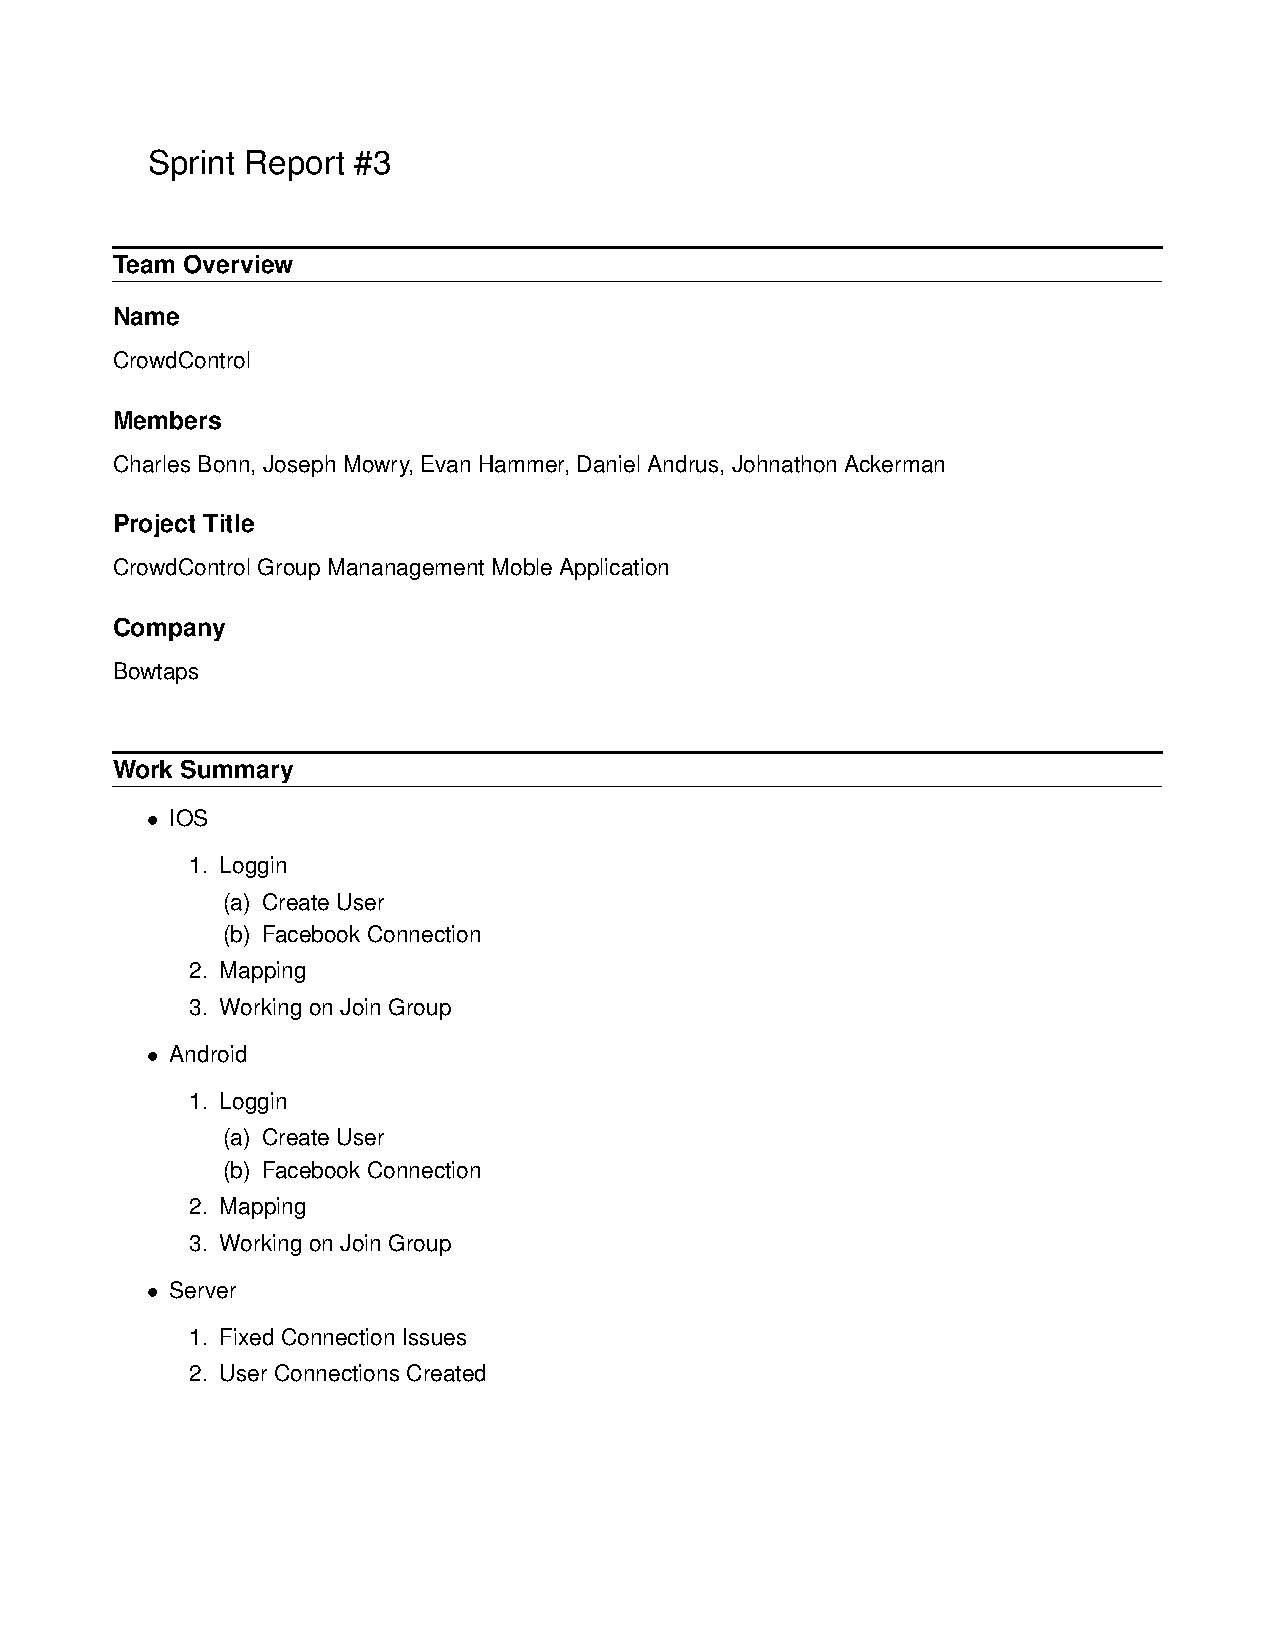
\includepdf[pages=-]{Additional/sprints/sprint3_wrapper.pdf}

%\section{Sprint Report Winter Sprint}

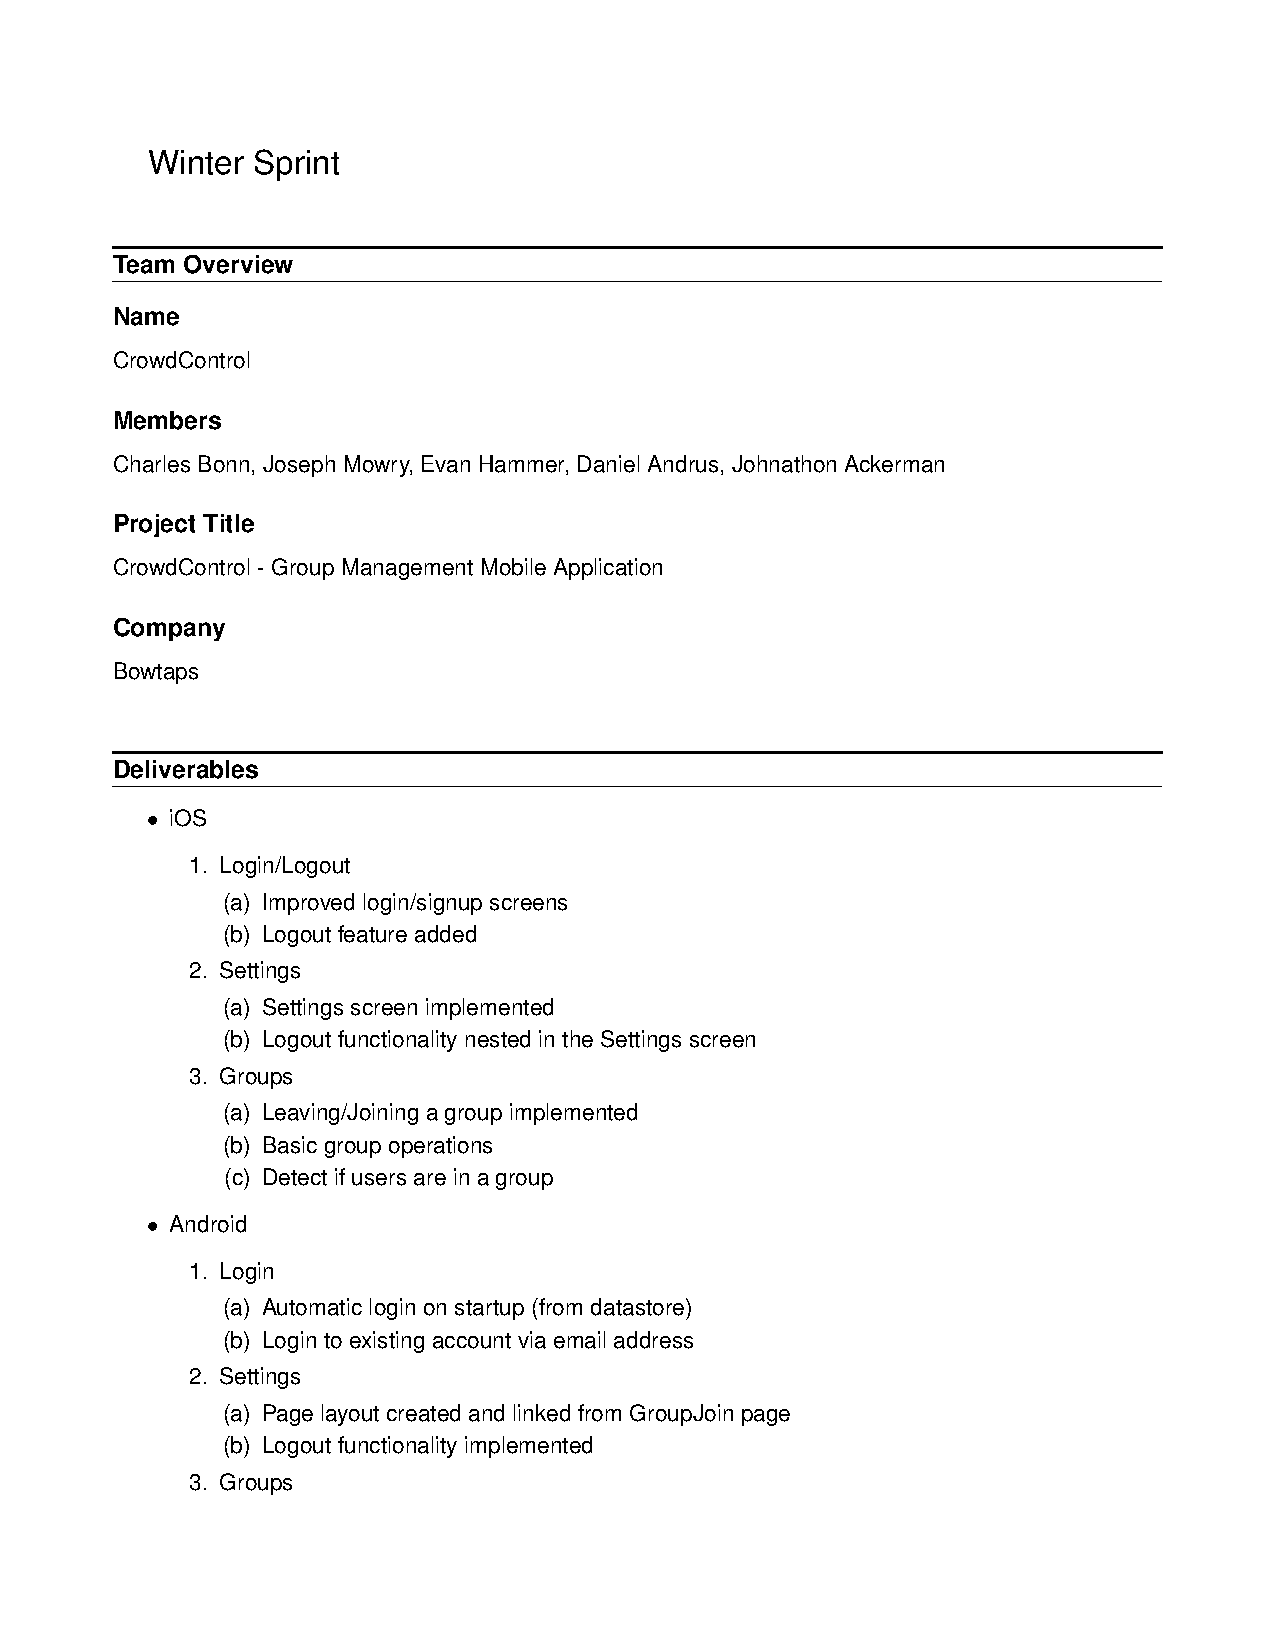
\includepdf[pages=-]{Additional/sprints/wSprintWrapper.pdf}

%\section{Sprint Report Winter Sprint}

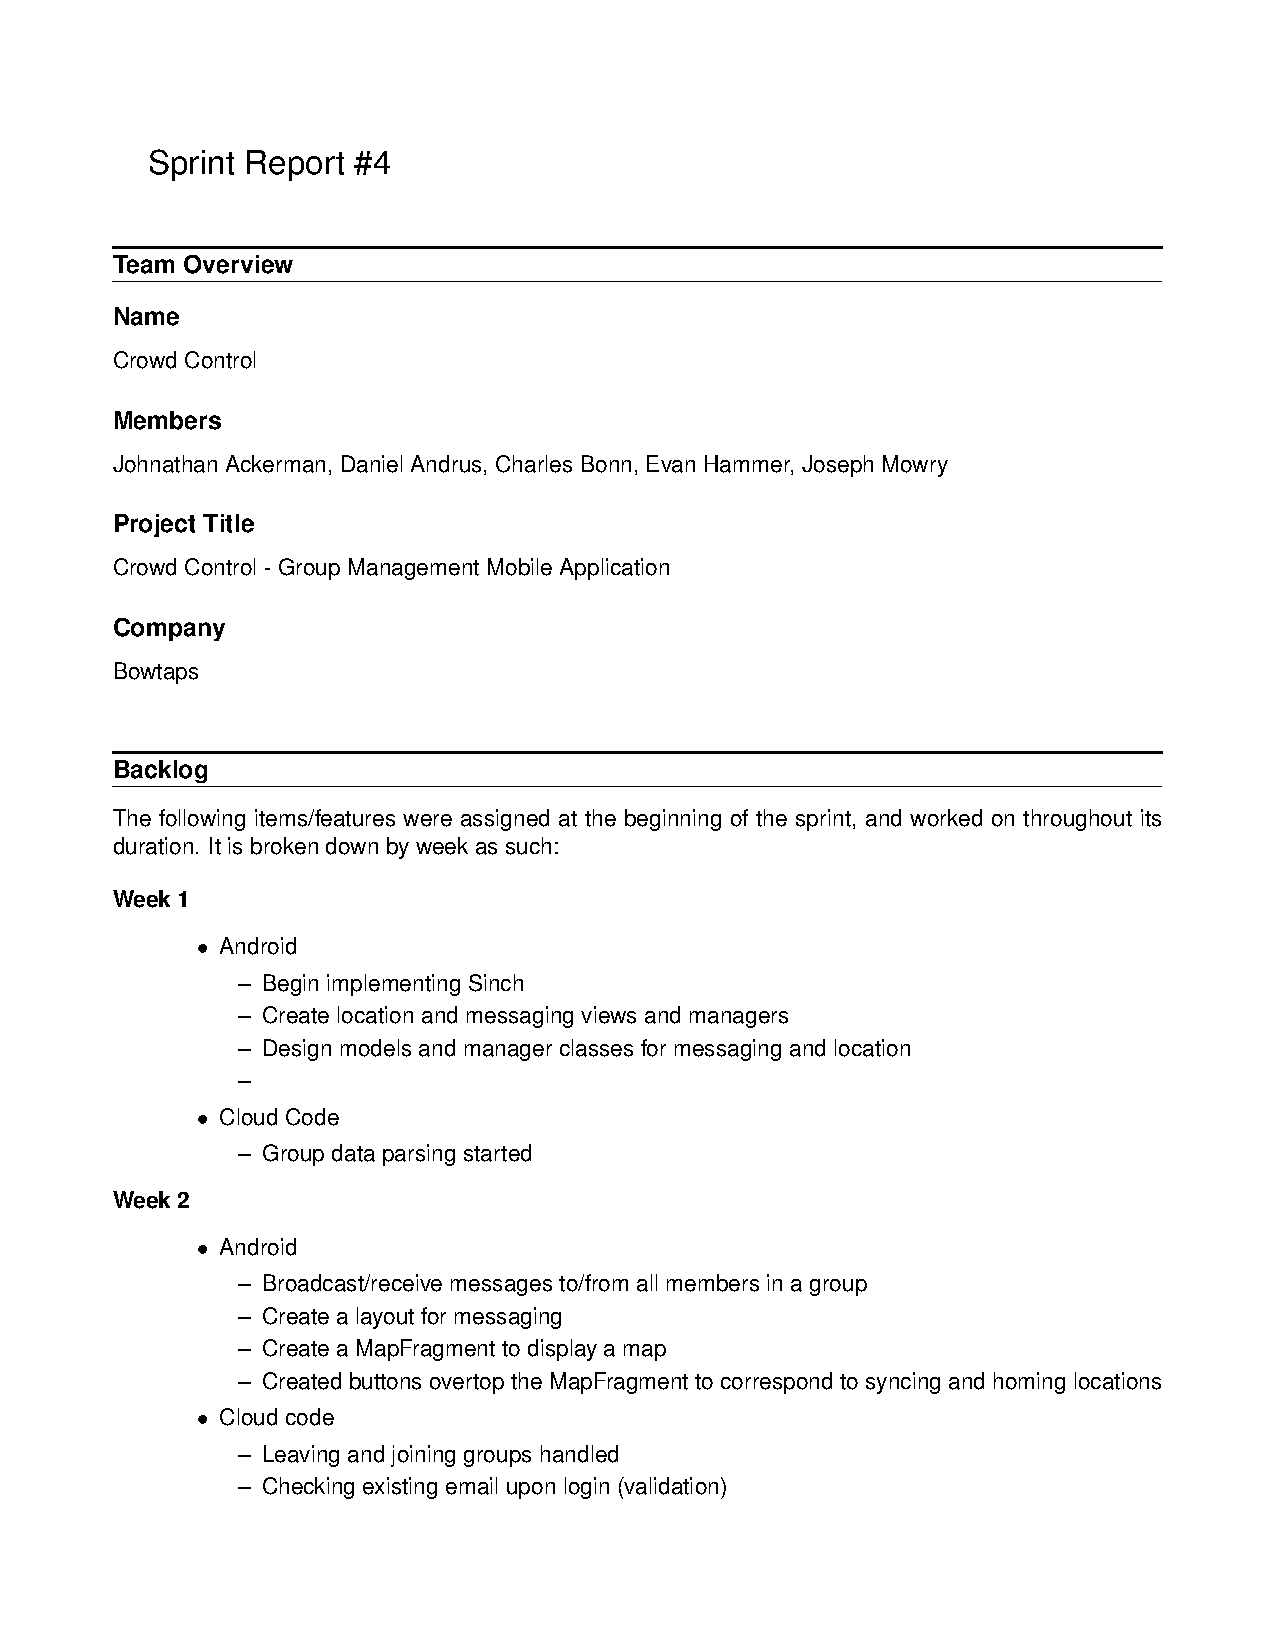
\includepdf[pages=-]{Additional/sprints/Sprint4Wrapper.pdf}



\chapter{Industrial Experience and Resumes}
% !TEX root = SystemTemplate.tex


\section{Resumes}

Below are the resumes for the group members: Johnathon Ackerman, Daniel Andrus, Charles Bonn, Evan Hammer, and Joseph Mowry.

%    \includepdf[pages={1}]{report.pdf}  %% example of limited page include

%     \includepdf{resume1.pdf}
%     \includepdf{resume2.pdf}
%     \includepdf{resume3.pdf}
\includepdf{resumes/JohnathonAckermanResume.pdf}
\includepdf{resumes/DanAndrusResume.pdf}
\includepdf{resumes/NickBonnResume.pdf}
\includepdf{resumes/EvanHammerResume.pdf}
\includepdf{resumes/JosephMowryResume.pdf}

\section{ABET:  Industrial Experience Reports}
As a group we have attended the  SD Engineering Accelerator. We have compeated in multiple business plan competitions including:
	\begin{itemize}
	\item{Butterfield Cup}
	\item{SD Innovation Expo Business Plan Competition}
	\item{2015 SD Mines CEO Student Business Plan Competition}
	\end{itemize}
We also have also have and regular meetings with SDSMT EIR's to help format our buisness plan and Crowd Control.

\subsection{Johnathon Ackerman}

 I have had no Internship experience. However, before the project Crowd Control, I worked with C++, lisp, and python. I have worked with Visual Studios on Windows side, and Vim and G edit in Linux. 

\subsection{Daniel Andrus}

I first learned the basics of web design and development in high school. After my second year of college, I obtained an internship with FTW Interactive (now known as Red Shed Technologies). Later, I hold a position as Web Developer for 2 years before becoming an intern software developer at 7400 Circuits.

My course experience has ranged from data structures, image processing, database design, web development, group projects, computer graphics (including 3D graphics), mobile app development, and even compression.

\subsection{Charles Bonn}

I currently have little internship experence. What industry experence i do have is HTML. In my personal/professional life i help manage a website and a minecraft server. Though this is work i have worked with HTML and C code. I have also worked with game code that is java based.

\subsection{Evan Hammer}

I am working for Golden West Telecommunications(GW), a rural telecommunications provider in the state of South Dakota.  Since May of 2015 I have been a Software Developer for GW working on both mobile and back-end products.  For the mobile side, I have been working with a product called Cordova that is wrapped with another product called Sencha Touch.  Together these two products allow a developer to use JavaScript, HTML, CSS and more to produce a mobile application for Android, iOS and many other mobile platforms.  I have also written the back-end for this app, using Python and a PostgreSQL Database creating a server-side API for the mobile application.  While I am not working on the mobile application I have spent my time working on other in-house products using languages like Python and JavaScript.  These projects have ranged from updating existing code to ground-up projects.  Also as a Software Developer for GW, I have been tasked with creating some proof of concept work.  This work has ranged from testing possible new services as well as testing new platforms for development.  My work continues to grow and change as I continue to work for Golden West Telecommunications.

\subsection{Joseph Mowry}

In his pirior industry experience, Joseph specialized in C\# development and database management. His employers gave him a solid footing in AGILE and Scrum methodologies, as well as general product development. Though his experience lies primarily on the Visual Studio/C\# side of things, there is a large amount of skill overlap in Android Studio and Java that he can bring to the table for this project.




\chapter{Acknowledgment}
\label{SpecialThanks}  
As a special thanks we would like to thank Brian Butterfeild. His mentouring has made this project possable. \newline
Another thanks goes to Dr. Logar, With out your soft engeneering class this would have never been possable.

\chapter{Supporting Materials}

This document will contain several appendices used as a way to separate out major 
component details, logic details, or tables of information.  Use of this structure 
will help keep the document clean, readable, and organized. 



% chapters in backmatter don't have numbers, but they appear in the
% table of contents, and are numbered BM-X where X is the page number
% relative to where the backmatter begins.
\backmatter

%% Example
%\chapter{Course Syllabus}
%\includepdf[pages={1-17}]{syllabus.pdf}

%%% Remove after reading
%\chapter{\LaTeX\ Example}
%% !TEX root = SystemTemplate.tex


\LaTeX\xspace sample file:  {\color{red} Remove from submitted materials}

\section{Introduction}
This is a sample input file.  Comparing it with the output it
generates can show you how to produce a simple document of
your own.

\section{Ordinary Text}  % Produces section heading.  Lower-level
                                    % sections are begun with similar 
                                    % \subsection and \subsubsection commands.

The ends  of words and sentences are marked 
  by   spaces. It  doesn't matter how many 
spaces    you type; one is as good as 100.  The
end of   a line counts as a space.

One   or more   blank lines denote the  end 
of  a paragraph.  

Since any number of consecutive spaces are treated like a single
one, the formatting of the input file makes no difference to
      \TeX,         % The \TeX command generates the TeX logo.
but it makes a difference to you.  
When you use
      \LaTeX,       % The \LaTeX command generates the LaTeX logo.
making your input file as easy to read as possible
will be a great help as you write your document and when you
change it.  This sample file shows how you can add comments to
your own input file.

Because printing is different from typewriting, there are a 
number of things that you have to do differently when preparing 
an input file than if you were just typing the document directly.  
Quotation marks like 
       ``this'' 
have to be handled specially, as do quotes within quotes: 
       ``\,`this'                  % \, separates the double and single quote.
        is what I just 
        wrote, not  `that'\,''.  

Dashes come in three sizes: an 
       intra-word 
dash, a medium dash for number ranges like 
       1--2, 
and a punctuation 
       dash---like 
this.

A sentence-ending space should be larger than the space between words
within a sentence.  You sometimes have to type special commands in
conjunction with punctuation characters to get this right, as in the
following sentence.
       Gnats, gnus, etc.\    % `\ ' makes an inter-word space.
       all begin with G\@.   % \@ marks end-of-sentence punctuation.
You should check the spaces after periods when reading your output to
make sure you haven't forgotten any special cases.
Generating an ellipsis 
       \ldots\    % `\ ' needed because TeX ignores spaces after 
                  % command names like \ldots made from \ + letters.
                  %
                  % Note how a `%' character causes TeX to ignore the 
                  % end of the input line, so these blank lines do not
                  % start a new paragraph.
with the right spacing around the periods 
requires a special  command.  

\TeX\ interprets some common characters as commands, so you must type
special commands to generate them.  These characters include the
following: 
       \$ \& \% \# \{ and \}.

In printing, text is emphasized by using an
       {\em italic\/}  % The \/ command produces the tiny extra space that
                       % should be added between a slanted and a following
                       % unslanted letter.
type style.  

\begin{em}
   A long segment of text can also be emphasized in this way.  Text within
   such a segment given additional emphasis 
          with\/ {\em Roman} 
   type.  Italic type loses its ability to emphasize and become simply
   distracting when used excessively.  
\end{em}

It is sometimes necessary to prevent \TeX\ from breaking a line where
it might otherwise do so.  This may be at a space, as between the
``Mr.'' and ``Jones'' in
       ``Mr.~Jones'',        % ~ produces an unbreakable interword space.
or within a word---especially when the word is a symbol like
       \mbox{\em itemnum\/} 
that makes little sense when hyphenated across 
       lines.

Footnotes\footnote{This is an example of a footnote.}
pose no problem.

\TeX\ is good at typesetting mathematical formulas like
       \( x-3y = 7 \) 
or
       \( a_{1} > x^{2n} / y^{2n} > x' \).
Remember that a letter like
       $x$        % $ ... $  and  \( ... \)  are equivalent
is a formula when it denotes a mathematical symbol, and should
be treated as one.

\section{Displayed Text}

Text is displayed by indenting it from the left margin.
Quotations are commonly displayed.  There are short quotations
\begin{quote}
   This is a short a quotation.  It consists of a 
   single paragraph of text.  There is no paragraph
   indentation.
\end{quote}
and longer ones.
\begin{quotation}
   This is a longer quotation.  It consists of two paragraphs
   of text.  The beginning of each paragraph is indicated
   by an extra indentation.

   This is the second paragraph of the quotation.  It is just
   as dull as the first paragraph.
\end{quotation}
Another frequently-displayed structure is a list.
The following is an example of an {\em itemized} list.
\begin{itemize}
   \item  This is the first item of an itemized list.  Each item 
          in the list is marked with a ``tick''.  The document
          style determines what kind of tick mark is used.

   \item  This is the second item of the list.  It contains another
          list nested inside it.  The inner list is an {\em enumerated}
          list.
          \begin{enumerate}
              \item This is the first item of an enumerated list that
                    is nested within the itemized list.

              \item This is the second item of the inner list.  \LaTeX\
                    allows you to nest lists deeper than you really should.
          \end{enumerate}
          This is the rest of the second item of the outer list.  It
          is no more interesting than any other part of the item.
   \item  This is the third item of the list.
\end{itemize}
You can even display poetry.
\begin{verse}
   There is an environment for verse \\    % The \\ command separates lines
   Whose features some poets will curse.   % within a stanza.

                           % One or more blank lines separate stanzas.

   For instead of making\\
   Them do {\em all\/} line breaking, \\
   It allows them to put too many words on a line when they'd 
   rather be forced to be terse.
\end{verse}

Mathematical formulas may also be displayed.  A displayed formula is
one-line long; multi-line formulas require special formatting
instructions.
   \[  x' + y^{2} = z_{i}^{2}\]
Don't start a paragraph with a displayed equation, nor make
one a paragraph by itself.

\section{Build process}

To build \LaTeX\ documents you need the latex program.  It is free and available on all operating systems.   Download and install.  Many of us use the TexLive distribution and are very happy with it.    You can use a editor and command line or use an IDE.  To build this document via command line:

\begin{verbatim}
alta>  pdflatex SystemTemplate
\end{verbatim}
If you change the bib entries, then you need to update the bib files:
\begin{verbatim}
alta>  pdflatex SystemTemplate
alta>  bibtex SystemTemplate
alta>  pdflatex SystemTemplate
alta>  pdflatex SystemTemplate
\end{verbatim}

The template files provided also contain a Makefile, which will
make things much easier.  

\section*{Acknowledgment}
Thanks to Leslie Lamport.  






\end{document}
